% =========================
% main.tex  (drop-in file)
% =========================
\documentclass[11pt]{article}

% ---------- Page / layout ----------
\usepackage[margin=1in]{geometry}
\usepackage{setspace}
\setstretch{1.05}

% ---------- Figures / tables ----------
\usepackage{graphicx}
\usepackage{float}
\usepackage{placeins} % \FloatBarrier
\usepackage{caption}
\usepackage{subcaption}
\usepackage{booktabs}
\usepackage{multirow}
\usepackage{makecell}

% ---------- Units / math ----------
\usepackage{amsmath}
\usepackage{amssymb}
\usepackage{siunitx}
\sisetup{detect-all}

% ---------- Lists / links ----------
\usepackage{enumitem}
\usepackage{hyperref}
\hypersetup{
  colorlinks=true,
  linkcolor=blue,
  citecolor=blue,
  urlcolor=blue
}

% ---------- Colors (optional, for emphasis) ----------
\usepackage{xcolor}

% ---------- Inline TODO markers ----------
% \bfseries/\itshape declarations (not \textbf/\emph) so these can safely
% wrap multi-paragraph or list content without "Paragraph ended before
% \...@command was complete" errors.
\newcommand{\TODO}[1]{{\color{red}\bfseries [TODO: #1]}}
\newcommand{\todonote}[1]{{\color{orange}\itshape #1}}

% =====================================================
%                Metadata (EDIT HERE)
% =====================================================
\newcommand{\ModuleID}{DM01--DM28, PD06-08}
\newcommand{\ReportDate}{\today}
\newcommand{\CCDList}{CCD1, CCD2, CCD3, CCD4}
\newcommand{\TestLocation}{LSM / DAMIC-M Test Stand}
\newcommand{\Operators}{Diego Venegas-Vargas, Alvaro Chavarria, Michelangelo Traina, Nicol\'as Avalos, Cinyu Zhu, Dylan Rosenmerkel, Kush Aggarwal}
\newcommand{\SoftwareTag}{\todonote{git hash / config version TBD}}
\newcommand{\TempPoints}{High-T: \SI{+180}{\kelvin}, Low-T: \SI{130}{\kelvin}}

% =====================================================
%          Figure helper macros (consistent style)
% =====================================================
% Full-width figure with an optional small italic note
\newcommand{\fullfig}[4]{%
\begin{figure}[H]
  \centering
  \includegraphics[width=0.95\linewidth]{#1}
  \caption{#2}
  \label{#3}
  \vspace{0.2em}
  {\small \textit{#4}}
\end{figure}
}

% 2x2 grid (good for 4 CCDs)
% Usage:
% \figgridfour{img1}{img2}{img3}{img4}{caption}{label}
\newcommand{\figgridfour}[6]{%
\begin{figure}[H]
  \centering
  \begin{subfigure}[h!]{0.48\linewidth}
    \centering\includegraphics[width=\linewidth]{#1}
    \caption{CCD 1}
  \end{subfigure}\hfill
  \begin{subfigure}[h!]{0.48\linewidth}
    \centering\includegraphics[width=\linewidth]{#2}
    \caption{CCD 2}
  \end{subfigure}

  \vspace{0.6em}

  \begin{subfigure}[h!]{0.48\linewidth}
    \centering\includegraphics[width=\linewidth]{#3}
    \caption{CCD 3}
  \end{subfigure}\hfill
  \begin{subfigure}[h!]{0.48\linewidth}
    \centering\includegraphics[width=\linewidth]{#4}
    \caption{CCD 4}
  \end{subfigure}

  \caption{#5}
  \label{#6}
\end{figure}
}

% =====================================================
%                    Title info
% =====================================================
\title{DAMIC-M CCD Module Test Report\\ }
% \author{Nicolás Ávalos, Álvaro Chavarria, Danielle Norcini, \\ Heng Lin, Dylan Rosenmerkel, Michelangelo Traina, Diego Venegas-Vargas, Cinyu Zhu}
\date{\ReportDate}

\begin{document}
\maketitle
\vspace{-1em}

% =====================================================
%                Document Control block
% =====================================================
\section*{Document Control}
\begin{tabular}{@{}lp{4.7in}@{}}
\toprule
% Module ID: & \ModuleID \\
% CCD inventory: & \CCDList \\
% Test location: & \TestLocation \\
Operators/Testers: & \Operators \\
DAQ / software tag: & \SoftwareTag \\
Temperature points: & \TempPoints \\
\bottomrule
\end{tabular}

\tableofcontents
\newpage

% =====================================================
%                      Summary
% =====================================================
\section{Summary}
\label{sec:summary}

\subsection{Overview}
This document summarizes the testing activities carried out at LSM between May and October 2025 (modules were received and placed in storage at LSM beginning May 23, 2025). During this period, the 28 DM production modules intended for installation in the final DAMIC-M detector were received, stored, and tested underground at LSM. All measurements were performed using the JH2 test chamber (TC), which was also used during the surface testing of the individual CCD dies and modules.

The performance of each DM module is presented across several key metrics, including single-electron resolution, readout noise, calibration constants, and dark current. Due to the rapid turnaround required for each module set, dark current measurements were not performed extensively. Defects in the CCD active region and in the serial register were identified using procedures consistent with those applied during surface testing at UW. Charge-transfer inefficiencies were also studied for each CCD using events from the decay of a $^{55}$Fe foil installed inside each module lid. These events, reconstructed both at the surface and in the CCD bulk, also provided a keV-scale calibration source for detailed characterization. All calibration and event-reconstruction analyses described in this report were performed using the WADERS framework, with dedicated code developed to process its output.

The following two subsections present a high-level summary of the average per-module performance metrics. For a more detailed description of each metric and the corresponding analysis procedures, see Sections~\ref{sec:hightemp}--\ref{sec:lowtemp}.

\subsection{Executive summary}
\begin{itemize}[leftmargin=1.2em]
  \item Overall status: 
    \begin{itemize}[leftmargin=1.2em]
      \item Total number of operating CCDs: 103
      \item 26 production modules with four operational CCDs each, except DM11, which has three; DM08 and DM12 are excluded from the final array (non-operational extensions and large defects).
      \item Effective target mass of 347 g
    \end{itemize}
  
  \item Key findings:
    \begin{itemize}[leftmargin=1.2em]
      \item Extension 2 in DM-11 appears non-functional in contrast to on-surface test results.
      \item DM10 showed consistently higher DC levels than all other operational modules across two different installations.
      \item High levels of DC initially observed in modules DM-24, -25, and -26 were restored to average levels after the second installation.
      \item Vertical CTI was consistently observed across all CCD modules when using LBC operating parameters.
    \end{itemize}
  \item Recommended actions/rework/retest:
    \begin{itemize}[leftmargin=1.2em]
      \item Investigate wire bonding of extension 2 in DM11, as it was working during on-surface testing, but no longer during testing at LSM.
    \end{itemize}
\end{itemize}

\subsection{Module-level metrics table}
\begin{table}[H]
\centering
\caption{Summary of key metrics for each CCD module. Gain, SER $\sigma$, dark current, and CTI fractions are each the arithmetic mean over the module's operational extensions.}
\label{tab:summary_metrics}
\renewcommand{\arraystretch}{1.2}
\begin{tabular}{@{}lcccccc@{}}
\toprule
Module
& \makecell{Operational \\ CCDs}
& \makecell{Gain \\ (e$^{-}$/ADU)}
& \makecell{SER $\sigma$ \\ (e$^{-}$)}
& \makecell{Dark current \\ (e$^{-}$/pix/day)}
& \makecell{CTI \\ Parallel fraction}
& \makecell{CTI \\ Serial fraction} \\
\midrule
DM01 & 4 & 1.3540 & 0.1501 & 0.2014 & 0.00364 & 0.00235 \\
DM02 & 4 & 1.3610 & 0.1434 & 0.2219 & 0.00058 & 0.00288 \\
DM03 & 4 & 1.2333 & 0.1475 & 0.1440 & 0.00355 & 0.00076 \\
DM04 & 4 & 1.3033 & 0.1580 & 0.1301 & 0.00247 & 0.00075 \\
DM05 & 4 & 1.2893 & 0.1459 & 0.3428 & 0.00237 & 0.00899 \\
DM06 & 4 & 1.3043 & 0.1420 & 0.1221 & 0.00313 & 0.00469 \\
DM07 & 4 & 1.3400 & 0.1363 & 0.2433 & 0.00245 & 0.00309 \\
DM08 & 2 & 1.3733 & 0.1797 & 8.1964 & 0.00197 & 0.00254 \\
DM09 & 4 & 1.2818 & 0.1396 & 0.2220 & 0.00369 & 0.00132 \\
DM10 & 4 & 1.2870 & 0.1438 & 3.2194 & 0.00683 & 0.00078 \\
DM11 & 3 & 1.3893 & 0.1331 & 0.1297 & 0.00165 & 0.00623 \\
DM12 & 1 & 1.2670 & 0.1436 & 1.3686 & 0.00744 & 0.00465 \\
DM13 & 4 & 1.3270 & 0.1378 & 0.2433 & 0.00890 & 0.00288 \\
DM14 & 4 & 1.3435 & 0.1353 & 0.1866 & 0.00460 & 0.00327 \\
DM15 & 4 & 1.2905 & 0.1496 & 0.2082 & 0.00056 & 0.00451 \\
DM16 & 4 & 1.3760 & 0.1332 & 0.1551 & 0.01865 & 0.00114 \\
DM17 & 4 & 1.3495 & 0.1337 & 0.1869 & 0.00056 & 0.00821 \\
DM18 & 4 & 1.2847 & 0.1493 & 0.1574 & 0.00045 & 0.00269 \\
DM19 & 4 & 1.3205 & 0.1412 & 0.2676 & 0.02112 & 0.00182 \\
DM20 & 4 & 1.3063 & 0.1369 & 0.1056 & 0.00041 & 0.00714 \\
DM21 & 4 & 1.3258 & 0.1378 & 0.0955 & 0.00055 & 0.00578 \\
DM22 & 4 & 1.3255 & 0.1348 & 0.0984 & 0.01632 & 0.00086 \\
DM23 & 4 & 1.3435 & 0.1309 & 0.1099 & 0.00692 & 0.00776 \\
DM24 & 4 & 1.3160 & 0.1374 & 0.8753 & 0.00503 & 0.00110 \\
DM25 & 4 & 1.2593 & 0.1434 & 0.7161 & 0.00305 & 0.00322 \\
DM26 & 4 & 1.2760 & 0.1409 & 1.5180 & 0.01036 & 0.00127 \\
DM27 & 4 & 1.1155 & 0.1791 & 0.0920 & 0.00549 & 0.00181 \\
DM28 & 4 & 1.3075 & 0.1374 & 0.1028 & 0.00050 & 0.00075 \\
\bottomrule
\end{tabular}
\end{table}




% \subsection{At-a-glance figures}
% Drop your combined module-level summary plots into figures/ and uncomment these.
% \fullfig{figures/lowT/noise_gain_dark_module\ModuleID.pdf}
%   {Low-temperature summary metrics (noise, gain, SER, dark current).}
%   {fig:summary_lowT_metrics}
%   {All CCDs shown with consistent fit ranges and definitions.}

% =====================================================
%                        Set Up
% =====================================================
\newpage
\section{Set Up}
\label{sec:setup}

\subsection{Hardware configuration}

The CCD test setup is shown in Fig.~\ref{fig:JHUChamberExterior}. Johns Hopkins University designed and provided this setup as one of two test systems, built in an ISO-6 cleanroom at the University of Chicago, shipped to UW for surface testing, and then sent to LSM for underground testing. Each system was designed to accommodate up to four CCD dice or modules; however, only three were tested simultaneously due to electronics availability. The systems consisted of the following components:

\begin{figure}[H]
    \centering
    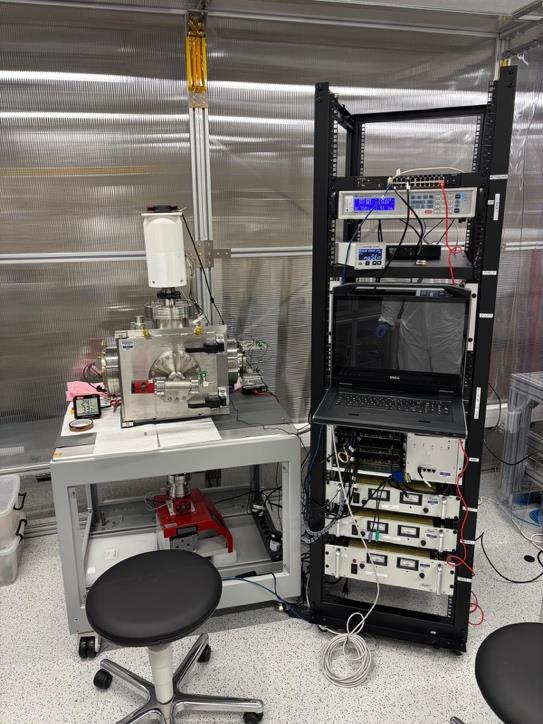
\includegraphics[width=0.7\linewidth]{figures/JHU_test_chamber_exterior.png}
    \caption[Test chamber JH2 at LSM]{Test chamber JH2 as commissioned at LSM, showing the stainless-steel vacuum cryostat with cryocooler (left) and the electronics rack housing the VME crate, ACMs, and DAQ server (right), located within the ISO-6 cleanroom.}
    \label{fig:JHUChamberExterior}
\end{figure}

\begin{itemize}

\item Cryostat and vacuum chain: The test system used a stainless-steel vacuum cryostat mounted on a wheeled cart for transport. A Pfeiffer HiCube 80 Eco turbomolecular pump sat below the chamber, electrically isolated from the test chamber via a ceramic vacuum fitting. The residual pressure inside the cryostat was monitored by a Pfeiffer PTR91 dual Pirani/cold cathode\footnote{Since the cold cathode operates via high-voltage glow discharge, which can generate detectable photons and electromagnetic interference, the gauge was powered off during CCD testing.} gauge and reached ${\lesssim}10^{-4}\text{\,mbar}$ at room temperature. The pump and pressure gauge had external Ethernet connections for monitoring (Pfeiffer CenterOne) and control (Perle Iolan DS1).
    
\item Thermal chain: The cryostat was equipped with a Cryotel GT cryocooler with active vibration cancellation. A 3D-printed shroud with a fan enclosed the air-side cooling fins to prevent overheating. Inside the cryostat, the aluminum CCD boxes were thermally coupled to the cryocooler cold end via a copper bar. A layer of Kapton tape electrically isolated the bar from the cryocooler, and a plastic KF fitting isolated the cryocooler body from the cryostat. Resistance temperature detectors (RTDs) were positioned on the cryocooler cold end, on the thermal bar, and on the outer CCD boxes (two RTDs). The RTDs and a resistive heater mounted to the copper bar were connected in a PID control loop with a Lakeshore 336 temperature controller via a custom vacuum-air interface board with D-sub connections. A PTFE table provided mechanical support to the CCD boxes, as well as thermal and electrical isolation from the chamber walls.

A key difference between the thermal chain used during surface testing and that used during underground testing was the active balancer controlling the cryocooler. Following surface testing, the cryocoolers were sent to Ametek for inspection and repair, as multiple issues were reported, including overcurrent incidents that caused instrument shutdown, audible ringing from the active balancer vibrating against the cryocooler, and low-frequency noise introduced by the active vibration control system. Despite Ametek technicians' intervention upon arrival and installation at LSM, the cryocooler configuration—consisting of an AVC balancer and a second-generation AVC controller—continued to exhibit overcurrent and low-frequency noise. 

A second-generation AVC balancer from Ametek resolved the overcurrent issue that prevented prolonged cryocooler operation. However, this AVC model consistently introduced low-frequency noise, resulting in overall readout noise levels higher than those previously observed. As a result, a first-generation AVC balancer was used throughout the testing, as it provided stable, continuous operation and acceptable noise levels. Figure~\ref{fig:psd_avc} shows the noise level evolution across three configurations:

\begin{itemize}
\item \textbf{Blue (July 3)}: Gen2 AVC, new controller from Ametek mid-June, Meanwell power supply
\item \textbf{Orange (July 10)}: Gen2 AVC, new controller from Ametek mid-June, Meanwell power supply
    \begin{itemize}
    \item Improved grounding configuration
    \end{itemize}
\item \textbf{Green (July 22, Current)}: Gen1 AVC, old controller sent from UW, Acopian power supply
\end{itemize}

\begin{figure}[H]
    \centering
    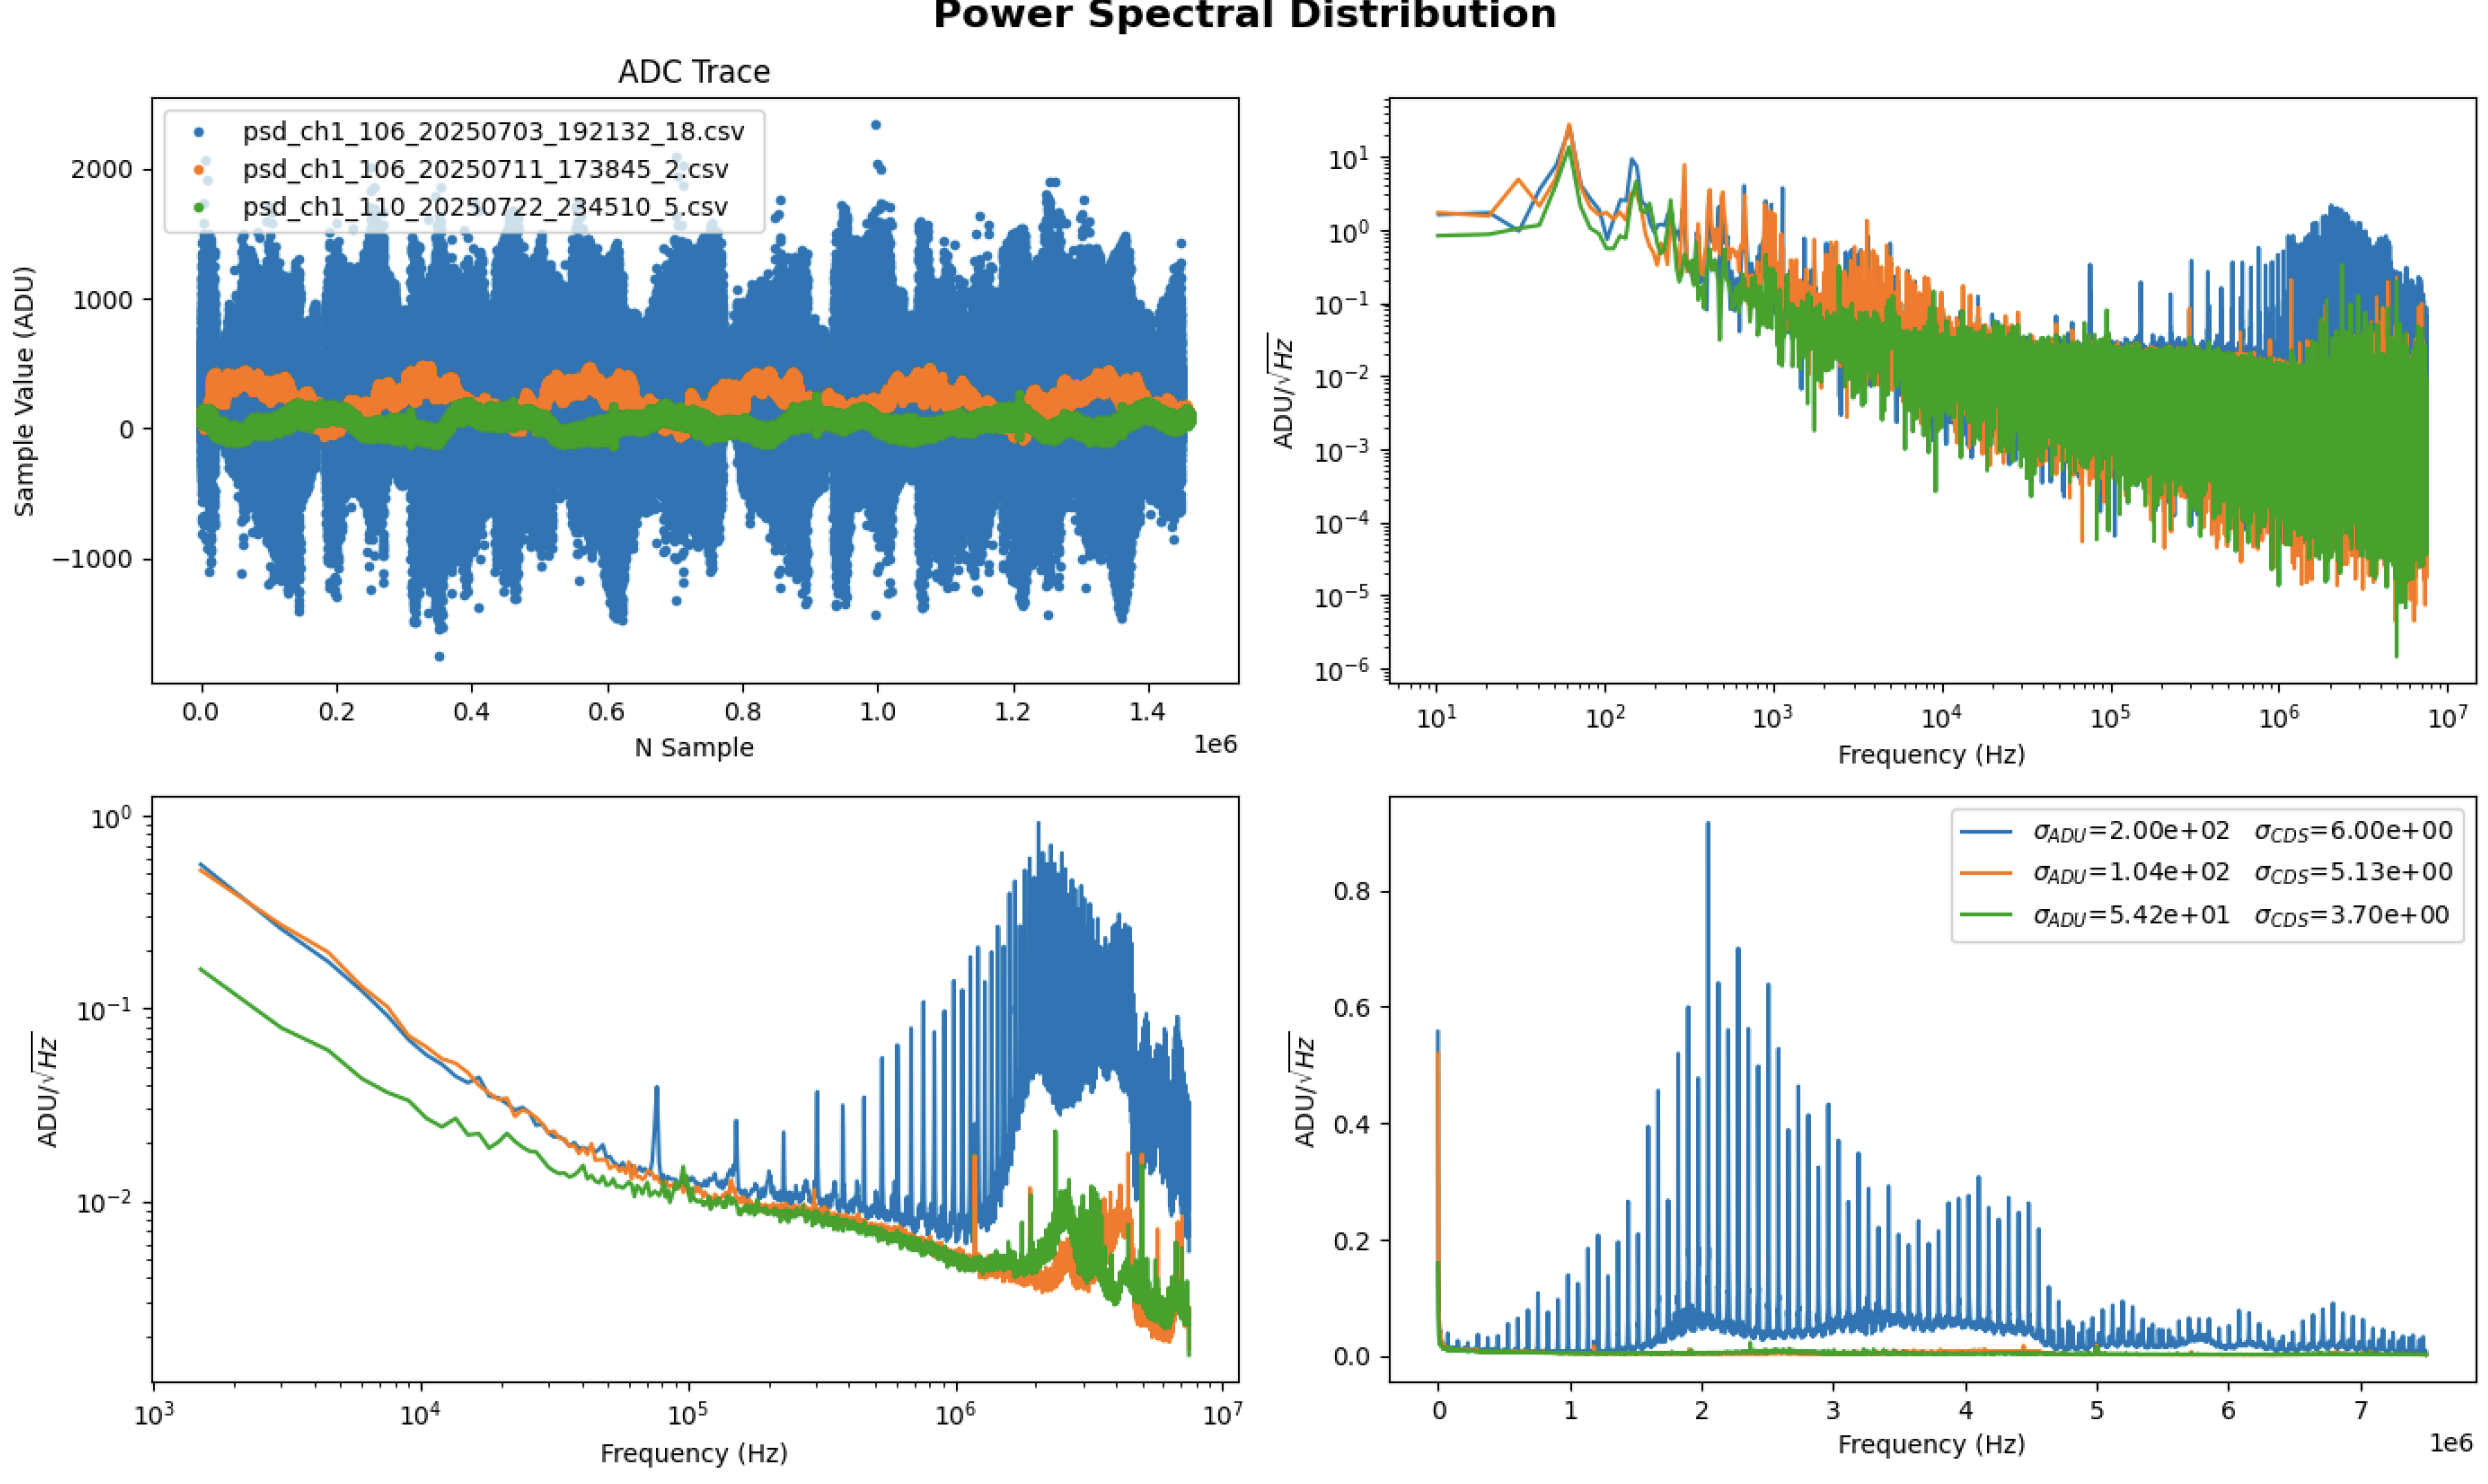
\includegraphics[width=0.95\linewidth]{figures/psd_avc_gen1_vs_gen2_plot.png}
    \caption[PSD comparison: AVC Gen.~1 vs.\ Gen.~2]{Power spectral distribution for the three configurations above. \emph{Top left}: raw ADC trace. \emph{Top right}: PSD vs.\ frequency (log-log). \emph{Bottom left}: PSD vs.\ frequency, zoomed. \emph{Bottom right}: PSD vs.\ frequency (linear), with fitted noise values $\sigma_{\mathrm{ADU}}=2.00\times10^{2}$, $\sigma_{\mathrm{CDS}}=6.00$ (blue); $\sigma_{\mathrm{ADU}}=1.04\times10^{2}$, $\sigma_{\mathrm{CDS}}=5.13$ (orange); $\sigma_{\mathrm{ADU}}=5.42\times10^{1}$, $\sigma_{\mathrm{CDS}}=3.70$ (green).}
    \label{fig:psd_avc}
\end{figure}
    
\item Detectors and electronics chain: Inside the cryostat, each CCD module flex cable plugged into a Kapton extension cable that carried the clocks, biases, and amplifier output signals. The extension cables were connected to a vacuum-air interface board with Samtec connections. Outside the chamber, three front-end boards (one per CCD die or module), plugged into the vacuum feedthrough, performed the initial signal amplification. High-speed twinax cables (Samtec ERCD-030-120.0-TBR-TTL-1-C) connected the front-end boards to the main electronics racks located outside the cleanroom.

\end{itemize}

In contrast to surface testing, all electronic components were placed on a rack within the cleanroom, adjacent to the testing setup. The main electronic components were grouped into two categories:

\begin{itemize}

\item Slow control: This system monitored and controlled the cryostat service equipment (cryocoolers, vacuum pumps, temperature controllers) using custom C-based back-end software with a PHP-based front-end interface \cite{DAMIC-M:2024ooa,slowcontrol}. The system communicated with the electronics modules over a local wired network, converting from serial protocols to TCP when necessary. The system logged status in a MySQL database, and triggered alarms if parameters exceeded predefined bounds. 

\item Data acquisition: This system handled CCD control and data taking. A Wiener VME195x crate housed the test chamber, which contained three Acquisition and Control Modules (ACMs), each connected to a front-end board on the cryostat. During module testing, the ACMs generated bias and clock voltages for the CCDs and processed their output signals through four channels, one per CCD \cite{Gaior:2023wfr}. A dedicated clock-synchronization board enabled synchronous ACM operation during CCD readout. A suite of Acopian linear power supplies provided low-noise DC voltages to the VME crates (±15 V, +30 V). An additional Linux server set the CCD operating parameters, executed readout, and served as local data storage.

\end{itemize}


\subsection{DAQ configuration}

Control and communication with each ACM board were performed using the local DAQ (LDAQ), comprising ACMDAQ, \texttt{acmpy}, a sequencer, and a decoder \todonote{we still need to add the citation for the ACMDAQ/acmpy GitHub repository and the SSM (Sravan?) thesis describing the LDAQ software stack.}. ACMDAQ is a C++ server that communicates directly with the ACM via hexadecimal messages over Ethernet. The Python package \texttt{acmpy} interfaces with ACMDAQ and provides high-level CCD control. The sequencer file, written in the LSST sequencer language \todonote{we still need to cite the LSST camera sequencer language reference, or the DAMIC-M internal note describing its adaptation.}, is compiled within \texttt{acmpy} and transmitted to the ACM FPGA to define the clock sequencing. Each ACM board is operated by an independent LDAQ instance, which can run either standalone or under the central DAQ (CDAQ) \todonote{we still need to cite the CDAQ software/documentation.}.

For each tested module, a dedicated sequencer and configuration file were prepared to define timing and voltage parameters. Table~\ref{tab:sequencer_timing_dm13} summarizes the timing parameters used for production modules. The table shows an example corresponding to a full-array image acquired with no binning, no image cuts, and single-skip (NDCM=1) readout.
%
\begin{table}[H]
\centering
\caption{Key geometry and timing parameters defined in the LDAQ sequencer used for module testing. Unless noted otherwise, delays are specified in FPGA clock cycles.}
\label{tab:sequencer_timing_dm13}
\begin{tabular}{@{}ll@{}}
\toprule
\textbf{Category} & \textbf{Parameter (value)} \\
\midrule
Image format & NROW = 1400 (binned rows), NCOL = 6300 (binned columns) \\
Binning & NPBIN = 1 (parallel), NSBIN = 1 (serial) \\
Skipper sampling & NDCM = 1, NDCMPRE = 0 \\
Cuts & NROWPRE = 0, NROWPOST = 0, NCOLPRE = 0, NCOLPOST = 0 \\
Exposure & EXPOSURE = 500 \\
PSD timing & NPSD = 100, delayPSD = 10000, delayDef = 100 \\
Serial-register wait & NVWAIT = 0 \\
Vertical transfer & delay\_Va = 6000, delay\_Vb = 6000 \\
Horizontal transfer & delay\_Ha = 1800, delay\_Hb = 1800, delay\_Hc = 1800 \\
CDS/DSI integration & delayInt = 1000 \\
Reset gate & delayRGL = 27, delayRGH = 800 \\
Summing well & delaySWH = 30, delaySWL = 350 \\
Output gate & delayOGL = 48, delayOGH = 3 \\
Dump gate & delayDGL = 27, delayDGH = 47 \\
FPGA clock & clockperiod = 10 ns \\
\bottomrule
\end{tabular}
\end{table}
%
In addition to the sequencer file, a configuration file in \texttt{.bcf} format specifies the bias and clock-rail voltages applied during operation. The configuration parameters corresponding to the example above are summarized in Table~\ref{tab:config_dm13}.

\begin{table}[H]
\centering
\caption{Configuration file parameters for module testing. Voltages are given in volts.}
\label{tab:config_dm13}
\begin{tabular}{@{}ll@{}}
\toprule
\textbf{Category} & \textbf{Parameter (value)} \\
\midrule

\multicolumn{2}{l}{\textit{Sequencer mapping}} \\
Vertical transfer & Vtransfer21 \\
Horizontal transfer & HtransferUU \\
Channel mapping & ch0=D,\; ch1=C,\; ch2=A,\; ch3=B \\[4pt]

\multicolumn{2}{l}{\textit{Bias voltages (V)}} \\
VDD1, VDD2 & -19 \\
VR1, VR2 & -3 \\
VDRAIN1, VDRAIN2 & -23 \\
VSUB & 45 \\[4pt]

\multicolumn{2}{l}{\textit{Clock offsets (V)}} \\
OFS\_RS1, OFS\_RS2, OFS\_CLK & -10 \\[4pt]

\multicolumn{2}{l}{\textit{Parallel clock rails (V)}} \\
V1\_A (H/L) & 9.9 / 7.9 \\
V1\_B (H/L) & 9.9 / 7.7 \\
V2\_C (H/L) & 9.9 / 7.9 \\
V3\_A (H/L) & 9.9 / 7.9 \\
V3\_B (H/L) & 9.9 / 7.7 \\[4pt]

\multicolumn{2}{l}{\textit{Transfer gate rails (V)}} \\
TG\_A (H/L), TG\_B (H/L) & 7.4 / 7.4 \\[4pt]

\multicolumn{2}{l}{\textit{Serial clock rails (V)}} \\
H1\_A (H/L) & 9.5 / 6.7 \\
H1\_B (H/L) & 9.5 / 6.5 \\
H2\_C (H/L) & 9.0 / 6.7 \\
H3\_A (H/L) & 9.5 / 6.7 \\
H3\_B (H/L) & 9.5 / 6.5 \\[4pt]

\multicolumn{2}{l}{\textit{Output stage rails (V)}} \\
SW\_1 (H/L), SW\_2 (H/L) & 1.0 / -6.0 \\
OG\_1 (H/L), OG\_2 (H/L) & 0.0 / -6.0 \\
RG\_1 (H/L), RG\_2 (H/L) & 9.0 / 3.0 \\
DG\_1 (H/L), DG\_2 (H/L) & 0.0 / -5.0 \\

\bottomrule
\end{tabular}
\end{table}

The amplifier wire-bonding configuration and corresponding ACM channel mapping are shown in Table~\ref{tab:amp_mapping}. The charge-transfer direction, defined through sequencer and configuration function pointers, depends on the bonding configuration to ensure charge transfers toward the active output amplifiers. For the configuration shown here, the vertical transfer pointer was set to \texttt{Vtransfer21}.

\begin{table}[H]
\centering
\caption{Amplifier wire-bonding configuration and channel mapping for the CCDs within the module.}
\label{tab:amp_mapping}
\begin{tabular}{@{}lcccc@{}}
\toprule
 & \textbf{CCD A} & \textbf{CCD B} & \textbf{CCD C} & \textbf{CCD D} \\
\midrule
Bonded amplifiers & U2, L2 & U2, L2 & U1, L1 & U1, L1 \\
ACM channels      & 2, 3   & 3, 2   & 0, 1   & 1, 0   \\
\bottomrule
\end{tabular}
\end{table}


\subsection{Image list}
A total of seven image types were acquired at high (185 K) and low (135 K) temperatures to characterize detector performance under different operating conditions. The datasets include full-array exposures, serial-register readouts, and multi-skip images. Table~\ref{tab:image_summary} summarizes the image configurations and their primary objectives.


\begin{table}[H]
\centering
\caption{Summary of images acquired during module testing. Exposure times are given in seconds. Dimensions correspond to the binned image size.}
\label{tab:image_summary}
\begin{tabular}{@{}lllllll@{}}
\toprule
\textbf{Image} &
\begin{tabular}{@{}c@{}}\textbf{Temp}\\ \small(K)\end{tabular} &
\begin{tabular}{@{}c@{}}\textbf{Exposure}\\ \small(s)\end{tabular} &
\begin{tabular}{@{}c@{}}\textbf{Dimensions}\\ \small(rows × cols)\end{tabular} &
\begin{tabular}{@{}c@{}}\textbf{Binning}\\ \small(P,S)\end{tabular} &
\textbf{NDCM} &
\textbf{Mode} \\
\midrule

Image\_1 & 185 & 3   & 80×340   & 20×20 & 1   & Active \\

Image\_2 & 185 & 3   & 20×6400  & 1×1   & 1   & Serial register \\

Image\_3\_185 & 185 & 3   & 30×640   & 1×1   & 500 & Serial register \\

Image\_4\_185 & 185 & 500 & 1600×6300 & 1×1   & 1   & Active \\

\midrule

Image\_3\_135 & 135 & 3   & 30×640   & 1×10  & 500 & Serial register \\

Image\_4\_135 & 135 & 500 & 1600×6300 & 1×1   & 1   & Active \\

Image\_5 & 135 & 500 & 480×1280  & 1×1   & 500 & Cropped region \\

Image\_6 & 135 & 500 & 160×640   & 10×1  & 500 & Cropped region \\

Image\_7 & 135 & 500 & 1600×64   & 1×10  & 500 & Cropped region \\

\bottomrule
\end{tabular}
\end{table}

At high temperature (185 K), Image\_1 was used as an installation and basic functionality check with coarse binning to allow rapid verification of detector operation after installation. Image\_2 provided a serial-register readout to identify serial-register defects. Image\_3\_185 was acquired in serial-register mode with 500 skips to evaluate skipper readout performance. Image\_4\_185 consisted of a full-array exposure used to identify column defects and to evaluate readout noise.

At low temperature (135 K), Image\_3\_135 was acquired in serial-register mode with multi-skip readout to evaluate Skipper performance under nominal operating conditions. Image\_4\_135 was a full-array long exposure used to study CTI, readout noise, and amplifier glow, as well as to visualize prominent column defects. In addition, this image was used to evaluate keV-scale energy reconstruction by examining Fe-55 events deposited across the full array. Images\_5–7 were acquired to study a region of the CCD array with a high density of Fe-55 events in both the surface and the bulk. These images were taken in multi-skip readout mode with different binning configurations. CTI studies were also performed using these datasets.

\newpage

% =====================================================
%            Procedure for data acquisition
% =====================================================
\section{Procedure for data acquisition}
\label{sec:procedure}

Each module installation was coordinated between on-site installers and off-site testers, with three modules installed per batch. Before installation, on-site testers verified that the previous testing cycle had concluded, that the chamber was at room temperature and atmospheric pressure, and that the modules could be safely removed and stored in the nitrogen cabinet. The team then retrieved the next batch of three production modules from the nitrogen cabinet for installation.

Figure~\ref{fig:MODULE_INSTALLATION} shows an example of a module batch installed inside the test chamber, with the production module having the highest ID positioned to the left of the cold finger and the remaining two in descending order to the right. The modules' flex cables were connected to extensions F, D, and E, corresponding to ACM boards 106, 109, and 110, respectively.

\begin{figure}[H]
    \centering
    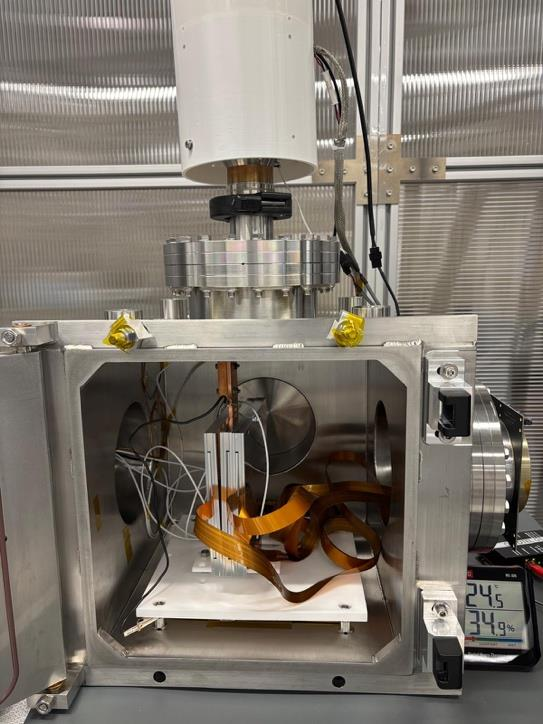
\includegraphics[width=0.6\linewidth]{figures/module_batch_installed.png}
    \caption[Module batch installed in the test chamber]{A batch of three production modules (DM03, DM02, DM01, left to right) installed inside test chamber JH2, with flex cables routed to the vacuum-air interface board. Following the convention described in the text, DM03 (highest ID) is positioned to the left of the cold finger, with DM02 and DM01 in descending order to the right.}
    \label{fig:MODULE_INSTALLATION}
\end{figure}

After installation, the chamber was closed and pumped down to ${\leq}1\times 10^{-4}\,\mathrm{mbar}$ at room temperature to remove residual volatile compounds and prevent condensation on cold surfaces. Cooldown then proceeded at a controlled rate of ${<}0.5\,\mathrm{K/min}$ to avoid thermal stress on the silicon. Approximately five hours were required to reach the first target temperature of 185 K. Thermal stability was defined by a temperature variation of the CCD boxes\footnote{Dedicated studies show that the temperature of the silicon die is within ${\sim}$5 K of the box temperature and that the temperature gradient across the silicon is negligible.} of less than $0.01\,\mathrm{K}$ over a five-minute interval.

Once stable at 185 K, an installation check was performed. The CCDs were powered on with $V_{\mathrm{DD}}$ set to $-10$ V, allowing only the highest-energy tracks to be visible. Image\_1 (Table~\ref{tab:image_summary}) was acquired to verify proper installation of all modules and to obtain a rapid measurement of the readout noise. After confirming nominal operation, cooldown continued to 135 K and required approximately two additional hours.

During cooldown, erase–epurge sequences were executed to reduce dark-current levels associated with surface traps formed during power-up. At 185 K, the following sequence was performed:

\begin{itemize}
    \item Erase $\rightarrow$ Flush $\rightarrow$ Epurge $\rightarrow$ Flush $\rightarrow$ Erase $\rightarrow$ Flush $\rightarrow$ Epurge $\rightarrow$ Flush
\end{itemize}

After completing the 185 K sequence, the chamber continued cooling at ${<}0.5\,\mathrm{K/min}$ while the CCDs were kept in continuous flush mode. Once thermal stability was achieved at 135 K, a second sequence was performed:

\begin{itemize}
    \item Erase $\rightarrow$ Flush $\rightarrow$ Erase $\rightarrow$ Flush
\end{itemize}

During both procedures, $V_{\mathrm{DD}}$ was turned off (set to $-6$ V) and restored only immediately before image acquisition at 135 K.

In contrast to on-surface testing, the high-temperature measurements in this campaign were performed after low-temperature operation, during the controlled warm-up from 135 K toward room temperature. This sequence mimics the thermal cycle implemented in the LBC, in which erase and epurge steps are performed at 185 K and 135 K (with only epurge at 135 K). Unlike standard LBC operations, these tests performed no erase or epurge steps at 150 K.


\subsection{Acquisition sequence} 

The following image acquisition sequence was performed at 135 K and 185 K. The table below summarizes the number of exposures for each image type and the corresponding readout times.

\paragraph{Acquisition at 135 K}

\begin{itemize}
    \item 6 $\times$ Image\_4\_135 \hfill (readout time per image: 47\,min 34\,s)
    \item 3 $\times$ Image\_5 \hfill (readout time per image: 2\,hr 58\,min 28\,s)
    \item 4 $\times$ Image\_6 \hfill (readout time per image: 31\,min 33\,s)
    \item 2 $\times$ Image\_7 \hfill (readout time per image: 1\,hr 3\,min 52\,s)
    \item 6 $\times$ Image\_3\_135 \hfill (readout time per image: 6\,min 0\,s)
\end{itemize}

The total acquisition time at 135 K was 18\,hr 30\,min 44\,s.

After completion of the 135 K dataset, the system was warmed back to 185 K under controlled conditions. Once thermal stability at 185 K was re-established, the following set of images was acquired.

\paragraph{Acquisition at 185 K}

\begin{itemize}
    \item 6 $\times$ Image\_4\_185 \hfill (readout time per image: 47\,min 34\,s)
    \item 6 $\times$ Image\_3\_185 \hfill (readout time per image: 5\,min 38\,s)
    \item 1 $\times$ Image\_2 \hfill (readout time: 44\,s)
    \item 1 $\times$ Image\_1 \hfill (readout time: 2\,min 12\,s)
\end{itemize}

The total acquisition time at 185 K was 5\,hr 22\,min 8\,s. This data-acquisition sequence allowed two module batches to be tested each week.

% \subsection{Online quality checks}
% Baseline stability, out-of-range pixels, saturation, readout artifacts, unexpected pattern noise, etc.

% =====================================================
%          High-temperature image analyses
% =====================================================
\newpage
\section{High-temperature image analyses}
\label{sec:hightemp}

As in the die- and module-level surface testing, a series of measurements at 185~K were performed to efficiently identify defects in each CCD within each module. Although 185~K is not the nominal operating temperature of the DAMIC-M experiment, additional images were acquired at this temperature to further characterize each module's overall Skipper-CCD performance. These measurements were used to evaluate key performance metrics, including readout noise, single-electron resolution, dark current, and gain, and to investigate potential temperature-dependent effects.


% \subsection{Skipper performance}

\subsection{Column defects in CCD active region}
\label{sec:column_defects}
To identify defects and glowing, six Image\_4 were collected at 185 K. Baseline subtraction was performed on a row-by-row basis using the median of the $x$-overscan region. A composite image was then constructed by taking the median value of each pixel across the image stack. This procedure suppresses particle tracks and pixel-level noise, thereby enhancing the visibility of defects and glowing features that persist across all images.

Column defects were identified by analyzing the median signal value of each column in the composite image. For a given column index $j$, the column median $C_j$ was computed as
\begin{equation}
C_j = \mathrm{median}_{i}\left( I_{ij} \right),
\end{equation}
where $I_{ij}$ denotes the pixel value at row $i$ and column $j$.
To identify anomalous columns, $C_j$ was compared to a local running median $\tilde{C}_j$ computed over a sliding window of 40 columns centered on column $j$,
\begin{equation}
\tilde{C}_j = \mathrm{median}\left( C_{j-w}, \ldots, C_{j+w} \right),
\end{equation}
with $w=20$. The local dispersion was quantified using the median absolute deviation (MAD),
\begin{equation}
\mathrm{MAD}_j = \mathrm{median}\left( \left| C_k - \tilde{C}_j \right| \right), \quad k \in [j-w, j+w].
\end{equation}

Columns were flagged as defective if their median value deviated significantly from the local running median,
\begin{equation}
C_j - \tilde{C}_j > 6 \times \mathrm{MAD}_j \quad \text{(hot column)},
\end{equation}
\begin{equation}
C_j - \tilde{C}_j < -6 \times \mathrm{MAD}_j \quad \text{(cold column)}.
\end{equation}

This procedure produces a defect map detailing the locations, types, and numbers of flagged columns for each CCD in each module. Figure~\ref{fig:composite_image} shows composite-image defect maps for the four CCDs in module DM06. In addition, the pixel-array values in the composite image are significantly higher than those in the overscan regions due to charge accumulated from dark current, giving rise to the steps visible in Fig.~\ref{fig:composite_image}. For this same type of image collected at low temperature, these overscan steps are used in one of the charge-transfer inefficiency (CTI) studies described in Section~\ref{sec:CTI}.

%
\begin{figure}[H]
    \centering
    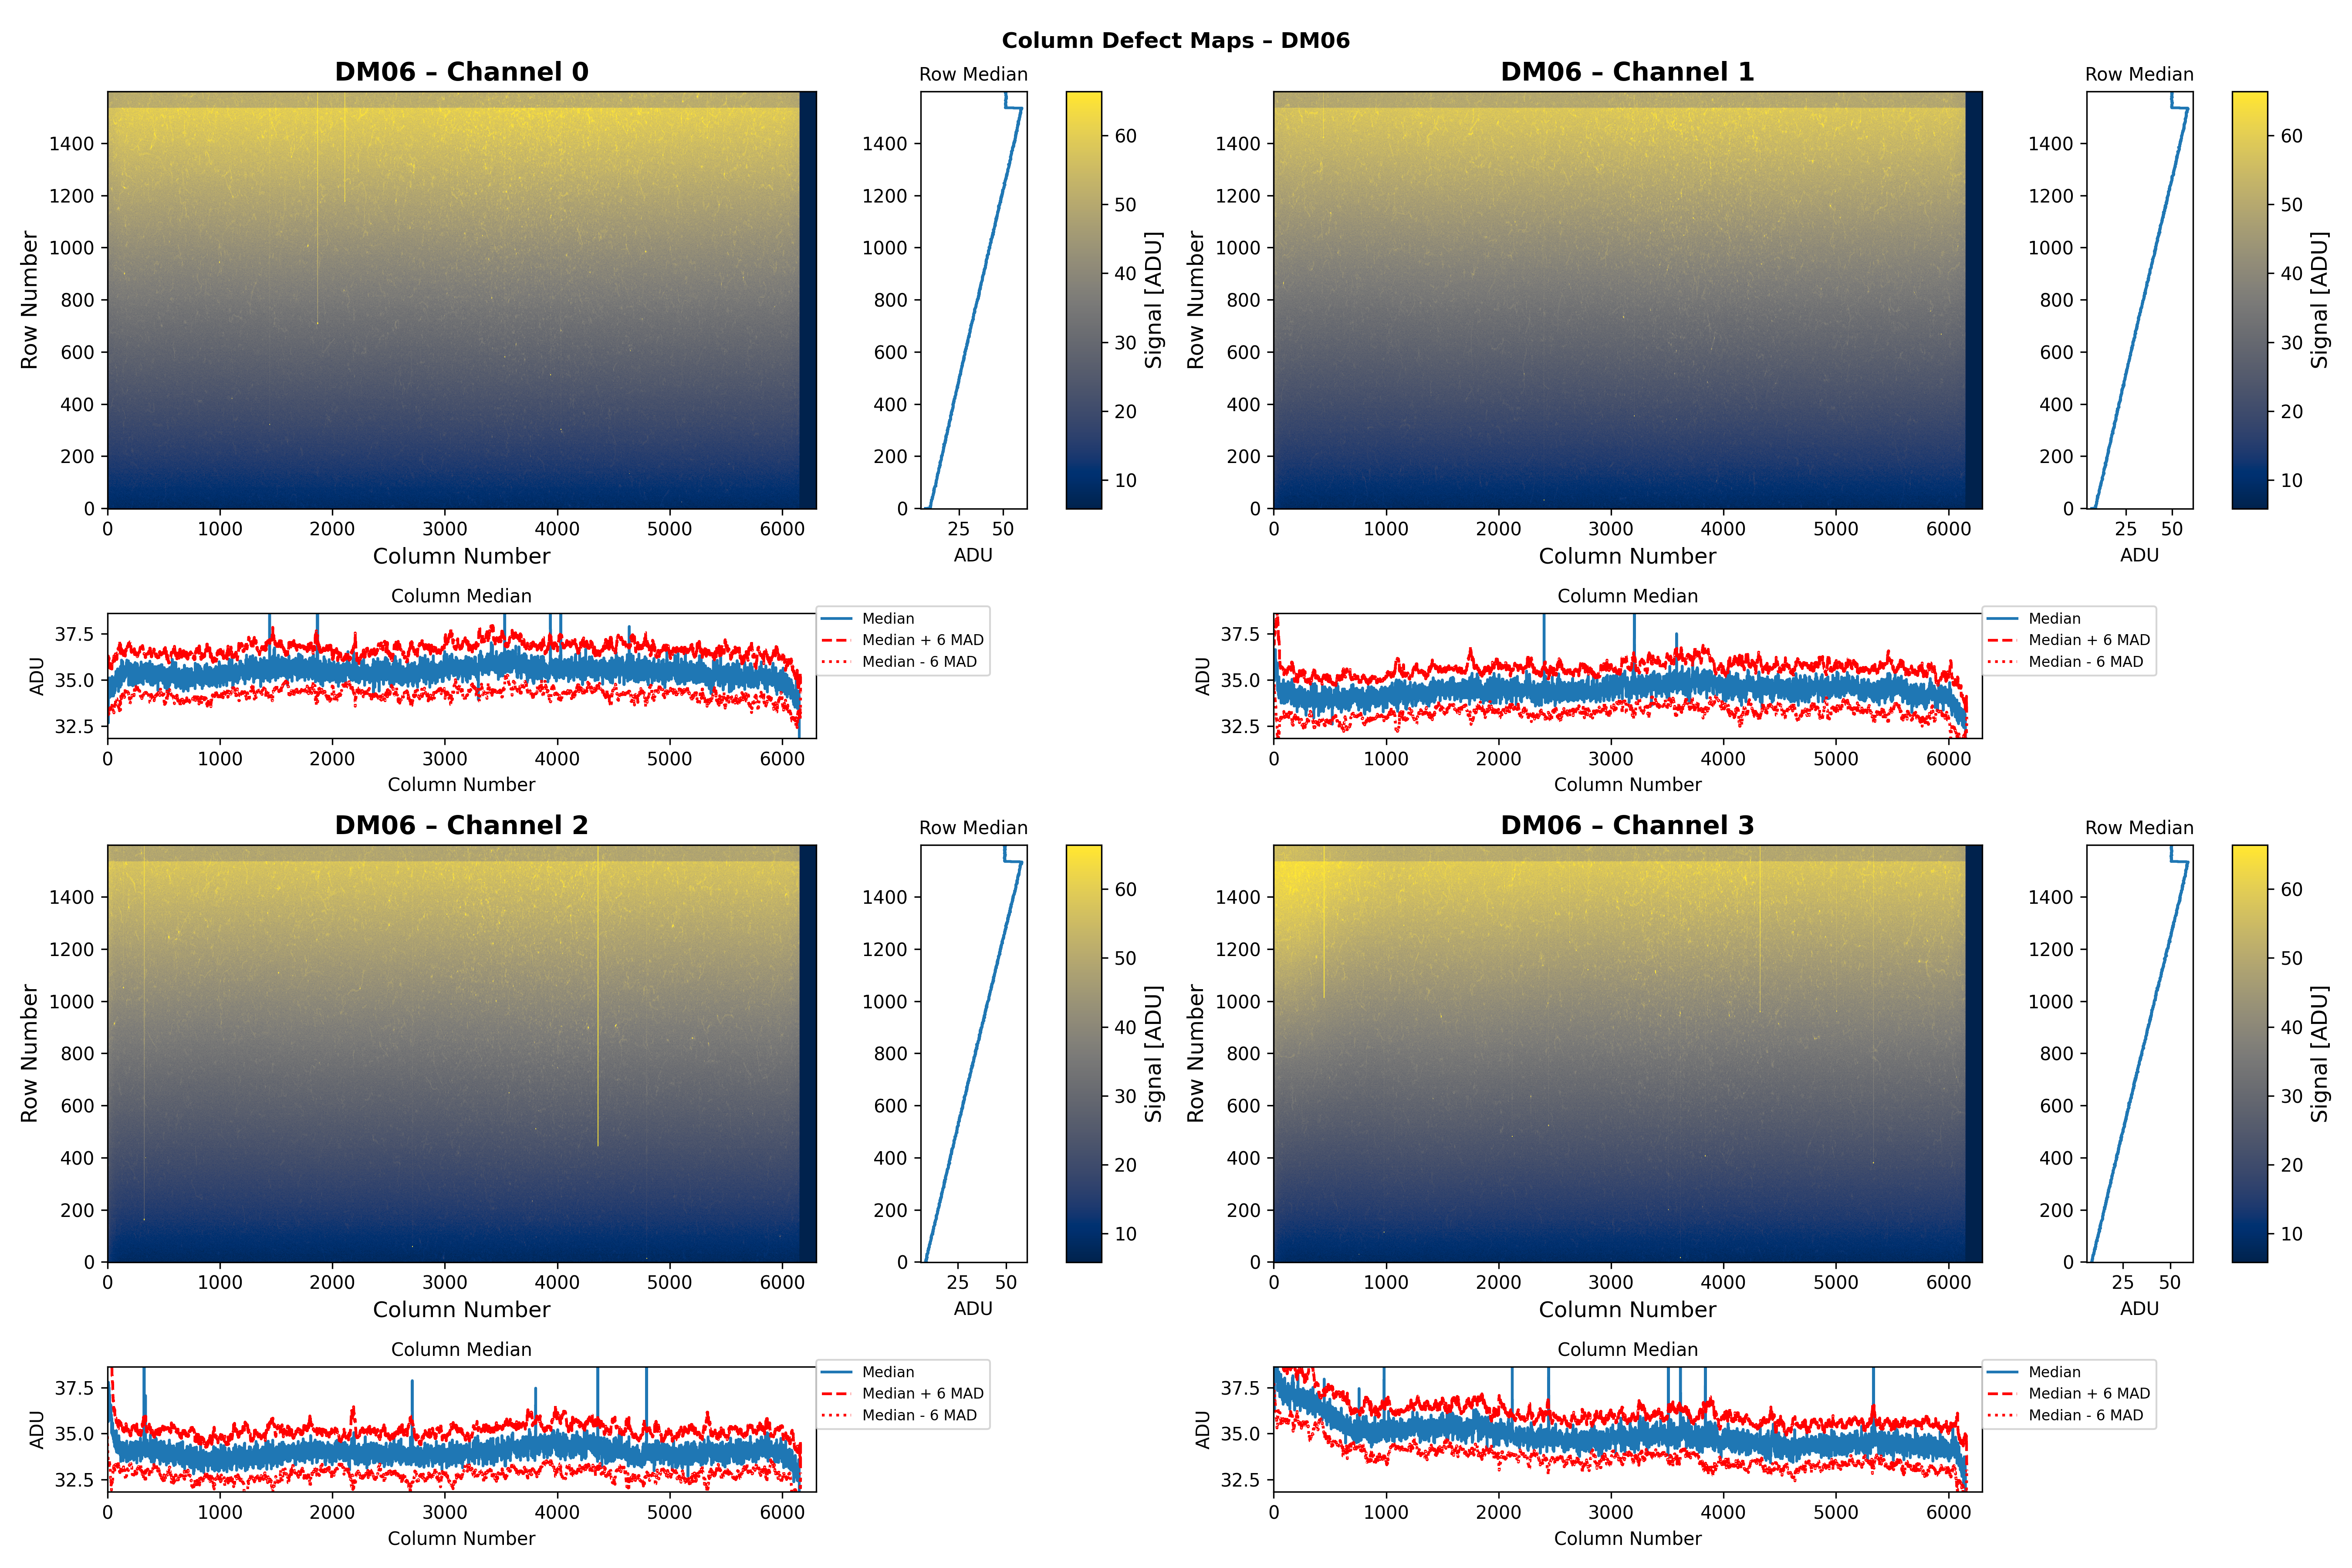
\includegraphics[width=1\linewidth]{figures/DM06_col_defect_map.png}
    \caption[Composite image analysis]{Column defect map obtained from a composite image built from six images for each CCD in module DM06. Particle tracks are filtered out, revealing hot columns (bottom panel). The $x$- and $y$-overscan steps are visible in each panel.
    }
    \label{fig:composite_image}
\end{figure}
%

Figure~\ref{fig:column_defects} summarizes the number of column defects identified in each CCD for all production modules using the 185~K composite Image\_4 dataset. For each module, defects were counted independently for each CCD, following the procedure described above. 

The gray band represents the mean defect count across all CCDs and modules, with a width corresponding to $\pm 1\sigma$ of the distribution. The dashed horizontal line indicates the global mean value of 9.91 hot columns per CCD. 
A subset of modules exhibits noticeably higher column-defect counts relative to the overall distribution. In particular, modules DM-08, DM-16, DM-17, DM-22, DM-23, DM-26, and DM-27 show elevated defect counts in at least one CCD, with some extensions exceeding 20 defective columns. Among these, DM-08 and DM-17 present the most pronounced outliers, with individual CCDs approaching or exceeding 25 defective columns. DM-23 and DM-26 also display consistently high counts across multiple CCDs within the same module. These modules contribute significantly to the upper tail of the defect-count distribution and therefore warrant closer inspection in subsequent analyses.

Module DM-08 contains a large column defect in CCD A that produces amplifier glow and elevated dark-current levels in the other extensions. As a result, this module will not be included in the final detector array.


\begin{figure}[H]
    \centering
    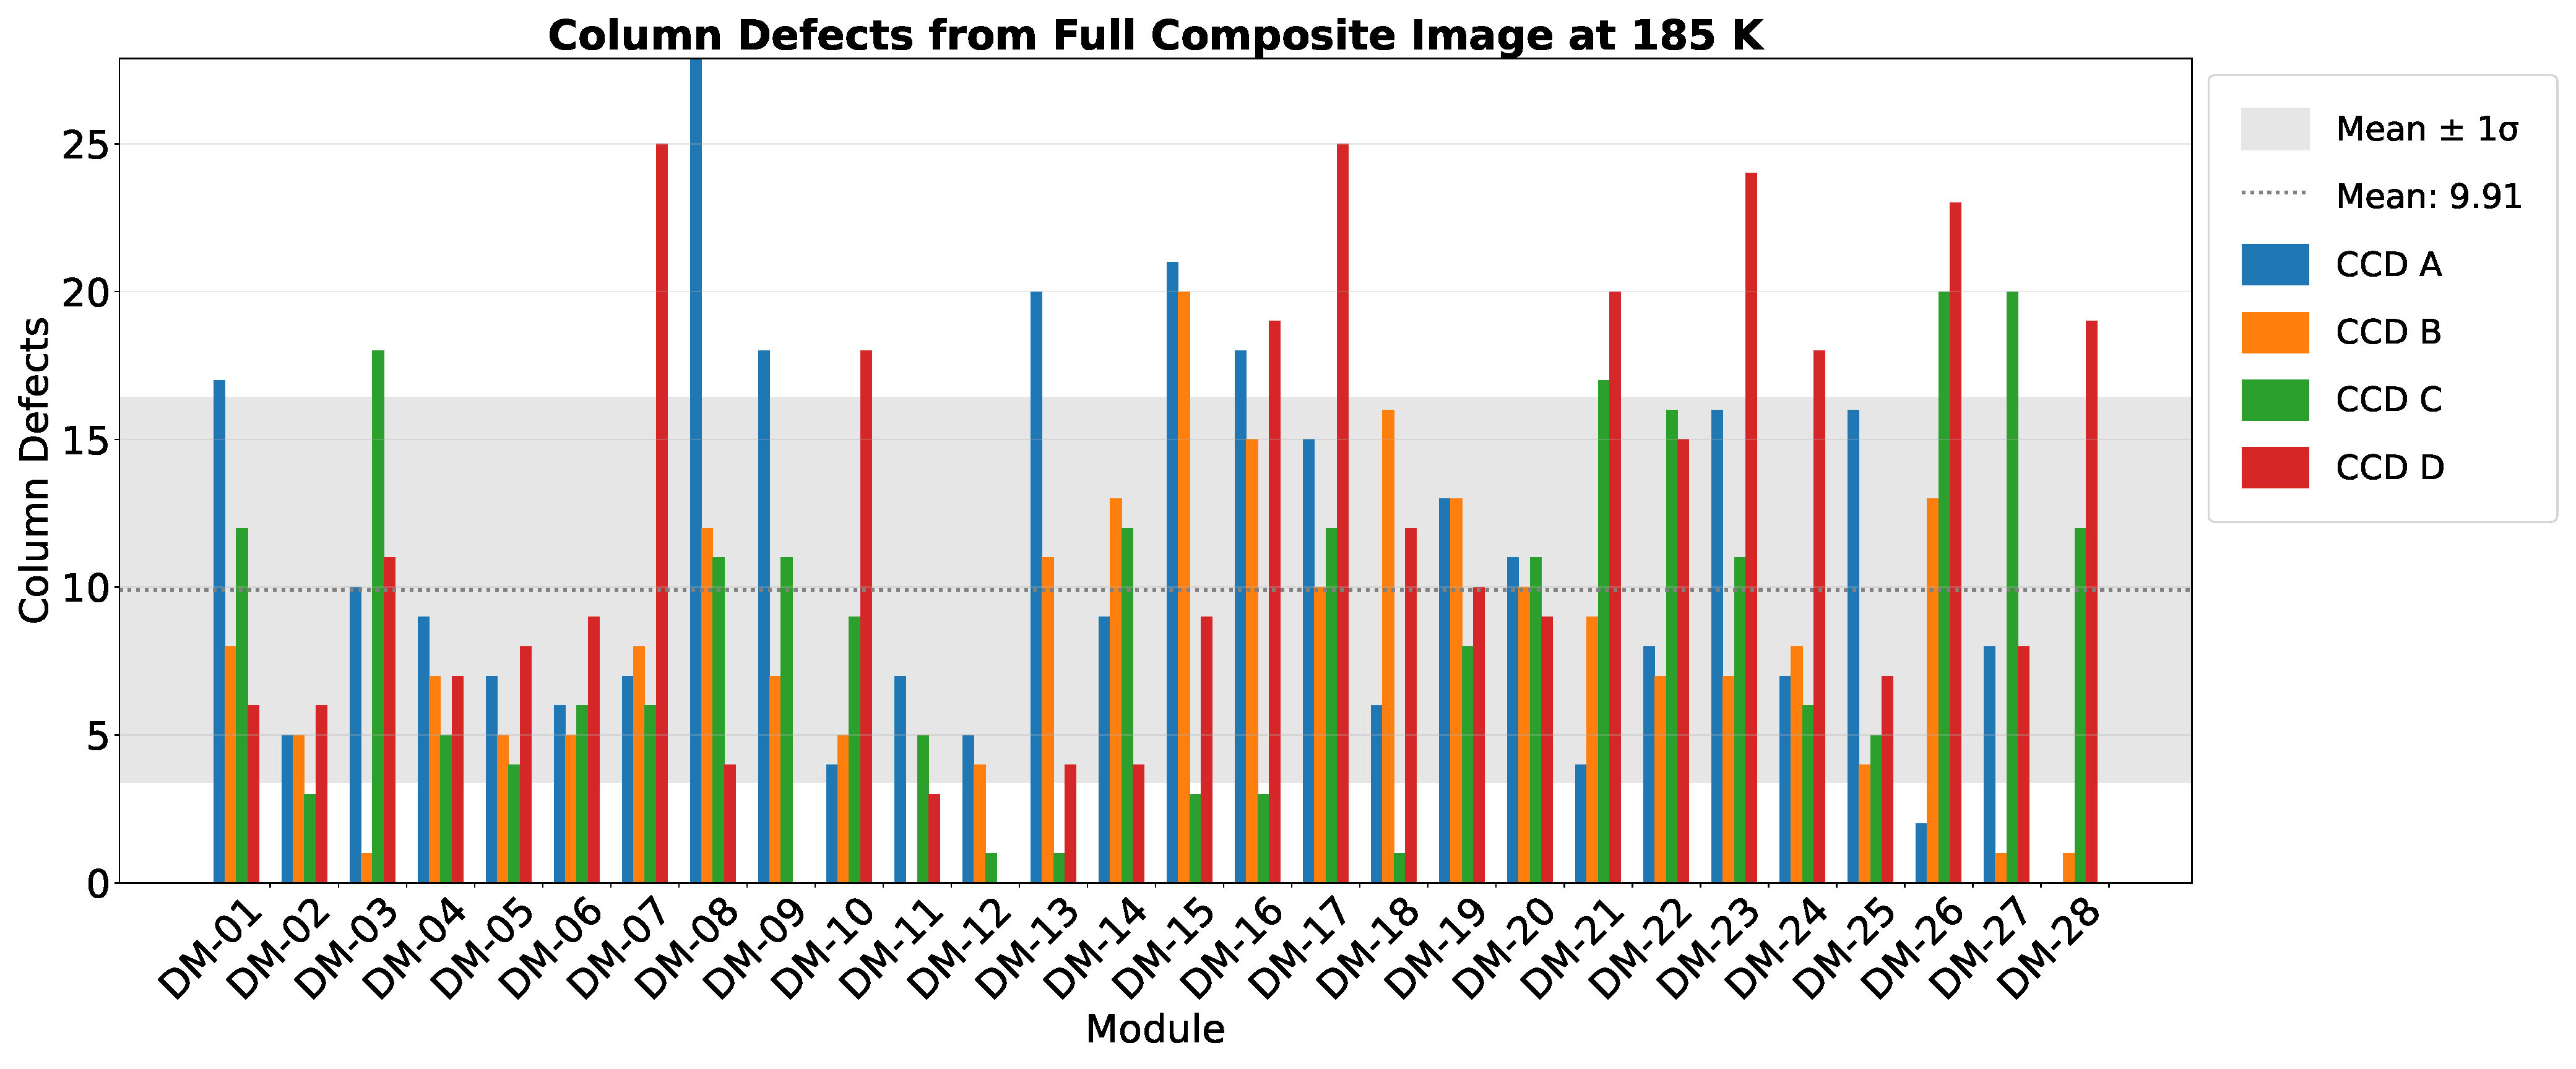
\includegraphics[width=1\linewidth]{figures/image4_high_column_defects_all_modules.pdf}
    \caption[Composite image analysis]{Number of column defects identified from the composite Image\_4 dataset at 185~K for each CCD (A–D) across all production modules. The gray band indicates the mean defect count $\pm 1\sigma$ across the full dataset, and the dashed horizontal line marks the global mean value of 9.91 defects per CCD.
    }
    \label{fig:column_defects}
\end{figure}



\subsection{Serial register defects}

In a serial register (SR) image, charge from the pixel array is not transferred into the serial register. Instead, the SR itself is exposed for 2~s to allow charge to accumulate before being clocked and read out. This procedure is repeated 20 times, producing an image in which each row corresponds to a successive readout of the serial register.

Unlike full-array images, serial-register images do not contain two-dimensional particle tracks. Charge deposition in the serial register appears as horizontal streaks across the image, as illustrated in Fig.~\ref{fig:DM18_SR_defects} for the four CCDs in module DM-18. A serial-register defect appears as a vertical column of excess charge that persists across multiple readouts.
%
Defects in both serial registers of each CCD were identified using the same median absolute deviation MAD-based algorithm described in Section~\ref{sec:column_defects}, applied to the column-wise median signal.


\begin{figure}[H]
    \centering
    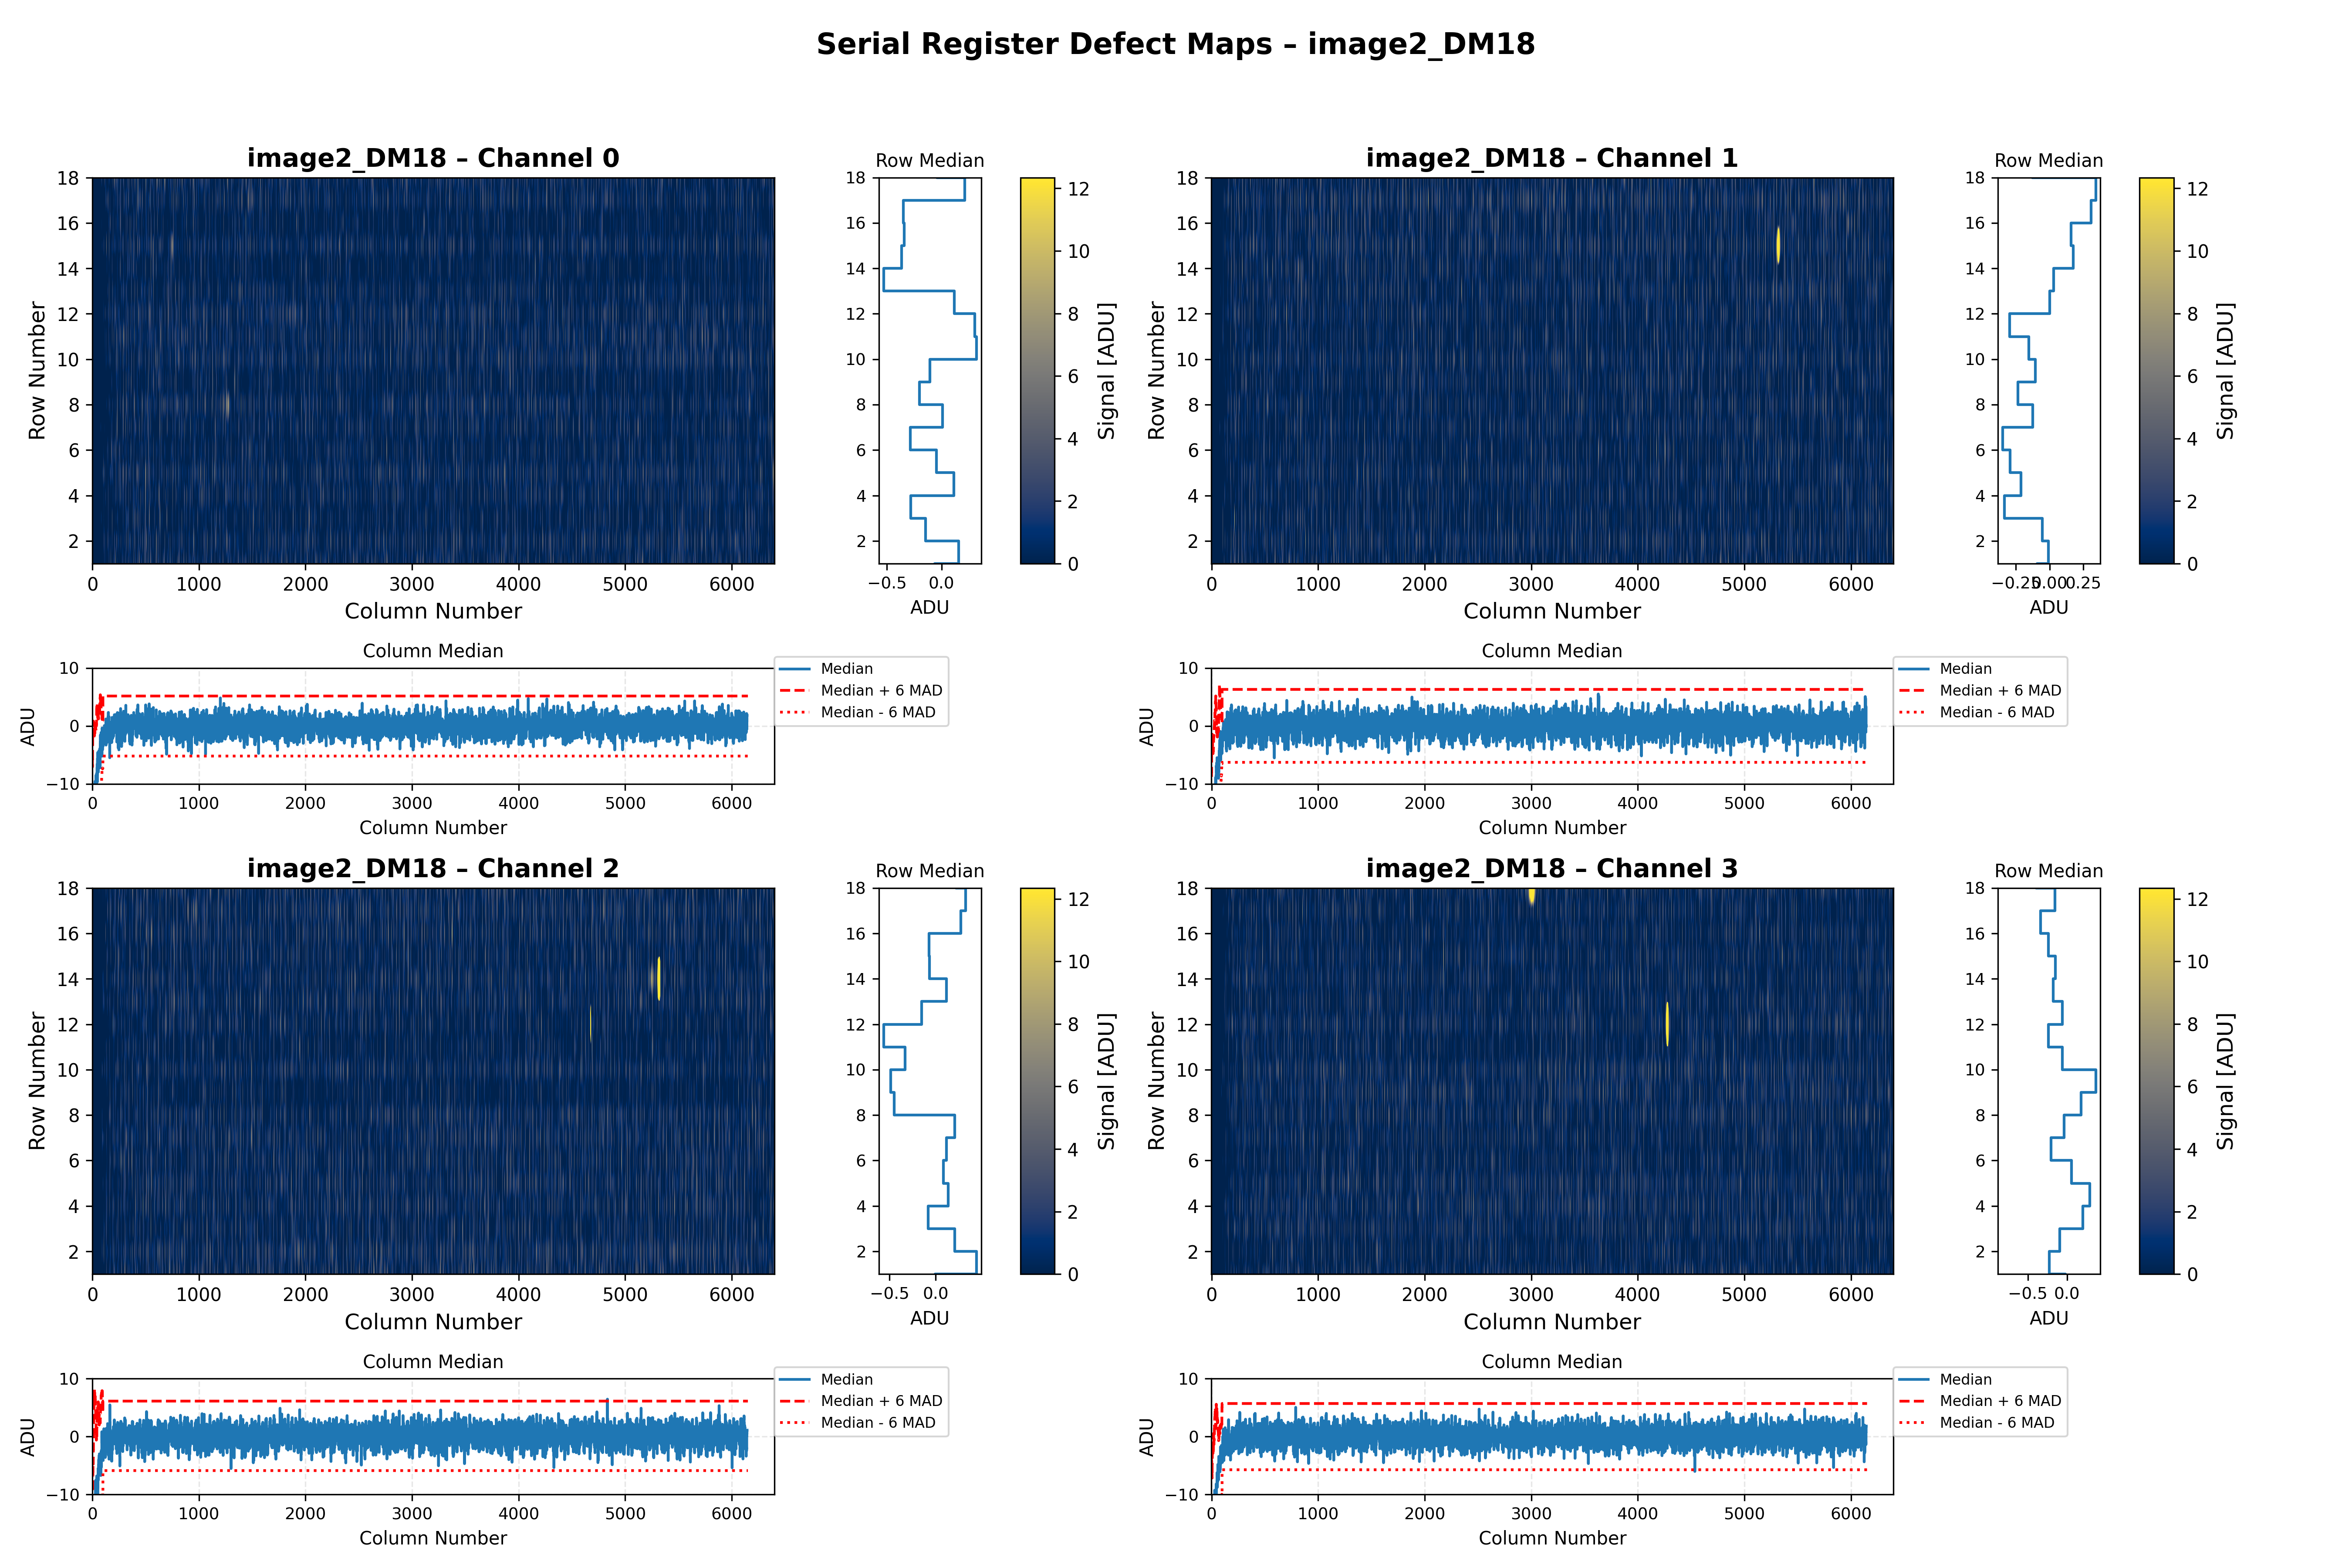
\includegraphics[width=1\linewidth]{figures/image2_high_file_DM18.png}
    \caption[Composite image analysis]{Number of SR defects identified from the composite Image\_2 dataset at 185~K for each CCD (A–D) in module DM18.
    }
    \label{fig:DM18_SR_defects}
\end{figure}

Across all modules and CCDs, the serial-register defect count remains low, with a global mean of 0.24 defects per CCD. Most CCDs show no detectable defects, while a small subset shows a single defective column in the serial register. No CCD was observed to contain more than one serial-register defect. 
%
A limited number of modules contain serial-register defects in more than one CCD extension. In particular, modules DM-05, DM-06, DM-13, DM-18, DM-20, and DM-23 each show defects in at least two CCDs. Nevertheless, even in these cases, the defect multiplicity per CCD remains limited to a single column, and the overall incidence of defects remains low across the production set.



\FloatBarrier

% =====================================================
%           Low-temperature image analyses
% =====================================================
\newpage
\section{Low-temperature image analysis}
\label{sec:lowtemp}
\subsection{Skipper performance}
DAMIC-M CCDs are operated in skipper mode to achieve single-electron resolution. Nominal skipper performance was verified by reading out 630 $x$-overscan pixels with 500 NDCMs.
At 135\,K, the test system's dark current is greatly reduced relative to higher-temperature operation. To estimate skipper performance under these conditions, 10 pixels from the serial register were transferred into the floating gate before measurement to ensure sufficient charge in the image pixels. This was done by collecting six \texttt{Image\_3\_135}.

The distribution of pixel values, averaged over the NDCMs, was fit with a Poisson distribution convolved with a Gaussian. The distance between consecutive peaks provides an estimate of the amplifier gain (in ADU/$e^-$), while the width of the peaks (measured as the standard deviation) provides an estimate of the readout noise.
The Poisson rate parameter $\lambda$ provides the average charge collected per pixel, which is proportional to the serial register dark current plus clock-induced charge (CIC). CIC arises from the rapidly changing electric fields caused by voltage swings of the gates during charge transfer and depends on the clock amplitude and rise time~\cite{Oscura:2023qik}. Serial clocks are the primary contributors to CIC, since they swing at a higher frequency than parallel clocks.

Figure~\ref{fig:DM09_SE_fits} illustrates the Poisson-convolved-Gaussian fits to the pixel charge distributions in all CCDs of module DM-09.


\begin{figure}[H]
    \centering
    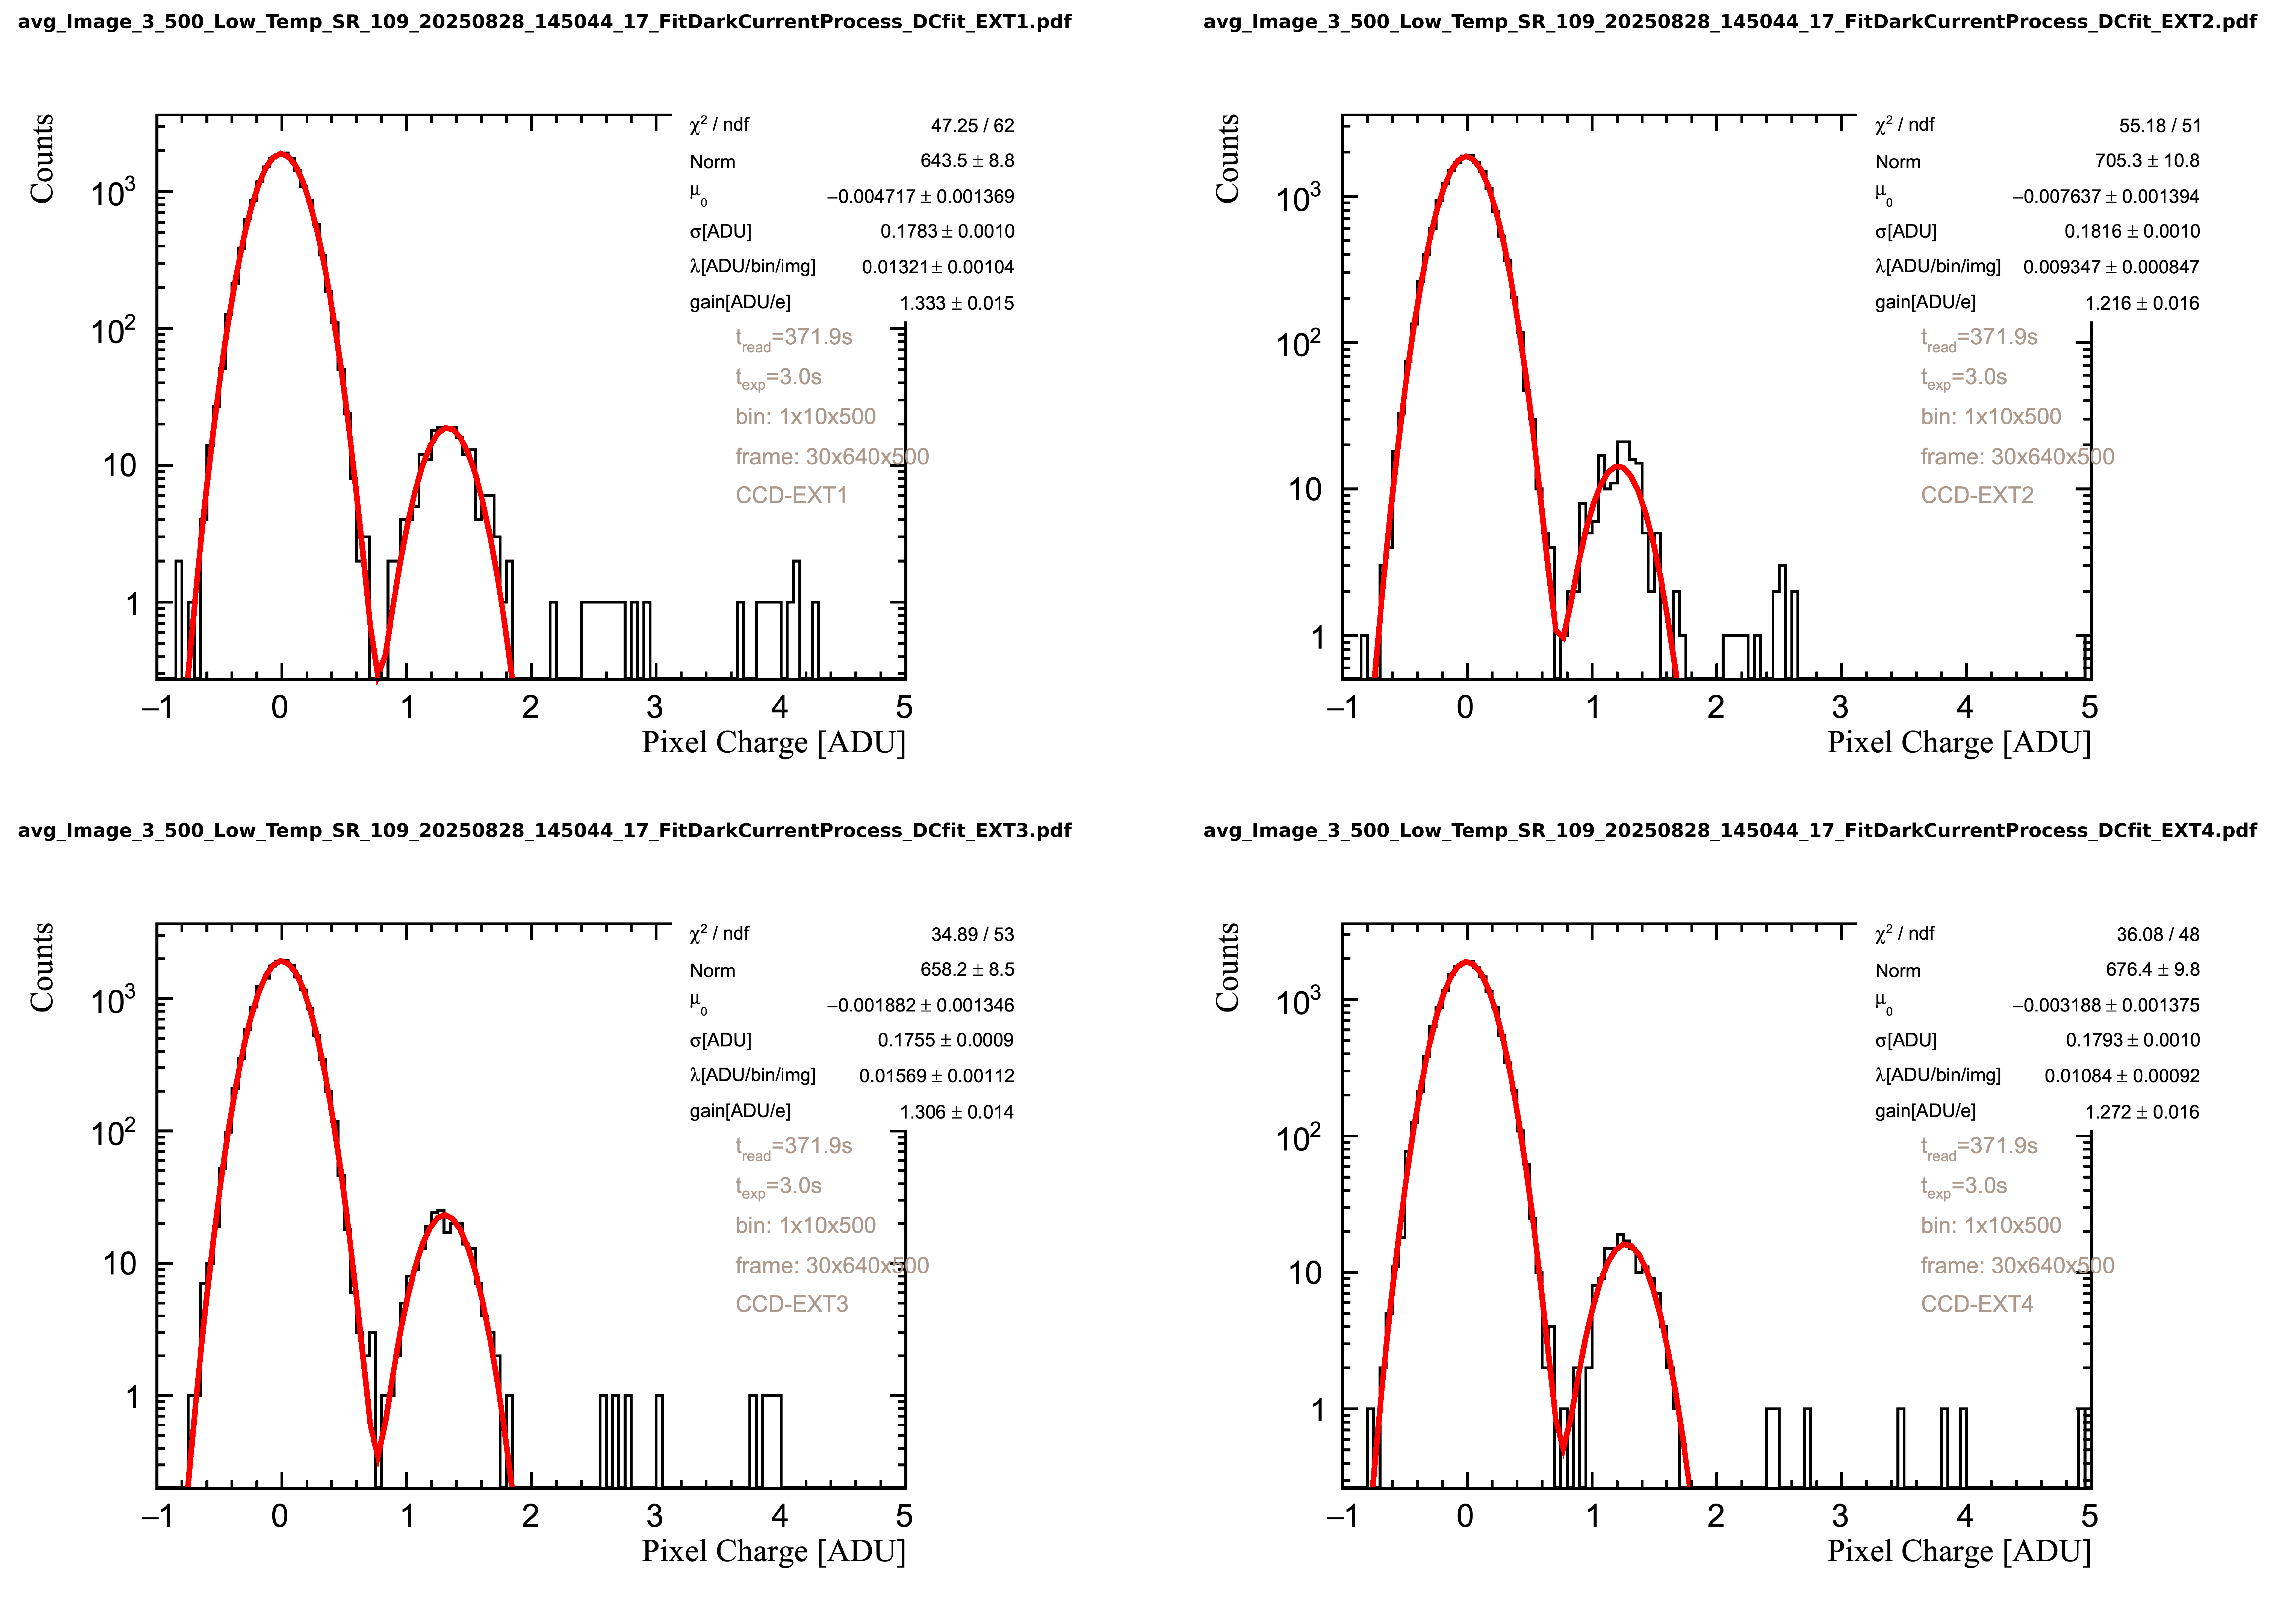
\includegraphics[width=1\linewidth]{figures/DM09_Image_31_Low.png}
    \caption[Composite image analysis]{Pixel charge distributions (averaged over 500 NDCMs) for the four CCD extensions (EXT1–EXT4) of module DM-09 at 135\,K, obtained from \texttt{Image\_3\_135}. The red curves show fits to a Poisson distribution convolved with a Gaussian. The spacing between consecutive peaks provides the amplifier gain (in ADU/$e^-$), while the peak width corresponds to the resolution ($\sigma$). The fitted Poisson parameter $\lambda$ represents the average collected charge per pixel, associated with serial register dark current and clock-induced charge.
    }
    \label{fig:DM09_SE_fits}
\end{figure}
The skipper performance metrics extracted from the Poisson–Gaussian fits to the \texttt{Image\_3\_135} data are summarized in Figs.~\ref{fig:Single_e_res_all}--\ref{fig:DC_all}: the single-electron resolution ($\sigma$) derived from the Gaussian width of the fitted charge peaks, the amplifier gain obtained from the spacing between consecutive peaks, and the dark current inferred from the fitted Poisson rate parameter $\lambda$ (converted to $e^-$/pixel/day), each shown for all four CCD extensions (A–D) across modules DM-01 to DM-28. In each figure, the dotted horizontal line indicates the mean value across all extensions, and the shaded band represents $\pm 1\sigma$ about the mean.

\begin{figure}[H]
    \centering
    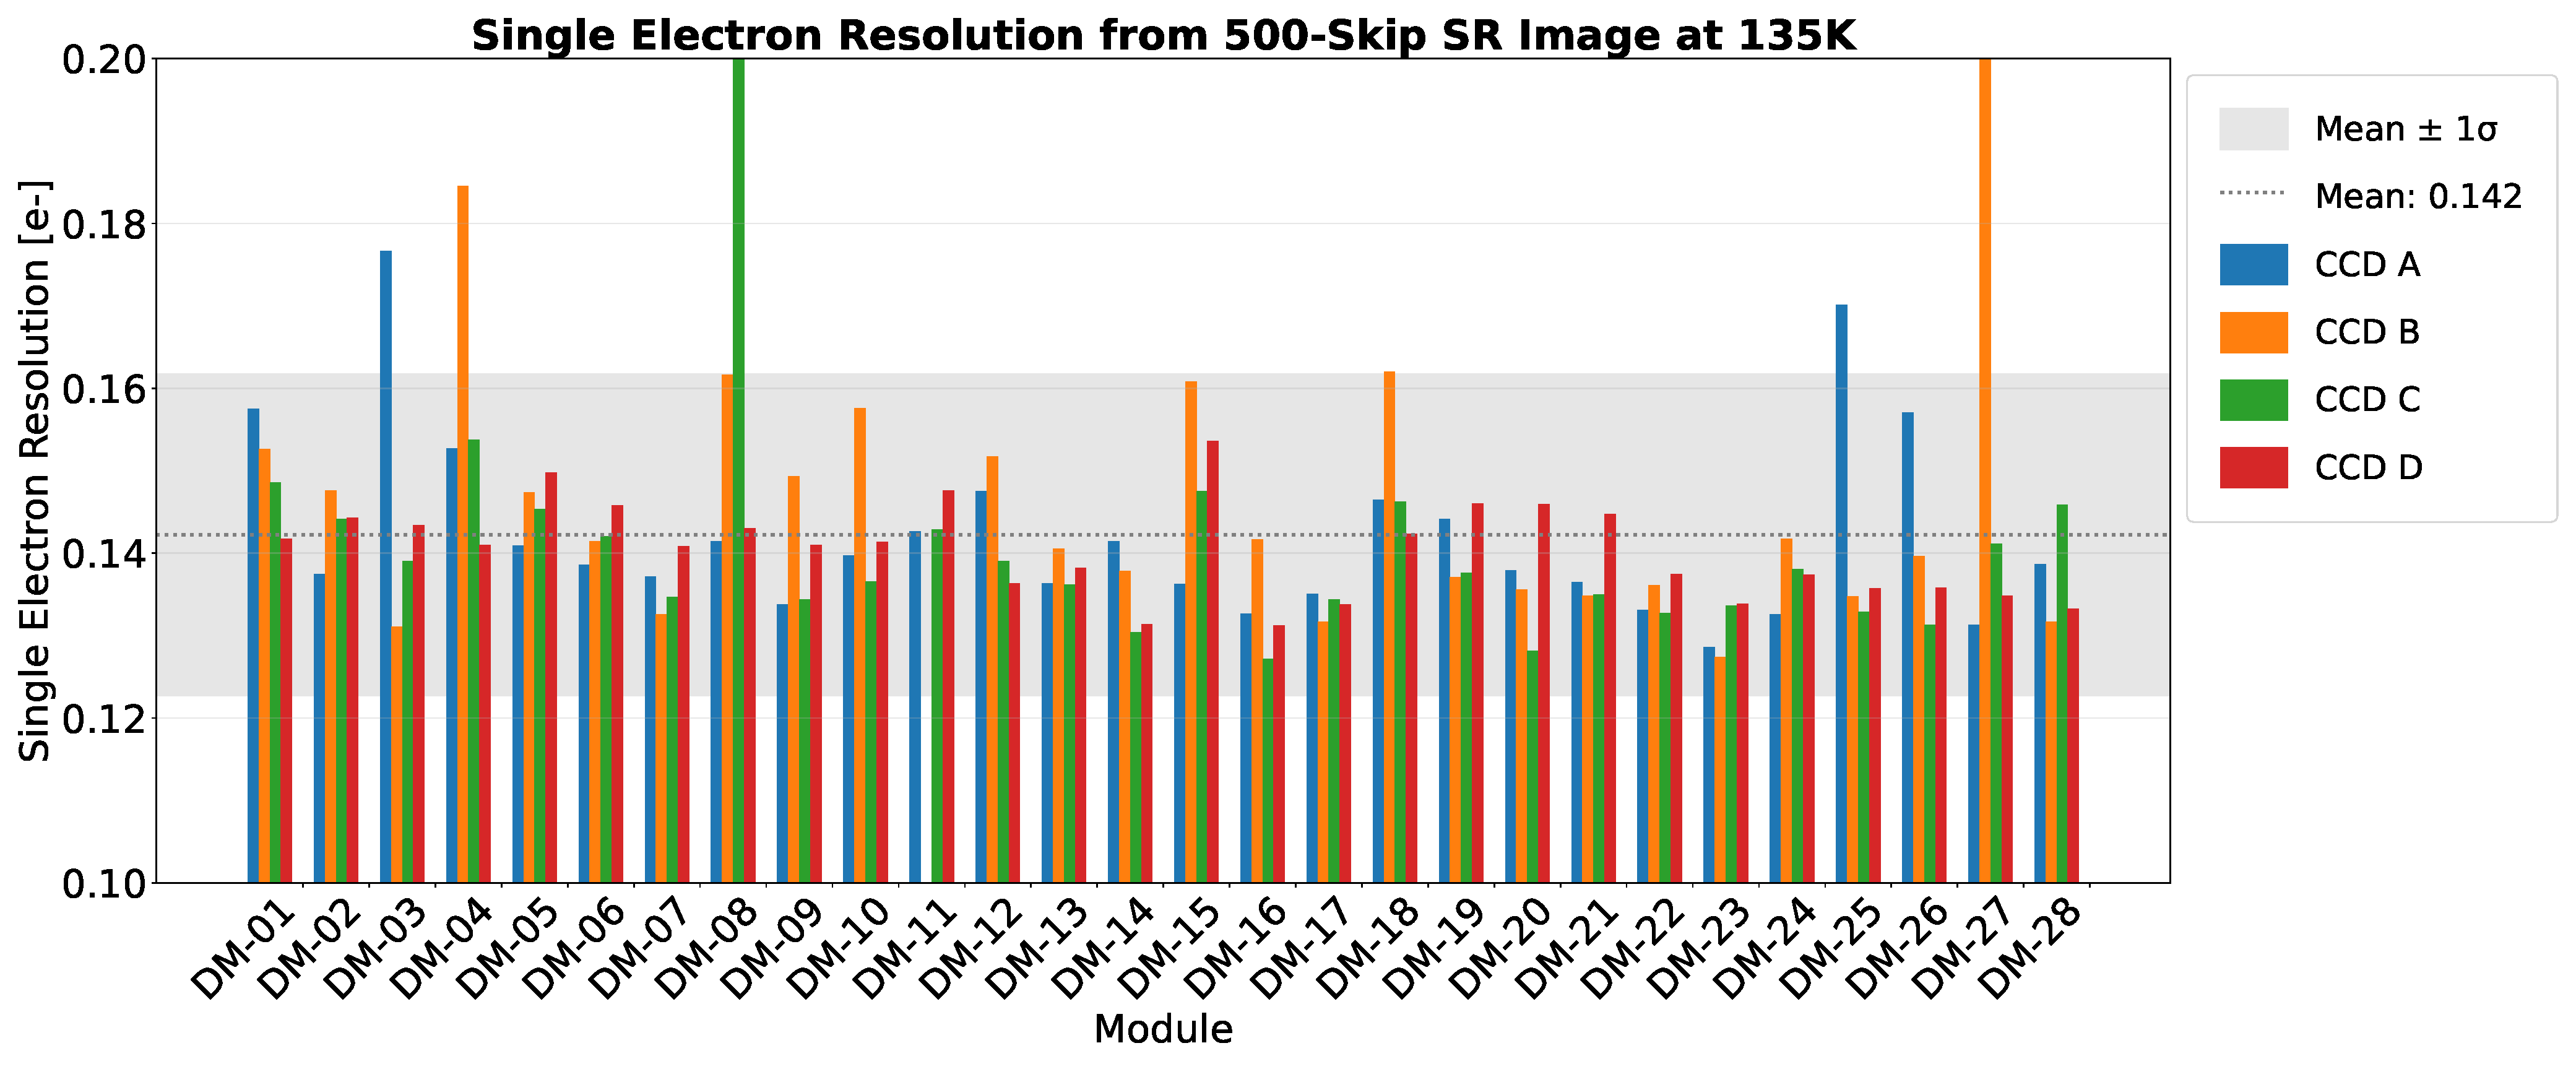
\includegraphics[width=1\linewidth]{figures/image31_low_res_all_modules.pdf}
    \caption[Single-electron resolution, all modules]{Single-electron resolution ($\sigma$) from the Poisson-convolved-Gaussian fit to \texttt{Image\_3\_135}, for each CCD extension (A--D) across modules DM-01 to DM-28. The dotted line and shaded band indicate the ensemble mean ($0.142\,e^-$) and $\pm1\sigma$ band.}
    \label{fig:Single_e_res_all}
\end{figure}

The single-electron resolution is tightly clustered around the ensemble mean of $0.142\,e^-$, with the majority of extensions falling within the $\pm1\sigma$ band (roughly $0.12$--$0.16\,e^-$). A handful of extensions in DM-03, DM-04, and DM-25 lie modestly above this band ($0.17$--$0.18\,e^-$), while DM-08 and DM-27 each contain one extension exceeding $0.20\,e^-$, the most significant single-electron-resolution outliers in the dataset.

\begin{figure}[H]
    \centering
    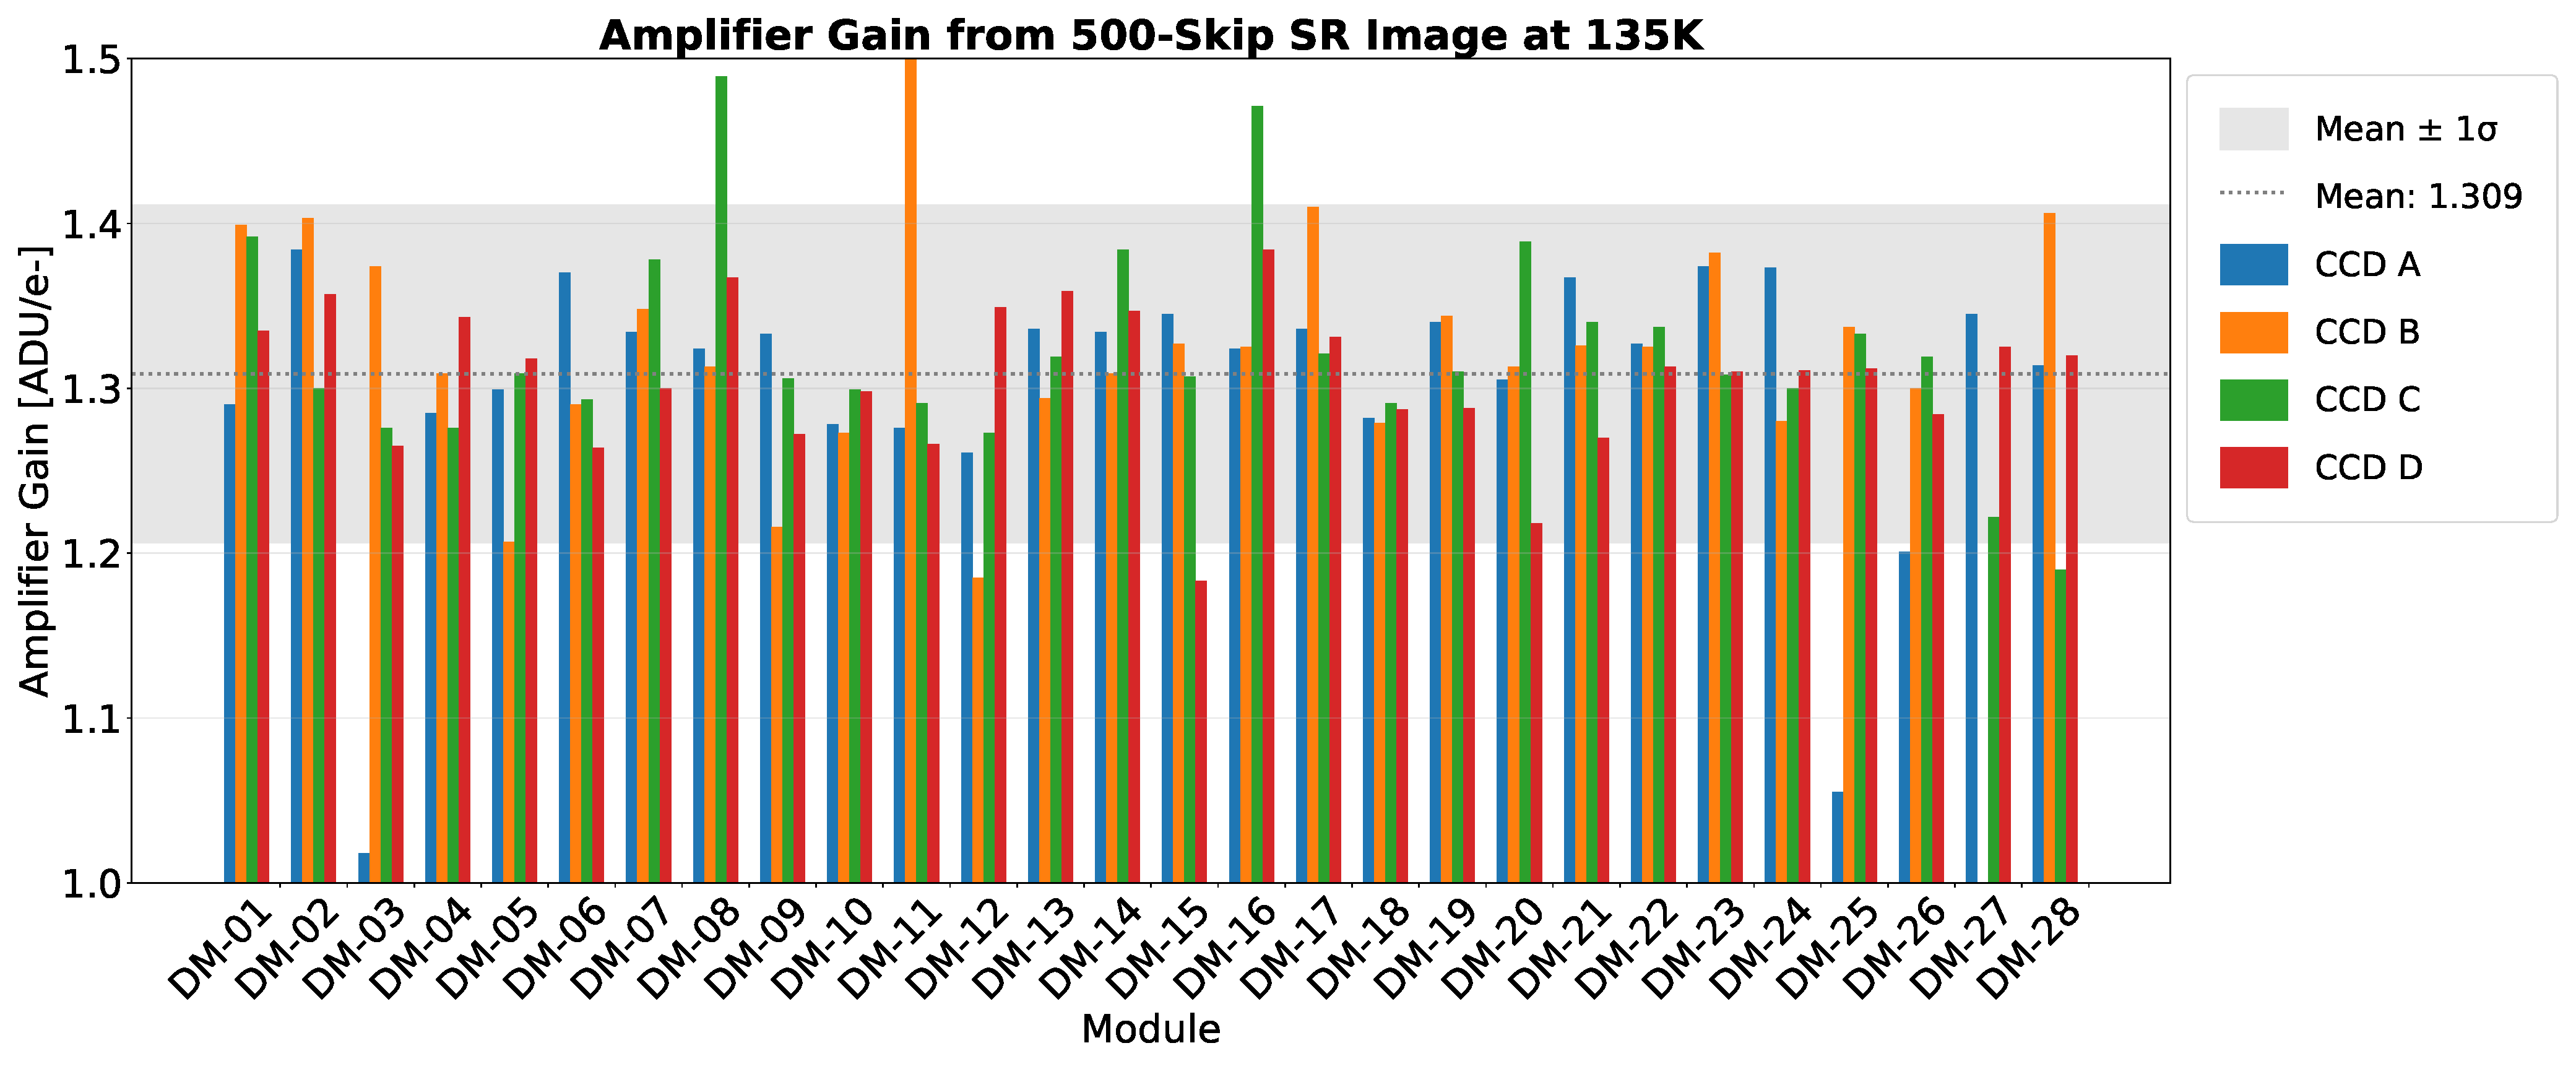
\includegraphics[width=1\linewidth]{figures/image31_low_gain_all_modules.pdf}
    \caption[Amplifier gain, all modules]{Amplifier gain from the Poisson-convolved-Gaussian fit to \texttt{Image\_3\_135}, for each CCD extension (A--D) across modules DM-01 to DM-28. The dotted line and shaded band indicate the ensemble mean ($1.308$\,ADU/$e^-$) and $\pm1\sigma$ band.}
    \label{fig:Gain_all}
\end{figure}

Amplifier gain is more broadly distributed than the resolution, with most extensions falling between $1.2$ and $1.4$\,ADU/$e^-$, centered on the ensemble mean of $1.308$\,ADU/$e^-$. DM-03 and DM-25 each contain one extension with anomalously low gain (near $1.0$--$1.06$\,ADU/$e^-$), while DM-08, DM-11, and DM-16 each contain one extension approaching or exceeding $1.45$\,ADU/$e^-$, the highest values in the dataset.

\begin{figure}[H]
    \centering
    \includegraphics[width=1\linewidth]{figures/image31_low_dark_current_all_modules.pdf}
    \caption[Dark current at 135\,K, all modules]{Dark current at 135\,K, inferred from the fitted Poisson rate parameter $\lambda$ of \texttt{Image\_3\_135} and converted to $e^-$/pixel/day, for each CCD extension (A--D) across modules DM-01 to DM-28. The dotted line and shaded band indicate the ensemble mean ($0.388\,e^-$/pix/day) and $\pm1\sigma$ band.}
    \label{fig:DC_all}
\end{figure}

The dark-current distribution at 135\,K is strongly skewed by a small number of modules well above the ensemble mean of $0.388\,e^-$/pix/day. DM-08 is the most extreme outlier, exceeding $10\,e^-$/pix/day in two extensions, consistent with the large column defect described in Sec.~\ref{sec:column_defects} that produces amplifier glow in that module. DM-10 and DM-12 are the next-highest modules, at roughly $3$ and $1$--$1.4\,e^-$/pix/day, respectively. DM-24, DM-25, and DM-26 are also elevated relative to the ensemble mean, consistent with the installation-related dark-current increase noted in the Executive Summary (Sec.~\ref{sec:summary}).

For comparison, Fig.~\ref{fig:DC_high_all} shows the same dark-current measurement repeated at 185\,K (\texttt{Image\_4\_185}), and Fig.~\ref{fig:DC_ratio_all} shows the ratio of the 135\,K to 185\,K dark current for each extension. The ratio quantifies the temperature dependence of the dark current per extension and is a useful diagnostic for identifying extensions whose dark current does not follow the expected thermal-activation behavior.

\begin{figure}[H]
    \centering
    \includegraphics[width=1\linewidth]{figures/image31_high_dark_current_all_modules.pdf}
    \caption[Dark current at 185\,K, all modules]{Dark current at 185\,K, inferred analogously to Fig.~\ref{fig:DC_all} but from \texttt{Image\_4\_185}, for each CCD extension (A--D) across modules DM-01 to DM-28. The ensemble mean is $131.1\,e^-$/pix/day, roughly $340\times$ the 135\,K value, consistent with the expected thermal activation of dark current.}
    \label{fig:DC_high_all}
\end{figure}

At 185\,K the dark-current distribution is markedly more uniform than at 135\,K: nearly all extensions fall within a factor of a few of the ensemble mean of $131.1\,e^-$/pix/day, and none approach the order-of-magnitude excursions seen at 135\,K. The only modules that stand out are DM-21, DM-22, and DM-23, whose extensions reach roughly $200$--$350\,e^-$/pix/day, moderately above the $\pm1\sigma$ band. Notably, these are not the same modules that dominate the 135\,K distribution (DM-08, DM-10, DM-12), suggesting that the anomalous 135\,K dark current in those modules is not a purely thermally-activated bulk effect.

\begin{figure}[H]
    \centering
    \includegraphics[width=1\linewidth]{figures/image31_ratio_low_high_dark_current_all_modules_underground.pdf}
    \caption[Ratio of 135\,K to 185\,K dark current, all modules]{Ratio of the 135\,K to 185\,K dark current (Fig.~\ref{fig:DC_all} over Fig.~\ref{fig:DC_high_all}) for each CCD extension (A--D) across modules DM-01 to DM-28, on a logarithmic scale. The ensemble mean ratio is $3.0\times10^{-3}$. \todonote{We still need an unclipped version of this plot for the final report, since several ratios exceed the $10^{-2}$ y-axis cap.}}
    \label{fig:DC_ratio_all}
\end{figure}

The ratio highlights the same modules identified as 135\,K dark-current outliers -- DM-08, DM-10, DM-12, and DM-24--DM-26 -- as having anomalously high 135-to-185\,K ratios, several of which exceed the $10^{-2}$ clipping threshold of the source plot. This is consistent with the 135\,K excess in these modules arising from a mechanism (e.g.\ surface- or defect-related leakage) that does not scale with temperature the way the bulk thermally activated dark current dominating the 185\,K measurement does.


\subsection{Fe-55 events}

X-rays from the radioactive decay of $^{55}$Fe in the iron foils attached to the storage box lids (module packaging described in \cite{Traina2025}) produce ionization events throughout the CCD bulk, including both front- and back-side interactions.
Fig.~\ref{fig:fe55foilphoto} shows the foils as mounted on a pair of module storage-box lids, each covering a narrow strip of the CCD active area.
These monoenergetic X-rays provide a controlled probe of the detector response and are used to characterize the keV-scale energy calibration, charge transfer inefficiency (CTI), lateral charge diffusion, and cross-talk in the sensors~\cite{Janesick:2001}.

\begin{figure}[H]
    \centering
    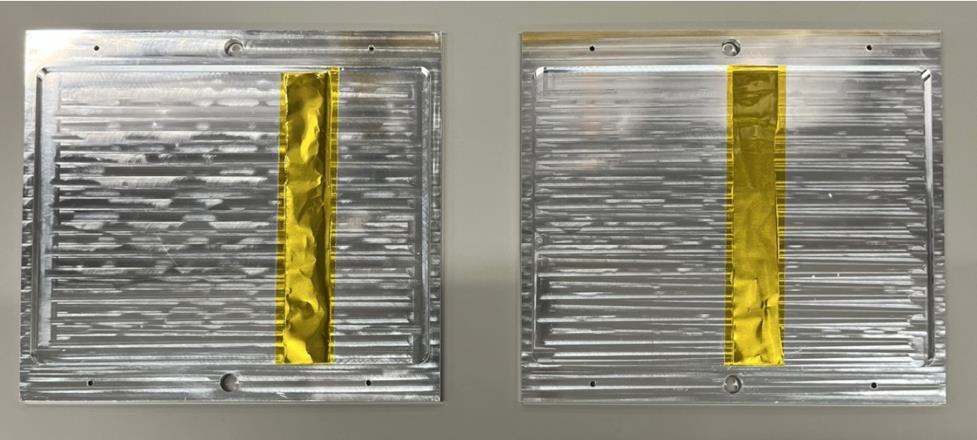
\includegraphics[width=0.85\linewidth]{figures/fe55_foil_photo.png}
    \caption[Iron-55 foil mounting]{The two $^{55}$Fe foils (yellow strips) mounted on module storage-box lids, positioned over a narrow column of the CCD active area to provide a localized source of monoenergetic X-rays for calibration.}
    \label{fig:fe55foilphoto}
\end{figure}

Images are processed by identifying contiguous pixels above background noise and grouping them into reconstructed ``clusters,'' using a seed threshold of $\sim$7\,$e^-$ and a pixel-inclusion threshold of $\sim$2\,$e^-$.
For each cluster, the sum of the pixel values is proportional to the deposited energy, while the charge-weighted mean and standard deviation of the pixel coordinates provide estimates of the interaction position and transverse charge spread, respectively.
The lateral spread, quantified by $\sigma_{xy}$, is positively correlated with the interaction depth in the silicon bulk. Charge generated near the pixel array (front-side events) is collected after only a short drift through the depleted silicon, so lateral diffusion has little time to act and the resulting clusters are compact, with small $\sigma_{xy}$. Charge generated near the back surface, in contrast, must drift over the full thickness of the depleted bulk before collection; the longer drift time allows lateral diffusion to spread the charge over a larger area, producing more diffuse clusters with larger $\sigma_{xy}$. This depth-dependent diffusion is the same effect used to separate the front- and back-side populations in Fig.~\ref{fig:ironfoil}.

The top panel of Fig.~\ref{fig:ironfoil} shows a scatter plot of $\sigma_{xy}$ versus the $x$-coordinate for clusters with reconstructed energies between 4.5 and 7.0\,keV, calibrated using the amplifier gain. 
These events consist predominantly of $^{55}$Fe X-rays originating from the iron foils. 
Two clearly separated populations are observed, corresponding to front- and back-side interactions. 
The displacement of these populations along the $x$-axis reflects the physical placement of the iron foils above specific regions of the CCD. 
The bottom panel of Fig.~\ref{fig:ironfoil} presents the energy spectrum of front-side clusters selected with $\sigma_{xy}<1$\,pixel. 
Because front-side events deposit their charge over fewer pixels, they exhibit a higher signal-to-noise ratio and therefore a cleaner spectral structure.

It is important to distinguish between the surface and underground analyses of the $^{55}$Fe data. 
The scatter plot in Fig.~\ref{fig:ironfoil} corresponds to on-surface tests performed with full-array single-skip images, which were used to identify the spatial distribution of the Fe-55 events and validate the depth-based separation via $\sigma_{xy}$. 
For the underground low-temperature characterization at LSM (135\,K), a dedicated acquisition strategy was adopted. 
In particular, Image\_5 was selected: a cropped region of 1280 columns by 480 rows, centered on the area illuminated by the iron foils and read out with 500 skips.
This configuration enhances the signal-to-noise ratio and enables high-resolution measurements of the energy response and CTI-sensitive cluster morphology in the region of interest. As shown in the top panel of Fig.~\ref{fig:ironfoil}, the Image\_5 crop region (1280 columns $\times$ 480 rows) is centered on the boundary between the front- and back-side populations used in the underground analysis.

In the following subsections, the underground cropped multi-skip data are used to (i) validate the keV-scale energy calibration and resolution at operating temperature, and (ii) perform CTI-sensitive studies based on composite-cluster morphology and charge asymmetry diagnostics.

\begin{figure}[H]
    \centering
    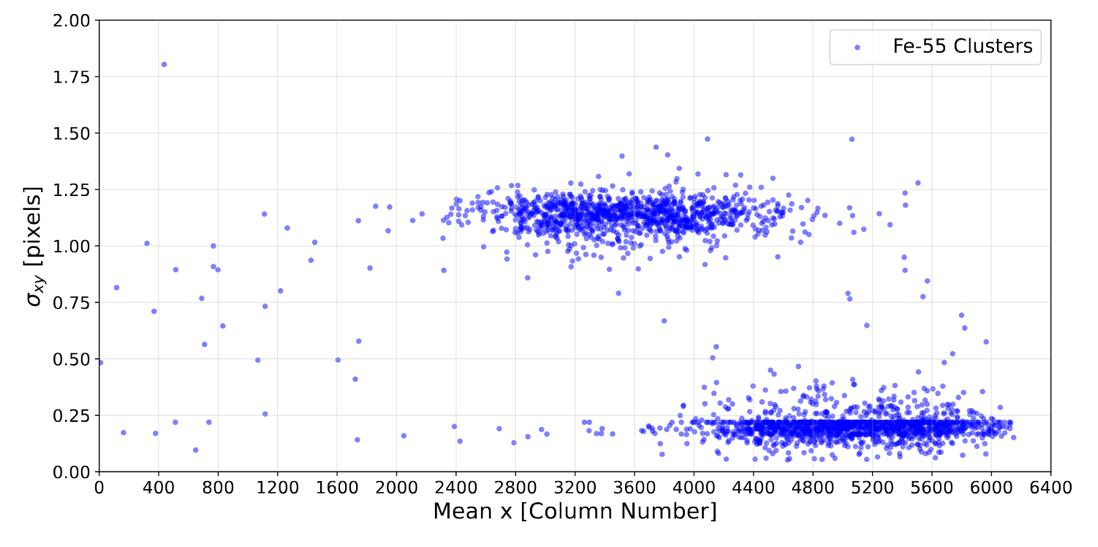
\includegraphics[width=0.85\linewidth]{figures/ironfoil_sigma_xy_scatter.png}\\[0.5em]
    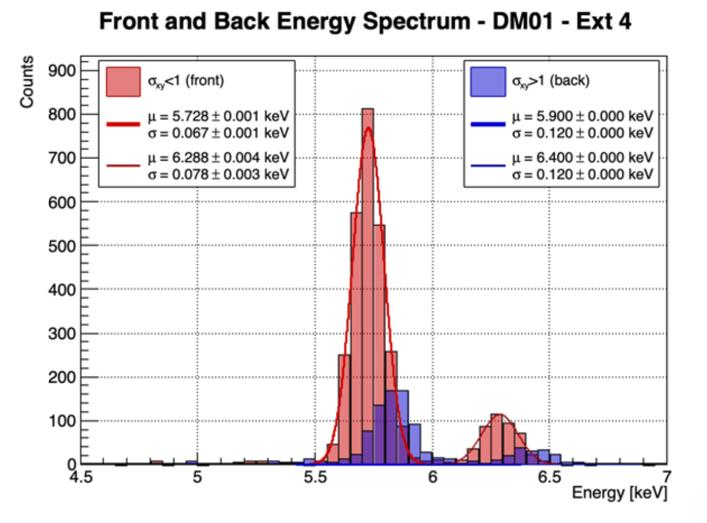
\includegraphics[width=0.85\linewidth]{figures/ironfoil_energy_spectrum.png}
    \caption[Fe-55 event separation and energy spectrum]{\textit{Top:} scatter plot of the cluster lateral spread $\sigma_{xy}$ versus mean $x$-coordinate for $^{55}$Fe clusters with reconstructed energy between 4.5 and 7.0\,keV, from an on-surface full-array single-skip dataset. Two populations are visible, separated by $\sigma_{xy}$: a compact, low-$\sigma_{xy}$ front-side population and a more diffuse, high-$\sigma_{xy}$ back-side population, each localized in $x$ to the physical footprint of the iron foils mounted on the module lids. \textit{Bottom:} reconstructed energy spectrum for the same dataset, split into front-side ($\sigma_{xy}<1$\,pixel, red) and back-side ($\sigma_{xy}>1$\,pixel, blue) populations, for a representative extension (DM01, Ext.\ 4). The front-side spectrum resolves the Mn K$\alpha$ (5.9\,keV) and K$\beta$ (6.49\,keV) lines with substantially better resolution than the back-side spectrum, consistent with the shorter drift path and reduced diffusion for front-side events.}
    \label{fig:ironfoil}
\end{figure}

\subsection{Charge Transfer Inefficiency (CTI) Studies}
\label{sec:CTI}

Charge transfer inefficiency (CTI) manifests as charge loss and trailing during pixel-to-pixel transfer toward the readout registers. 
In this analysis, CTI is probed using morphological diagnostics derived from averaged $^{55}$Fe clusters. 
Rather than extracting a per-transfer CTI coefficient, the procedure evaluates directional asymmetries and tail properties of composite clusters that are sensitive to charge-trailing effects.

\subsubsection*{Composite Cluster Construction}

For each selected $^{55}$Fe cluster in the 4.5--7.0\,keV window, a two-dimensional pixel map is constructed using the per-cluster pixel lists (\texttt{pixels\_x}, \texttt{pixels\_y}, \texttt{pixels\_E}). 
The cluster is then recentered in relative coordinates according to

\begin{equation}
(\Delta x, \Delta y) = (x - x_{\mathrm{centroid}}, y - y_{\mathrm{centroid}}),
\end{equation}

where $(x_{\mathrm{centroid}}, y_{\mathrm{centroid}})$ denotes the charge-weighted cluster position. 
The charge distribution is accumulated on a fixed grid spanning

\begin{equation}
-4~\text{pixels} < \Delta x, \Delta y < 4~\text{pixels}.
\end{equation}

After processing all clusters, the composite image is normalized by the total number of events,

\begin{equation}
C_{\mathrm{composite}}(\Delta x, \Delta y)
=
\frac{1}{N}
\sum_{k=1}^{N}
C_k(\Delta x, \Delta y),
\end{equation}

yielding the average cluster morphology. 
Separate composite images are constructed for front- and back-side populations defined via the $\sigma_{xy}$ discriminator.

In the composite-cluster coordinate system, $\Delta x$ corresponds to the horizontal pixel direction (CCD columns), while $\Delta y$ corresponds to the vertical pixel direction (CCD rows). 
These axes map directly onto the CCD readout directions: charge is transferred vertically through the pixel array during the parallel transfer stage and horizontally through the serial register during readout.

\subsubsection*{Front-Side CTI Diagnostics}

For the front-side composite, the average cluster is divided into a central region and four neighboring regions that probe charge extending away from the cluster core along the two CCD transfer directions. 
The central region is defined as the $1\times1$ pixel box centered on the cluster centroid,

\begin{equation}
|\Delta x| < 0.5, \qquad |\Delta y| < 0.5,
\end{equation}

and contains the core of the average front-side cluster.

To quantify charge asymmetries around this core, four adjacent regions are defined:

\begin{itemize}
\item \textbf{Above:} region located at positive $\Delta y$, probing charge extending upward from the cluster core.
\item \textbf{Below:} region located at negative $\Delta y$, probing charge extending downward from the cluster core.
\item \textbf{Right:} region located at positive $\Delta x$, probing charge extending to the right of the cluster core.
\item \textbf{Left:} region located at negative $\Delta x$, probing charge extending to the left of the cluster core.
\end{itemize}

Fig.~\ref{fig:front_composite_example} shows an example composite cluster illustrating these regions.
The colored boxes indicate the areas used to evaluate the directional charge fractions.

\begin{figure}[H]
    \centering
    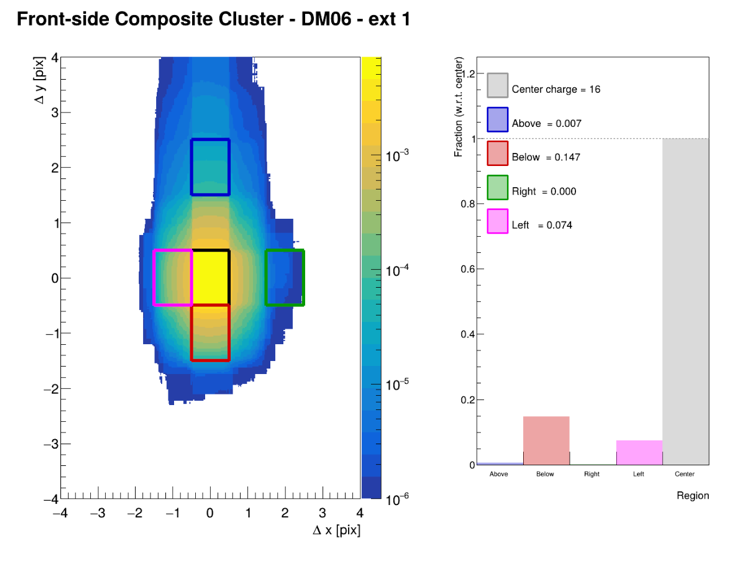
\includegraphics[width=0.95\linewidth]{figures/front_composite_example_DM06.png}
    \caption[Front-side composite cluster example]{Front-side composite $^{55}$Fe cluster for DM06, Ext.\ 1, in relative coordinates $(\Delta x, \Delta y)$ (left), and the corresponding integrated charge fractions in the Above, Below, Left, and Right regions, normalized to the central region (right). This module is chosen as the illustrative example because it exhibits a particularly clear parallel (vertical) CTI signature: the Below fraction (0.147) noticeably exceeds the Above fraction (0.007), indicating charge trailing along the parallel (row) transfer direction, while the Left/Right (serial) asymmetry is comparatively small (0.074 vs.\ 0.000).}
    \label{fig:front_composite_example}
\end{figure}

In the implementation, these regions are evaluated by integrating the composite cluster over fixed rectangular windows in $(\Delta x,\Delta y)$ around the core. 
The corresponding integrated charges, $Q_{\mathrm{region}}$, are then normalized to the charge in the central region, $Q_{\mathrm{center}}$, according to

\begin{equation}
f_{\mathrm{region}} =
\frac{Q_{\mathrm{region}}}{Q_{\mathrm{center}}}
\end{equation}

In the absence of directional charge trailing, opposite regions are expected to be comparable,

\begin{equation}
f_{\mathrm{Above}} \approx f_{\mathrm{Below}}, 
\qquad
f_{\mathrm{Left}} \approx f_{\mathrm{Right}}.
\end{equation}

Systematic differences between opposite regions indicate preferential charge redistribution in one direction, consistent with asymmetric transfer effects.
In practice, two quantities derived from these regional fractions are used as compact CTI-sensitive observables,

\begin{equation}
f_{\mathrm{Above}} =
\frac{Q_{\mathrm{Above}}}{Q_{\mathrm{center}}},
\qquad
f_{\mathrm{Right}} =
\frac{Q_{\mathrm{Right}}}{Q_{\mathrm{center}}}.
\end{equation}

The fraction $f_{\mathrm{Above}}$ probes charge redistribution along the parallel transfer direction, while $f_{\mathrm{Right}}$ probes redistribution along the serial transfer direction. 
These quantities are evaluated for each extension of every module and summarized in the figures below to provide a global comparison of CTI-sensitive charge redistribution across the detector ensemble.

\begin{figure}[H]
    \centering
    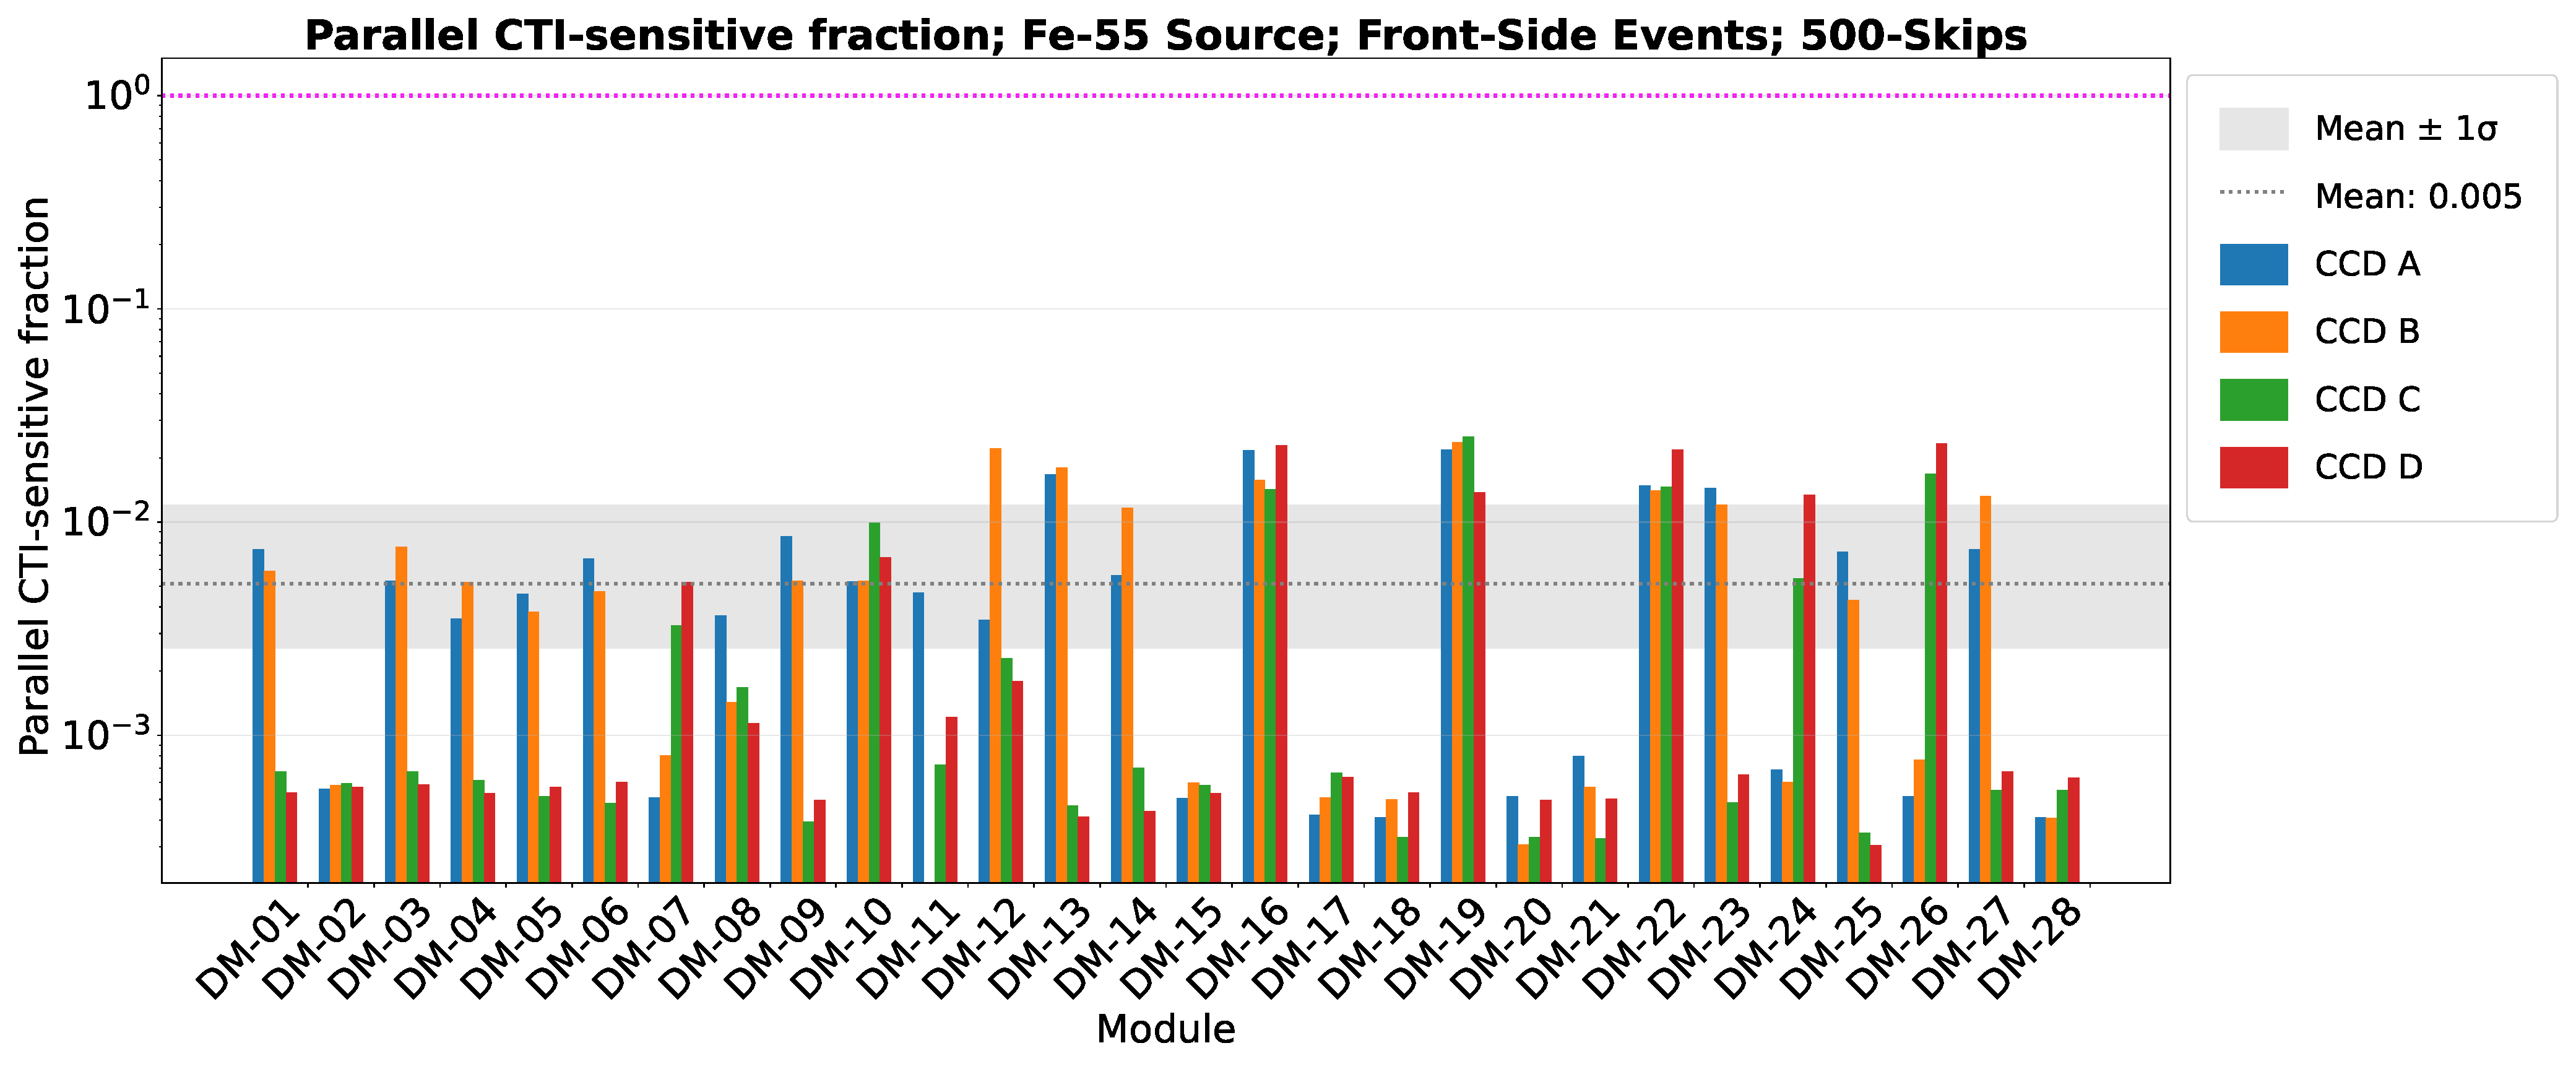
\includegraphics[width=1\linewidth]{figures/image5_low_cti_front_above_fraction_all_modules.pdf}
    \caption[Parallel CTI-sensitive fraction, all modules]{Parallel CTI-sensitive fraction $f_{\mathrm{Above}}$ from front-side $^{55}$Fe clusters (500-skip Image\_5 data), for each CCD extension (A--D) across modules DM-01 to DM-28. The dotted line and shaded band indicate the ensemble mean ($5\times10^{-3}$) and $\pm1\sigma$ band.}
    \label{fig:cti_front_above_all}
\end{figure}

The parallel CTI-sensitive fraction is tightly clustered near zero for most extensions, with the ensemble mean of $5\times10^{-3}$ pulled upward by a right-skewed tail. DM-16 and DM-19 are the most consistently elevated modules, with all four extensions above $10^{-2}$, roughly a factor of two to three above the ensemble mean. Several other modules -- DM-12, DM-13, DM-22, DM-23, and DM-26 -- each contain one or two extensions reaching similar levels, though without the module-wide consistency seen in DM-16 and DM-19.

\begin{figure}[H]
    \centering
    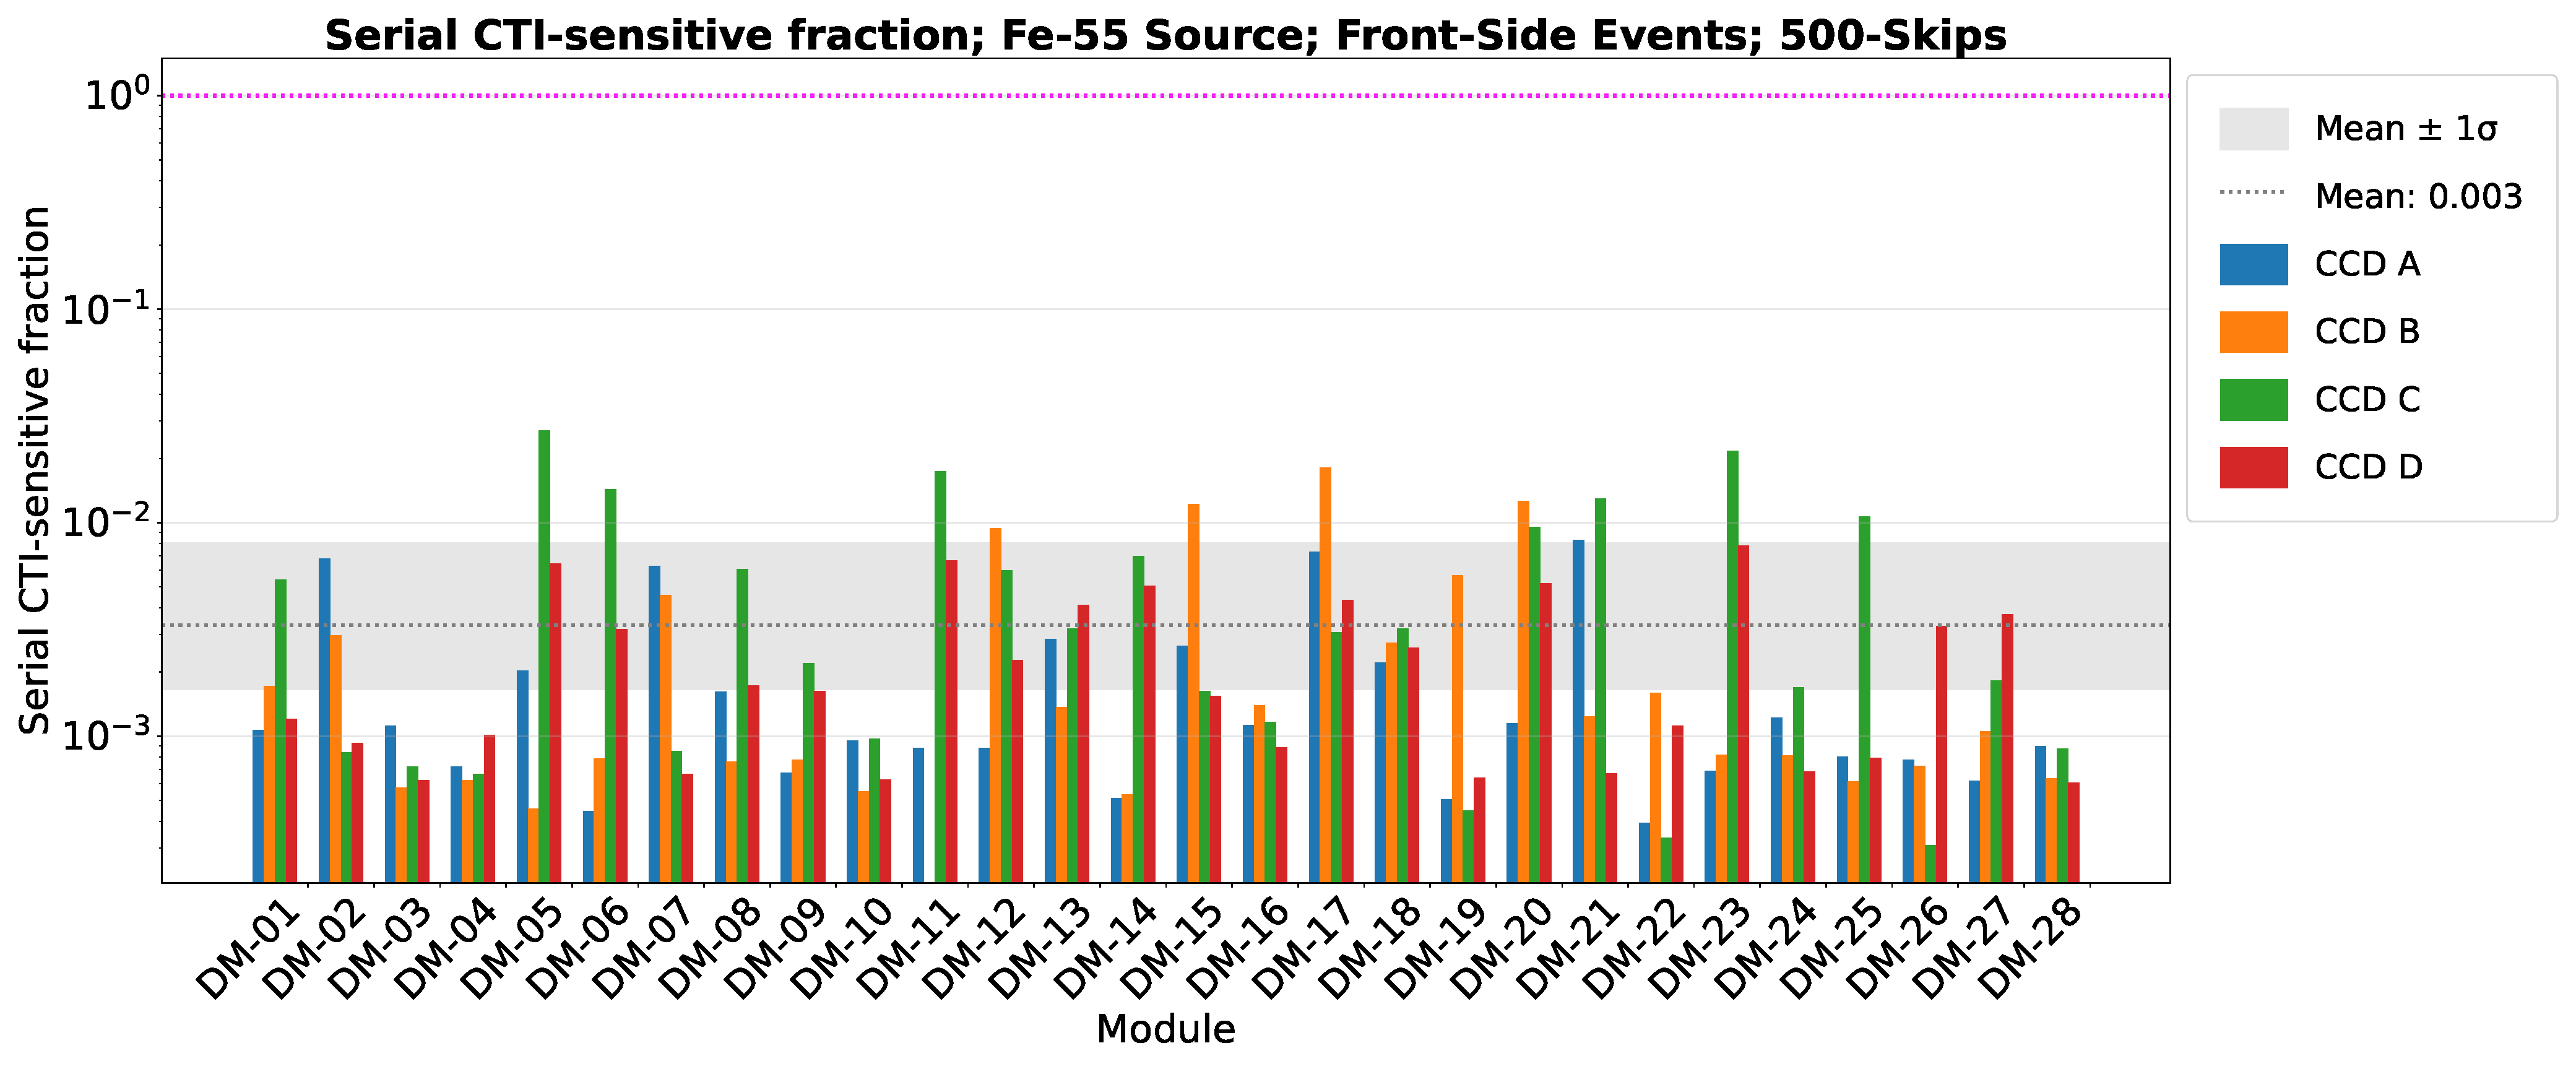
\includegraphics[width=1\linewidth]{figures/image5_low_cti_front_right_fraction_all_modules.pdf}
    \caption[Serial CTI-sensitive fraction, all modules]{Serial CTI-sensitive fraction $f_{\mathrm{Right}}$ from front-side $^{55}$Fe clusters (500-skip Image\_5 data), for each CCD extension (A--D) across modules DM-01 to DM-28. The dotted line and shaded band indicate the ensemble mean ($3\times10^{-3}$) and $\pm1\sigma$ band.}
    \label{fig:cti_front_right_all}
\end{figure}

The serial CTI-sensitive fraction is systematically smaller than its parallel counterpart (Fig.~\ref{fig:cti_front_above_all}), with an ensemble mean of $3\times10^{-3}$ and a comparatively narrow spread. Unlike the parallel fraction, no module shows a consistent elevation across all four extensions; the largest individual values, in DM-05, DM-11, DM-17, and DM-23, reach only about $2\times10^{-2}$ in a single extension each. This asymmetry between the parallel and serial fractions is consistent with the vertical (parallel-direction) CTI signature observed qualitatively across the module set, as noted in the Executive Summary (Sec.~\ref{sec:summary}).

\subsubsection*{Back-Side CTI Diagnostics}

Back-side events, which experience longer drift distances before reaching the pixel array, are particularly sensitive to charge-transport effects. 
For the back-side composite cluster, one-dimensional projections are constructed within fixed edge slabs of the composite grid to isolate the extended tails of the charge distribution.

From these projections, the following quantities are evaluated:

\begin{itemize}
\item Integrated charge (converted to electrons using 3.74\,eV per $e^{-}$),
\item Mean position,
\item RMS width,
\item Skewness.
\end{itemize}

The projection integrals probe the charge in extended tails, while the RMS and skewness quantify the width and directional asymmetry of the charge distribution. 
Because these quantities are derived from projections of the composite cluster, they characterize the systematic morphology of the average back-side event rather than the spread of individual clusters.

The RMS of the projections measures the width of the average back-side cluster distribution in each direction. 
Since lateral charge diffusion during the drift through the silicon bulk is expected to be approximately isotropic in the plane of the CCD, diffusion-dominated transport predicts similar RMS values for the serial and parallel projections. 
Significant deviations between the two directions would therefore indicate directional charge redistribution consistent with CTI effects or other transport asymmetries.

Figure~\ref{fig:back_composite_example} shows an illustrative example of a back-side composite cluster together with the projections used to evaluate these tail-sensitive observables.

\begin{figure}[H]
    \centering
    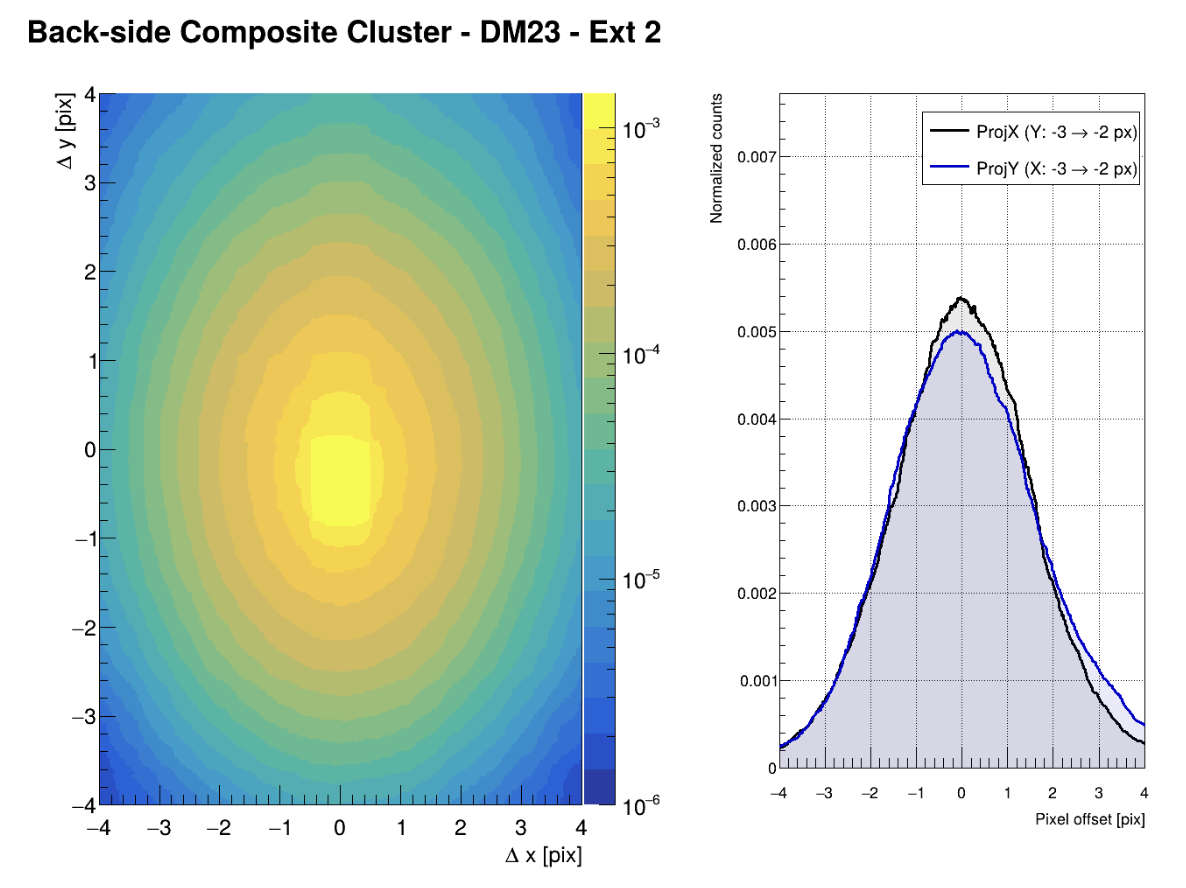
\includegraphics[width=0.95\linewidth]{figures/back_composite_example_DM23.png}
    \caption[Back-side composite cluster example]{Back-side composite $^{55}$Fe cluster for DM23, Ext.\ 2, in relative coordinates $(\Delta x, \Delta y)$ (left), and the corresponding one-dimensional serial (ProjX, black) and parallel (ProjY, blue) projections through the cluster core (right). The two projections are visually similar in width, consistent with isotropic diffusion dominating the back-side cluster shape for this example; the corresponding RMS widths for this module are summarized together with the full detector ensemble below.}
    \label{fig:back_composite_example}
\end{figure}

In addition to this example, summary plots of the RMS of the serial and parallel projections are produced for every extension of each module.
These plots provide a global comparison of the width of the back-side composite cluster tails across the detector ensemble.

\begin{figure}[H]
    \centering
    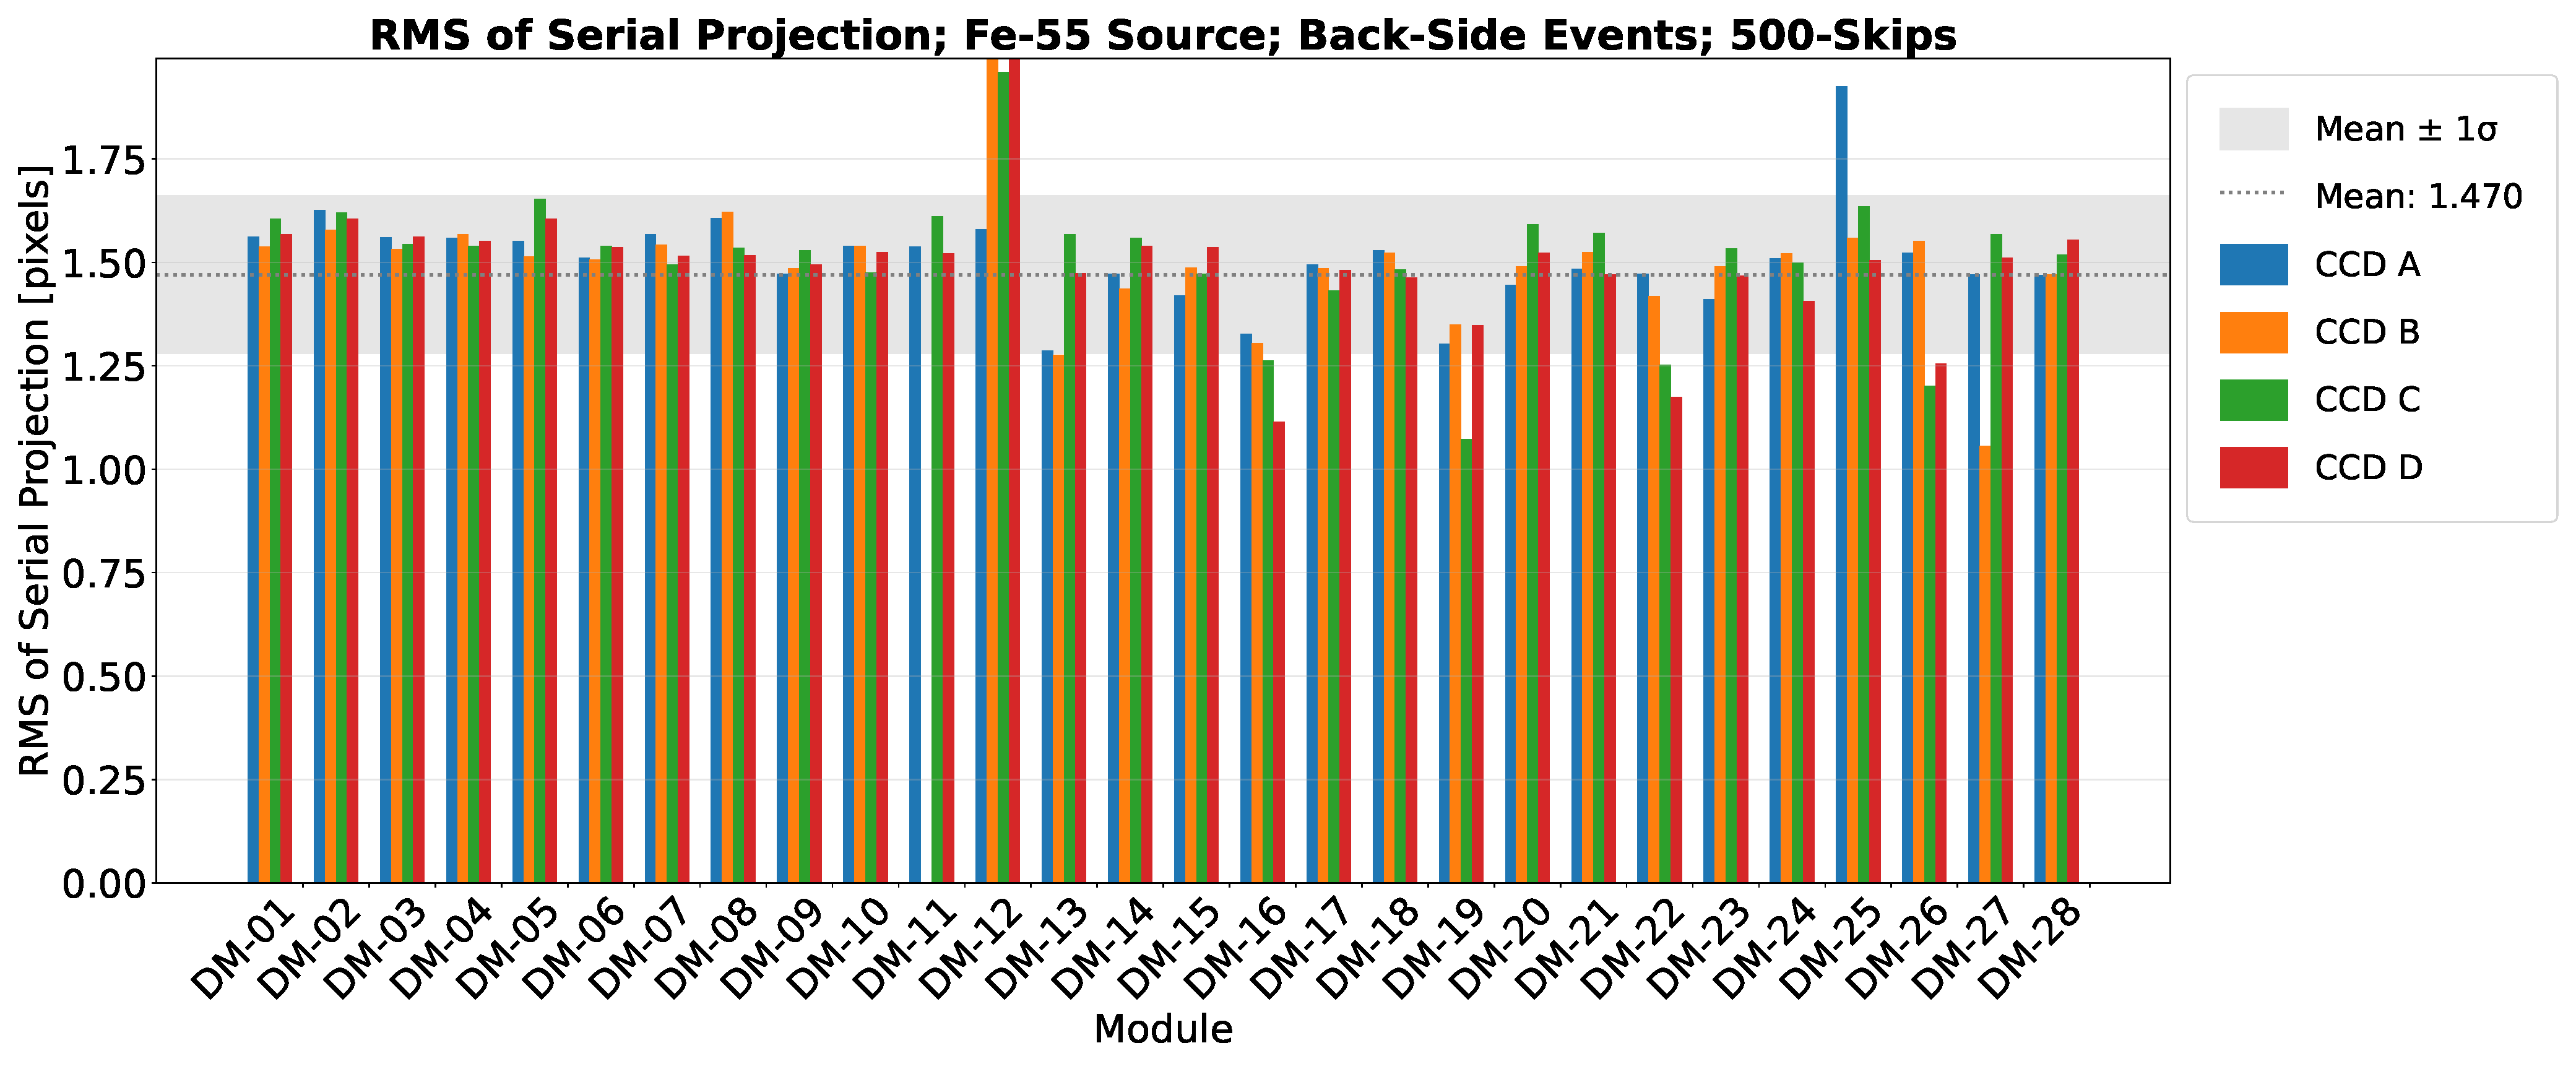
\includegraphics[width=1\linewidth]{figures/image5_low_cti_back_left_rms_all_modules.pdf}
    \caption[RMS of serial projection, back-side events, all modules]{RMS of the serial-direction ($\Delta x$) projection of the back-side composite $^{55}$Fe cluster, for each CCD extension (A--D) across modules DM-01 to DM-28. The dotted line and shaded band indicate the ensemble mean ($1.470$\,pixels) and $\pm1\sigma$ band.}
    \label{fig:cti_back_serial_rms_all}
\end{figure}

The RMS of the serial projection is narrowly distributed around the ensemble mean of $1.470$\,pixels for most modules, with two notable exceptions: DM-12 shows three extensions approaching or exceeding $2.0$\,pixels, and DM-25 shows one extension reaching $1.9$\,pixels, both well above the $\pm1\sigma$ band. A smaller number of modules -- DM-16, DM-19, DM-22, and DM-26 -- show mildly suppressed RMS values, in the $1.0$--$1.3$\,pixel range.

\begin{figure}[H]
    \centering
    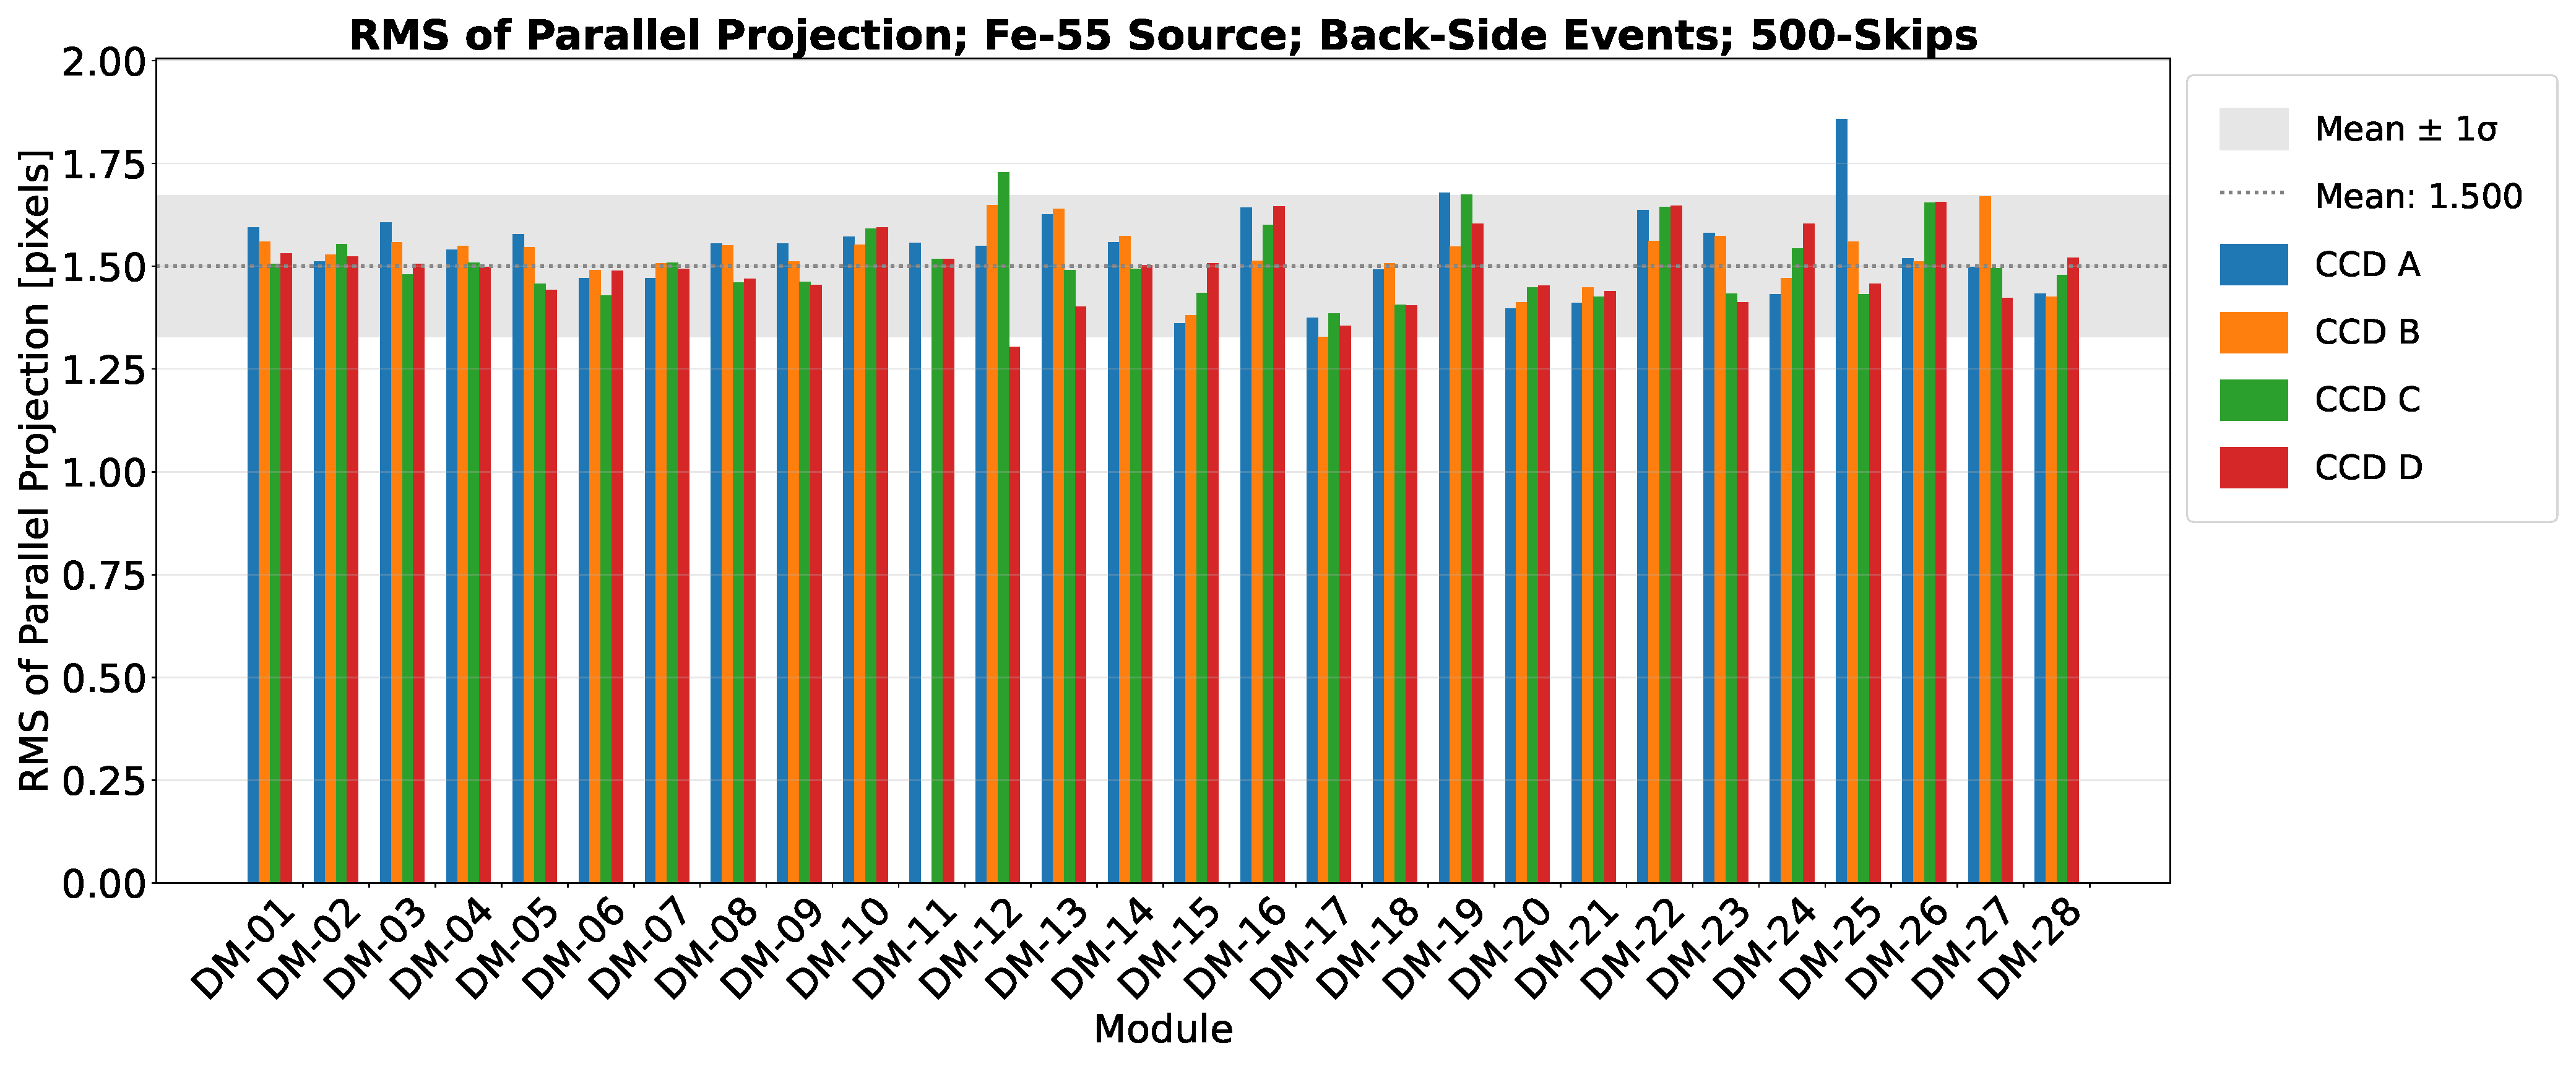
\includegraphics[width=1\linewidth]{figures/image5_low_cti_back_below_rms_all_modules.pdf}
    \caption[RMS of parallel projection, back-side events, all modules]{RMS of the parallel-direction ($\Delta y$) projection of the back-side composite $^{55}$Fe cluster, for each CCD extension (A--D) across modules DM-01 to DM-28. The dotted line and shaded band indicate the ensemble mean ($1.500$\,pixels) and $\pm1\sigma$ band.}
    \label{fig:cti_back_parallel_rms_all}
\end{figure}

The RMS of the parallel projection is more tightly distributed than the serial-direction RMS, closely matching the ensemble mean of $1.500$\,pixels for nearly every extension; only DM-25 stands out, with one extension reaching $1.86$\,pixels. Notably, DM-12, which showed the most extreme serial-direction RMS values in Fig.~\ref{fig:cti_back_serial_rms_all}, is unremarkable in the parallel direction ($\sim\!1.5$--$1.7$\,pixels). This directional asymmetry -- elevated serial RMS with normal parallel RMS -- is precisely the kind of deviation from isotropic diffusion described above, and identifies DM-12 as a candidate for closer inspection of serial-direction charge-transport effects.




\subsection{keV-scale calibration}
\label{sec:kev_calibration}

$^{55}$Fe decays produce two characteristic X-ray lines in the sensor, Mn K$\alpha$ (5.90\,keV) and Mn K$\beta$ (6.49\,keV), which provide an absolute keV-scale calibration of the pixel charge measured in electrons. Front-side events ($\sigma_{xy}<1$\,pixel, Sec.~\ref{sec:CTI}) are used for this calibration because their compact clusters yield a substantially better-resolved spectrum than the more diffuse back-side population (Fig.~\ref{fig:ironfoil}, bottom). Figure~\ref{fig:energy_vs_sigmaxy} shows this front/back separation directly in the energy-$\sigma_{xy}$ plane, for a representative extension (DM01, Ext.\ 4), at both the nominal LBC bias point and the revised $\mathrm{VR}=-6$\,V setting discussed below.

\begin{figure}[H]
    \centering
    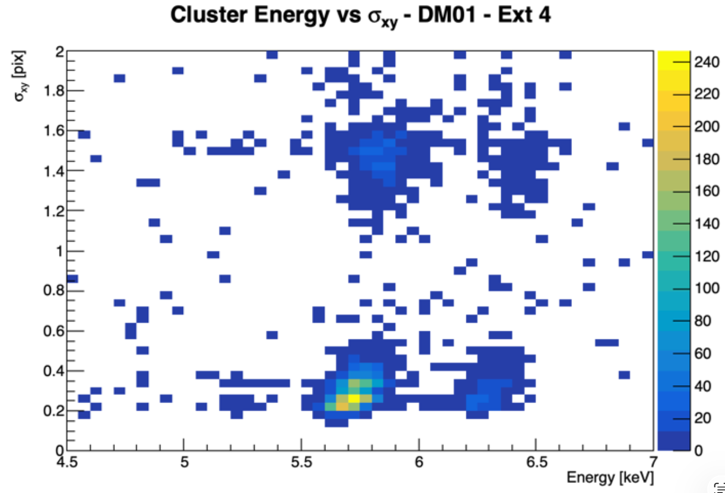
\includegraphics[width=0.48\linewidth]{figures/energy_vs_sigmaxy_VRm3V.png}
    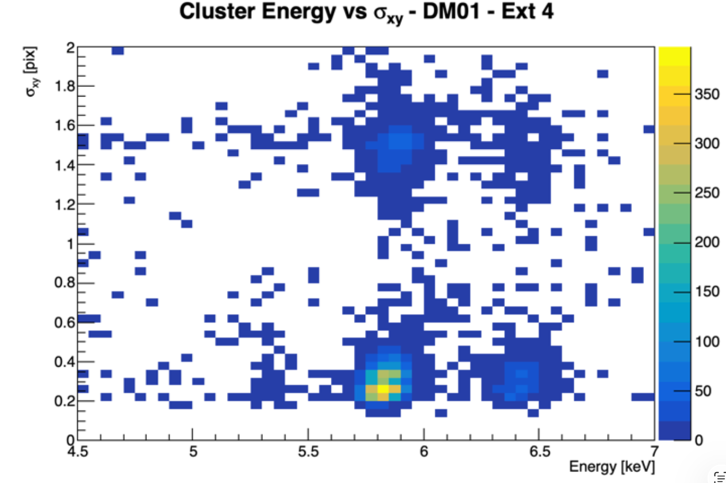
\includegraphics[width=0.48\linewidth]{figures/energy_vs_sigmaxy_VRm6V.png}
    \caption[Cluster energy vs.\ $\sigma_{xy}$, VR comparison]{Reconstructed cluster energy versus lateral spread $\sigma_{xy}$ for DM01, Ext.\ 4, at the nominal LBC operating point, $\mathrm{VR}=-3$\,V (left), and at $\mathrm{VR}=-6$\,V (right). The low-$\sigma_{xy}$ (front-side) and high-$\sigma_{xy}$ (back-side) populations are both visible, each showing the K$\alpha$/K$\beta$ two-line structure. Lowering VR shifts the front-side population to higher, near-nominal energies and increases the population density, consistent with the reduced energy-scale shift discussed in the text.}
    \label{fig:energy_vs_sigmaxy}
\end{figure}

For each CCD extension, the front-side K$\alpha$ and K$\beta$ peaks are fit in the reconstructed-energy spectrum. Figure~\ref{fig:kev_lines_bymodule} shows the fitted K$\alpha$ and K$\beta$ line energies for every module and CCD extension in the underground campaign.

\begin{figure}[H]
    \centering
    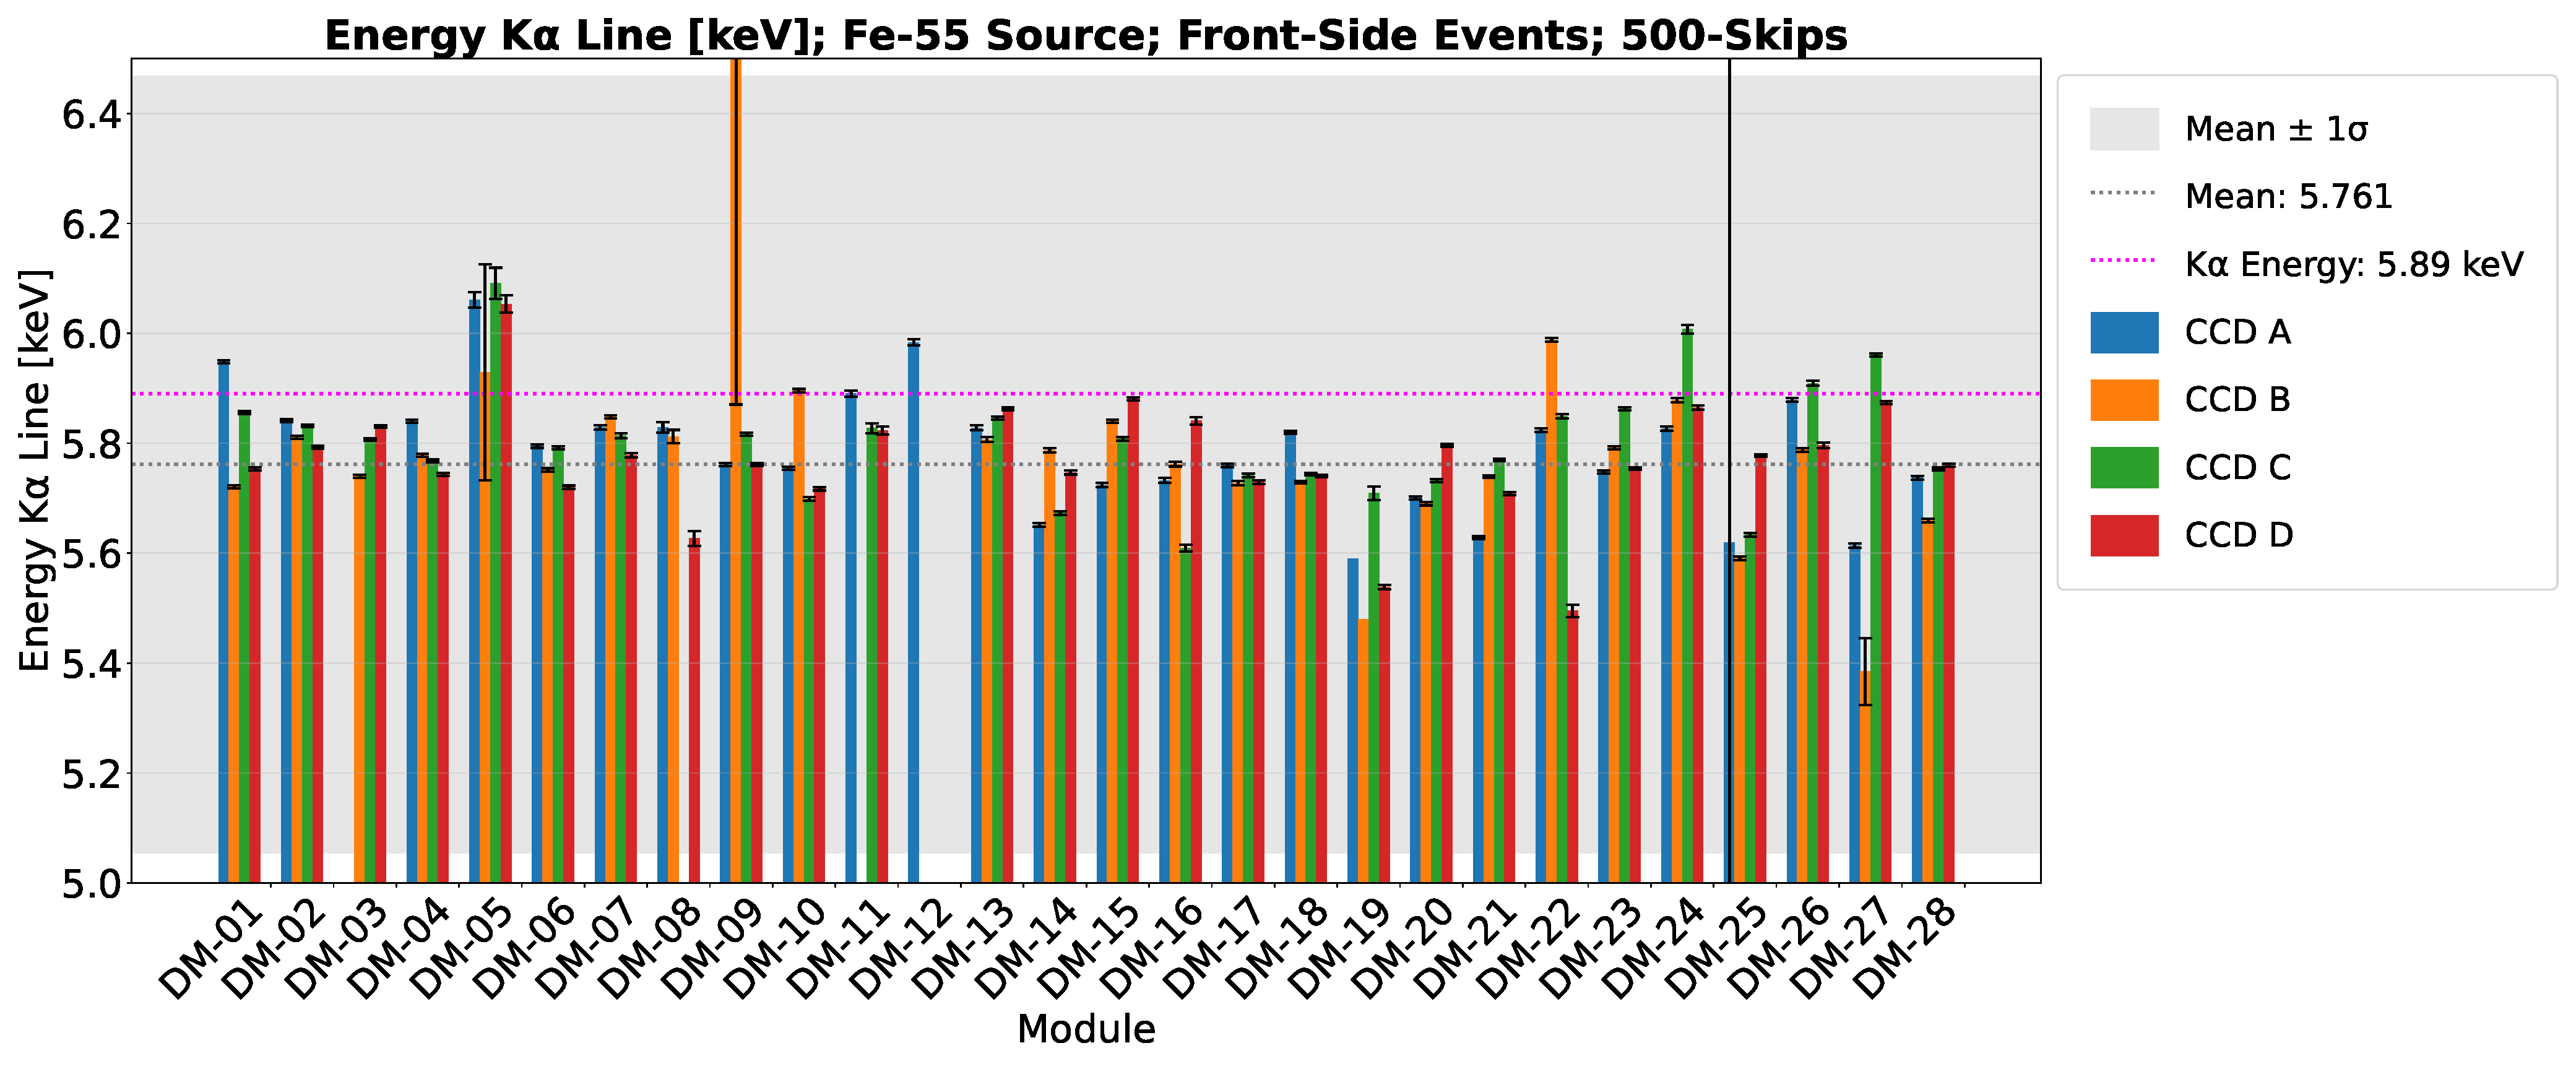
\includegraphics[width=0.95\linewidth]{figures/image5_low_peak1_all_modules.pdf}\\[0.3em]
    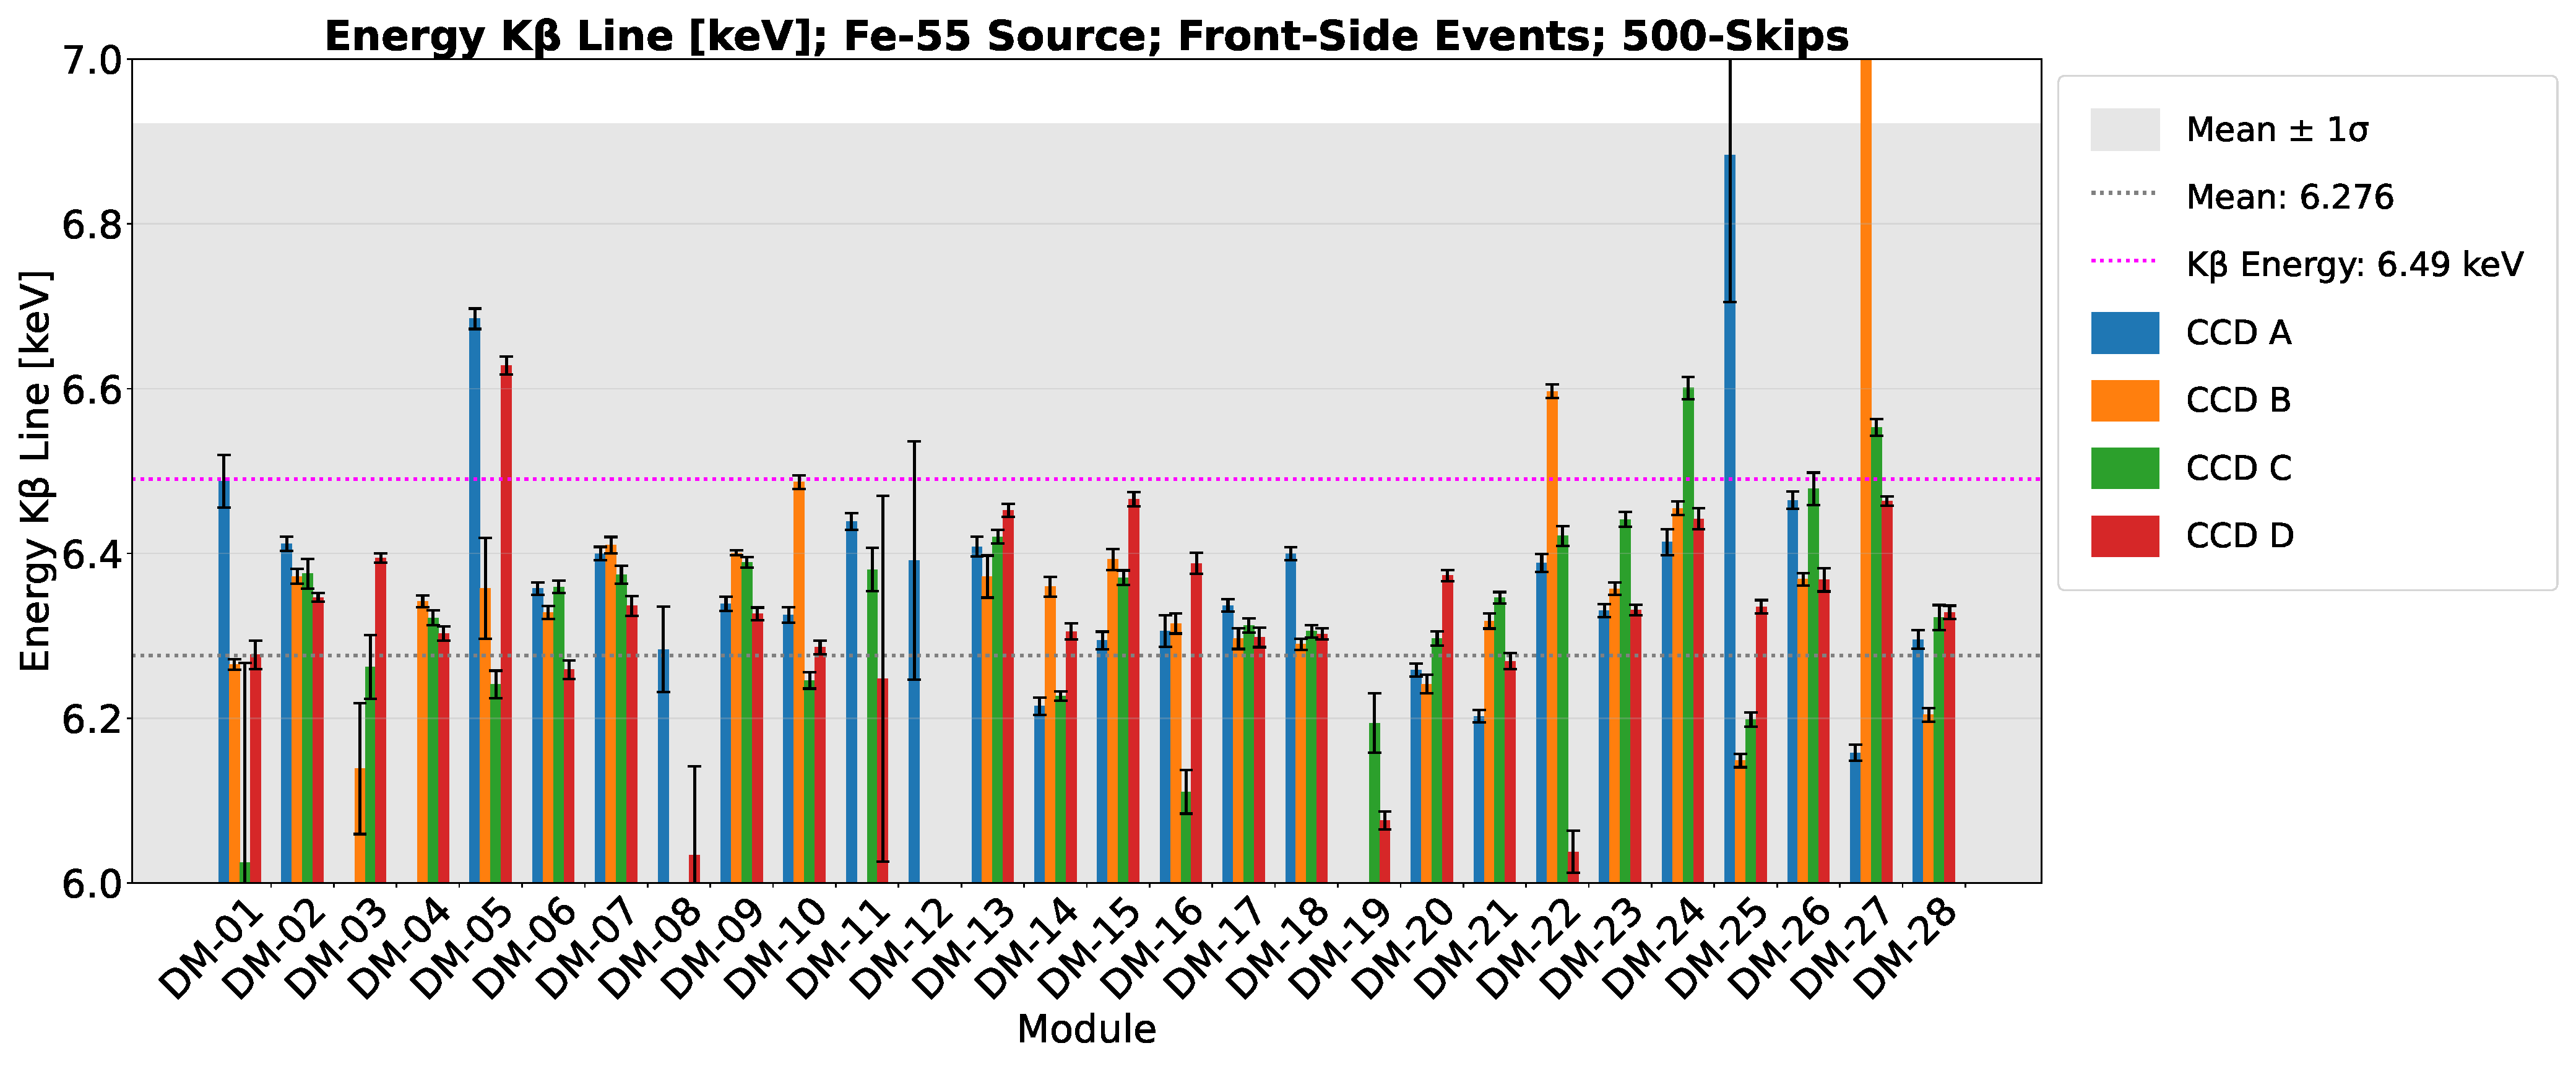
\includegraphics[width=0.95\linewidth]{figures/image5_low_peak2_all_modules.pdf}
    \caption[K$\alpha$/K$\beta$ line energies by module]{Fitted front-side Mn K$\alpha$ (top, nominal 5.89\,keV) and Mn K$\beta$ (bottom, nominal 6.49\,keV) line energies for each CCD extension across all production modules tested underground, from 500-skip Image\_5 data at 135\,K.}
    \label{fig:kev_lines_bymodule}
\end{figure}

Across the ensemble, both lines are reconstructed systematically below their nominal values: K$\alpha \approx 5.761$\,keV against an expected 5.90\,keV, and K$\beta \approx 6.276$\,keV against an expected 6.49\,keV, a shift of roughly 2--3\% observed consistently across CCDs and modules. A small number of modules deviate from this common trend in the opposite direction: DM-05 reconstructs both lines above the ensemble mean, and above the nominal energy itself in several extensions, while DM-19 reconstructs both lines below the ensemble mean, the most negative deviation in the dataset. A handful of individual extensions (e.g.\ DM-09, DM-25, and DM-27) show anomalously large statistical uncertainties in one or both lines, consistent with low-statistics fits rather than a distinct physical effect. The consistency and direction of the ensemble-wide shift -- essentially every module reconstructing low, rather than scattering symmetrically around the nominal value -- points to a systematic effect in the charge-to-energy conversion rather than module-to-module variation, motivating the pixel-charge nonlinearity study described next.

A dedicated high-statistics dataset near $500\,e^-$ was used to study the response of the skipper amplifier as a function of reconstructed charge. Figure~\ref{fig:nonlinearity} shows a clear nonlinear deviation between the reconstructed and expected pixel charge that grows with charge, and applying a nonlinear correction of this form is sufficient to account for the observed K$\alpha$/K$\beta$ energy-scale shift. The magnitude of the effect depends on both the amplifier and the operating parameters used, and is examined in more detail in a complementary, forthcoming study of amplifier nonlinearity. \todonote{We still need to cross-reference the forthcoming amplifier-nonlinearity study once it has a docdb number or draft.}

\begin{figure}[H]
    \centering
    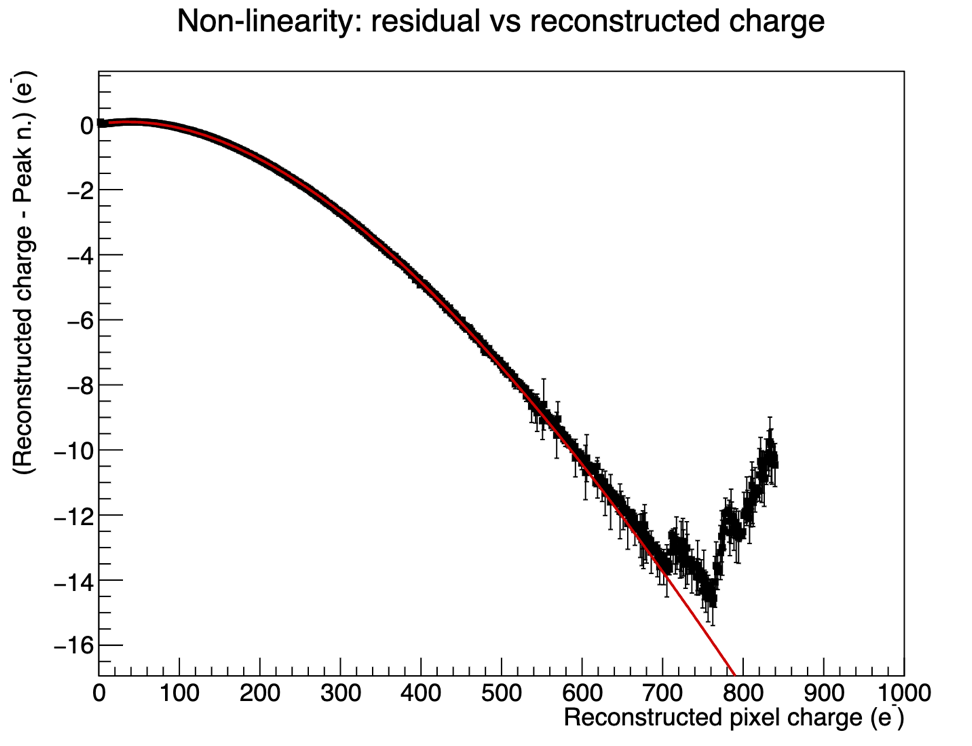
\includegraphics[width=0.75\linewidth]{figures/nonlinearity_residual.png}
    \caption[Pixel-charge nonlinearity]{Residual between the reconstructed pixel charge and the expected (peak-index) charge as a function of reconstructed charge, from a high-statistics dataset near $500\,e^-$. A clear nonlinear deviation develops above $\sim 400$--$500\,e^-$; the red curve is the nonlinear correction applied to account for the K$\alpha$/K$\beta$ energy-scale shift.}
    \label{fig:nonlinearity}
\end{figure}

Parameter scans were performed over the module biases and most rail voltages to identify the origin of the shift. The largest effect was found when lowering the reference voltage ($\mathrm{VR}$) from its nominal LBC science-run value of $-3$\,V to $-6$\,V, which reduces the observed nonlinear effect: Fig.~\ref{fig:vr_scan} compares the front/back energy spectra at the two settings, showing that $\mathrm{VR}=-6$\,V brings the front- and back-side K$\alpha$ peaks into much closer agreement than the nominal $\mathrm{VR}=-3$\,V setting. The revised parameters did not affect gain, single-electron resolution, or dark current significantly relative to the nominal LBC operating point.

\begin{figure}[H]
    \centering
    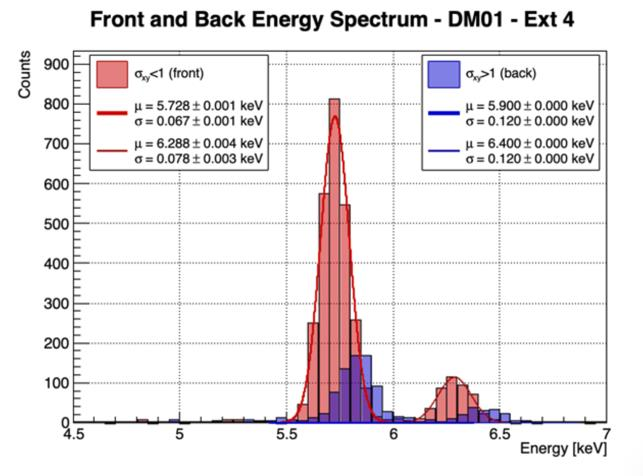
\includegraphics[width=0.48\linewidth]{figures/vr_scan_spectrum_VRm3V.png}
    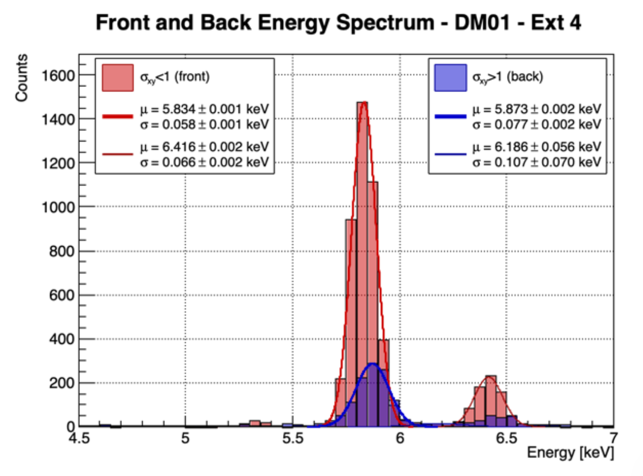
\includegraphics[width=0.48\linewidth]{figures/vr_scan_spectrum_VRm6V.png}
    \caption[Bias-voltage dependence of the energy-scale shift]{Front- ($\sigma_{xy}<1$, red) and back-side ($\sigma_{xy}>1$, blue) energy spectra for a representative extension (DM01, Ext.\ 4) at the nominal LBC operating point, $\mathrm{VR}=-3$\,V (left), and at $\mathrm{VR}=-6$\,V (right). Lowering VR shifts both lines closer to their nominal energies and brings the front- and back-side K$\alpha$ peaks into closer agreement ($\mu_{\mathrm{front}}=5.834$\,keV vs.\ $\mu_{\mathrm{back}}=5.873$\,keV at $\mathrm{VR}=-6$\,V, compared to $\mu_{\mathrm{front}}=5.728$\,keV vs.\ $\mu_{\mathrm{back}}=5.900$\,keV at $\mathrm{VR}=-3$\,V). \todonote{We still need to characterize the non-linearity at VR=-6\,V with higher statistics; we should flag this as a follow-up in the discussion.}}
    \label{fig:vr_scan}
\end{figure}

\subsection{Crosstalk}

Crosstalk occurs when a pixel in a source CCD with a genuine charge signal induces a small signal in the corresponding pixel of another CCD, called the destination CCD. This effect originates from electronic coupling between the readout channels. When accumulated over many events, it leads to a systematic linear correlation between the charges measured in corresponding pixels of the source (src) and destination (dst) CCDs. 

The crosstalk coefficient for a given (src, dst) pair quantifies the strength of this coupling. It is defined as the slope of the linear correlation between the simultaneous readouts of corresponding pixels in the two CCDs and is computed as follows.

First, seed pixels $[j,i]$ are selected in the source CCD such that their charge satisfies:

\begin{equation}
S_{\min} < q_{\mathrm{src}}[j,i] < S_{\max}
\end{equation}

For the results here shown, $S_{\min} = 400\,e^-$ and $S_{\max} = 10000\,e^-$.

Then, for each selected seed pixel, the charge ratio between the destination and source CCDs is computed as:
\begin{equation}
r_{j,i} =
\frac{q_{\mathrm{dst}}[j,i]}
     {q_{\mathrm{src}}[j,i]} .
\end{equation}

Finally, the crosstalk coefficient is defined as the median of the ratios over all selected seeds:

\begin{equation}
\alpha_{\,\mathrm{dst} \leftarrow \mathrm{src}}
=
\mathrm{Median}
\left(
\frac{q_{\mathrm{dst}}[j,i]}
     {q_{\mathrm{src}}[j,i]}
\right) .
\end{equation}

Repeating this procedure for all ordered CCD pairs produces the crosstalk matrix, which encodes the inter-CCD coupling coefficients.

Once the coefficients are determined, the raw charge in each CCD is corrected by subtracting the induced contributions from all other CCDs:

\begin{equation}
q_{\mathrm{dst}}^{\mathrm{corrected}} = q_{\mathrm{dst}}
-\sum_{\mathrm{src} \neq \mathrm{dst}}
(\alpha_{\,\mathrm{dst} \leftarrow \mathrm{src}} - \alpha_{\mathrm{null}})
\, q_{\mathrm{src}} .
\end{equation}

Here $\alpha_{\mathrm{null}}$ represents the null-hypothesis correction, which accounts for correlations arising from statistical fluctuations or selection effects. It is computed by randomizing the spatial positions of all seed pixels in the source image, breaking the correlation.


Figure~\ref{fig:CrosstalkDM16} shows the pairwise crosstalk characterization between the four CCD channels. Each panel corresponds to an ordered pair (src, dst), where the horizontal axis shows the source CCD pixel charge and the vertical axis shows the destination CCD pixel charge. Each blue point represents the charge for the selected seed pixels for both source and destination CCDs. The black line represents the computed linear correlation between the source and destination pixel charges; its slope corresponds to the crosstalk coefficient, and the red dashed line represents the linear correlation corrected under the null hypothesis.


\begin{figure}[H]
    \centering
    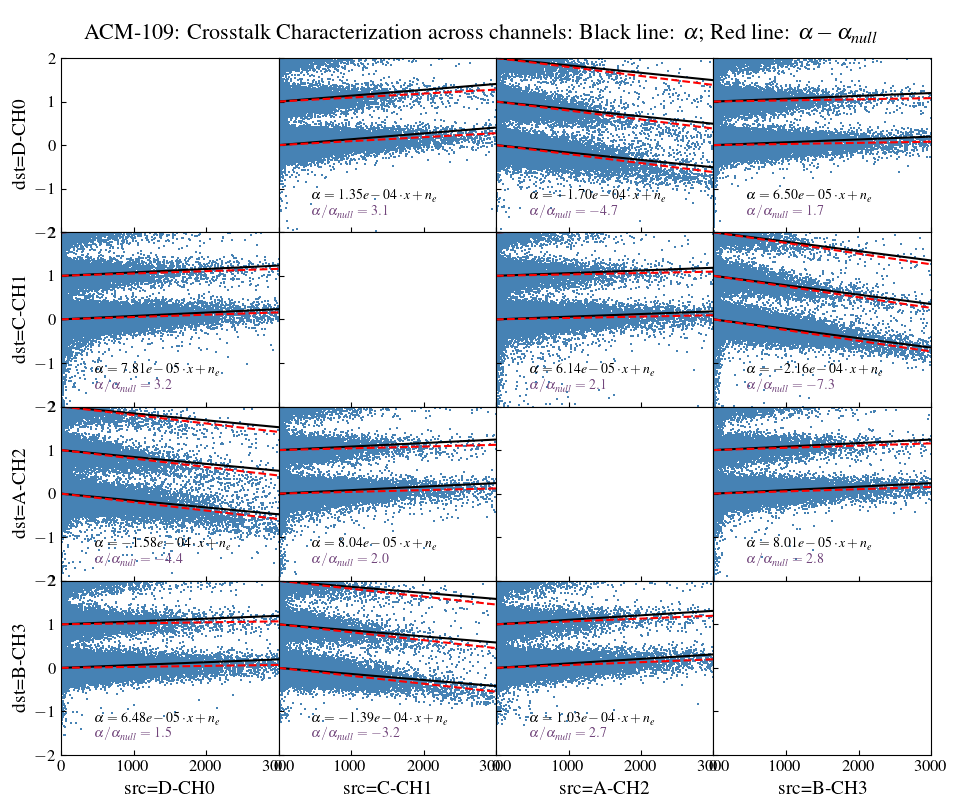
\includegraphics[width=0.7\linewidth]{figures/DM16_xtalk.png}
    \caption{Crosstalk characterization between CCD channels for module DM16 which corresponds with ACM 109.}
    \label{fig:CrosstalkDM16}
\end{figure}

The following modules were processed with the number of images used per module indicated in parentheses: DM3(2), DM14(3), DM17(2), DM20(3), DM23(3), DM28(2); DM2(2), DM9(2), DM13(3), DM16(2), DM19(3), DM22(3), DM27(3); DM1(2), DM7(2), DM15(2), DM18(3), DM21(3).


Figure~\ref{fig:CrosstalkAll} summarizes the null-hypothesis–corrected crosstalk coefficients obtained for the studied modules. Each panel corresponds to an ordered (src, dst) pair, with the vertical axis indicating the source CCD and the horizontal axis the destination CCD. Within each panel, the bars represent the null-hypothesis–corrected crosstalk coefficient obtained for each module. The horizontal dashed line denotes the overall mean crosstalk coefficient across all modules for the given (src, dst) pair, while the shaded gray band indicates the $\pm 1\sigma$ dispersion. Red bars correspond to positive crosstalk coefficients, and blue bars to negative ones.

\begin{figure}[H]
    \centering
    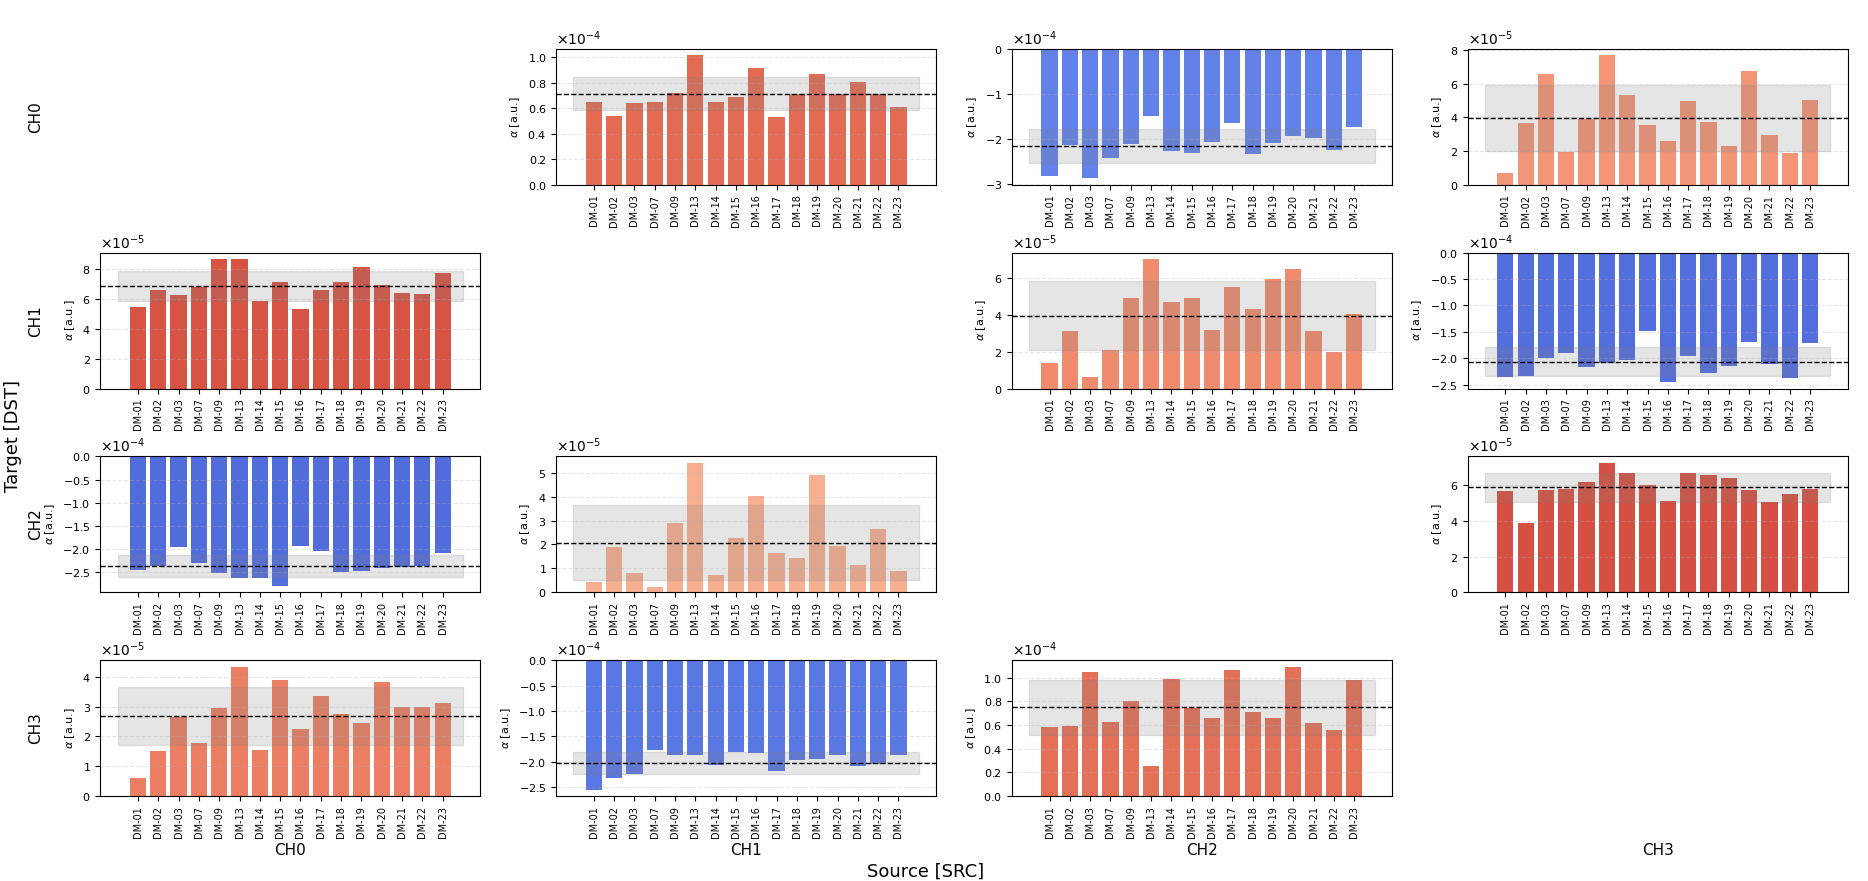
\includegraphics[width=0.9\linewidth]{figures/xtalk_allmodules.png}
    \caption{Null-hypothesis–corrected crosstalk coefficients obtained for all studied modules.}
    \label{fig:CrosstalkAll}
\end{figure}

This study concluded that a single crosstalk correction matrix can be consistently applied across all ACMs and modules. However, not all modules were analyzed, as the current methodology is not suitable for determining crosstalk in modules with high dark current.

\FloatBarrier

\subsection{Recommendation for outermost array positions}
\label{sec:outermost_modules}

Four modules must be placed in the outermost positions of the final DAMIC-M array. The per-module metrics compiled in Table~\ref{tab:summary_metrics} were used to select these four.

DM11 is a first, unambiguous choice: as noted in Sec.~\ref{sec:summary}, Extension 2 of DM11 was found to be non-functional at LSM, in contrast to its performance during on-surface testing, so DM11 already operates as a three-CCD module rather than four.

The remaining three positions were selected using dark current as the primary discriminating metric, consistent with the approach used elsewhere in this report, and cross-checked against single-electron resolution (SER) and CTI. Ranked by dark current, and excluding DM11 as well as DM08 and DM12 (already excluded from the final array), the three highest-dark-current modules are DM10, DM26, and DM24, summarized in Table~\ref{tab:outermost_candidates} alongside DM11 and the ensemble mean for reference.

\begin{table}[H]
\centering
\caption{Module-level metrics (from Table~\ref{tab:summary_metrics}) for the four modules recommended for the outermost array positions.}
\label{tab:outermost_candidates}
\renewcommand{\arraystretch}{1.2}
\begin{tabular}{@{}lcccccc@{}}
\toprule
Module
& \makecell{Operational \\ CCDs}
& \makecell{Gain \\ (e$^{-}$/ADU)}
& \makecell{SER $\sigma$ \\ (e$^{-}$)}
& \makecell{Dark current \\ (e$^{-}$/pix/day)}
& \makecell{CTI \\ Parallel fraction}
& \makecell{CTI \\ Serial fraction} \\
\midrule
DM11 & 3 & 1.3893 & 0.1331 & 0.1297 & 0.00165 & 0.00623 \\
DM10 & 4 & 1.2870 & 0.1438 & 3.2194 & 0.00683 & 0.00078 \\
DM26 & 4 & 1.2760 & 0.1409 & 1.5180 & 0.01036 & 0.00127 \\
DM24 & 4 & 1.3160 & 0.1374 & 0.8753 & 0.00503 & 0.00110 \\
\midrule
Ensemble mean & -- & -- & -- & 0.388 & -- & -- \\
\bottomrule
\end{tabular}
\end{table}

DM10 shows the highest dark current of any operational module in the array, consistently across two independent installations (Sec.~\ref{sec:summary}), making it an unambiguous choice. DM26 and DM24 rank second and third; the Executive Summary notes that dark current initially observed in DM24, DM25, and DM26 was attributed to an installation issue and reported as restored to average levels after a second installation, though the values in Table~\ref{tab:summary_metrics} remain above the ensemble mean for all three. Neither SER nor CTI flags DM10, DM26, or DM24 as anomalous on those metrics individually, so dark current remains the primary driver of this ranking.

The four modules recommended for the outermost array positions are therefore DM10, DM11, DM24, and DM26.

\FloatBarrier

% =====================================================
%                     Conclusions
% =====================================================
\newpage
\section{Conclusions}
\label{sec:conclusions}

This report has presented the underground characterization of the 28 DM production modules tested at LSM between May and October 2025, evaluated against the sensor-level performance requirements of the DAMIC-M experiment. Of the modules tested, 103 CCDs are operational in the final array configuration, spread across 26 modules with four operational CCDs each except DM11, which has three, for an effective target mass of approximately 347\,g (Sec.~\ref{sec:summary}).

Across the ensemble, single-electron resolution, amplifier gain, and dark current at 135\,K are consistent with expectations for most extensions, with column and serial-register defect rates remaining low overall (Secs.~\ref{sec:hightemp}, \ref{sec:lowtemp}). Vertical (parallel-direction) charge transfer inefficiency is consistently observed across the module set under nominal LBC operating parameters, and DM-12 in particular shows a genuine directional asymmetry in its back-side cluster morphology that merits further investigation (Sec.~\ref{sec:CTI}). The keV-scale energy-scale shift observed in the $^{55}$Fe calibration lines is well explained by pixel-charge nonlinearity in the skipper amplifier response, and is partially mitigated by lowering the reference voltage to $\mathrm{VR}=-6$\, V (Sec.~\ref{sec:kev_calibration}). A single crosstalk correction matrix was consistently applicable across all ACMs and modules tested.

DM-08 and DM-12 are excluded from the final detector array due to a large column defect and associated amplifier glow (DM-08) and non-operational extensions (DM-12). Based on dark current as the primary discriminating metric, cross-checked against single-electron resolution and CTI, DM10, DM11, DM24, and DM26 are recommended for the outermost positions of the final array (Sec.~\ref{sec:outermost_modules}).

Two items remain open following this campaign. The apparent failure of Extension 2 in DM11, which operated normally during on-surface testing at UW but was found non-functional at LSM, warrants investigation of its wire bonding before final array integration. In addition, the residual pixel-charge nonlinearity at $\mathrm{VR}=-6$\,V still needs higher-statistics characterization to confirm that the revised bias point fully addresses the energy-scale shift.

% =====================================================
%                       Appendix
% =====================================================
\newpage
\appendix
\section{Appendix}
\label{sec:appendix}

\subsection{Additional plots}

\paragraph{Detector status.} Of the 28 modules tested underground, 103 CCDs are operational in the final detector configuration, spread across 26 production modules with four CCDs each, except DM11, which has three (Ext.\ 2 was found non-functional despite working during the on-surface campaign at UW). DM08 and DM12 are excluded from the final array due to non-operational extensions and large defects; all plots and summary statistics elsewhere in this report that quote ensemble averages exclude these two modules unless noted otherwise. The effective target mass of the final array is $\approx 347$\,g. DM10, DM24, DM25, and DM26 exhibit consistently higher dark current than the rest of the ensemble (Sec.~\ref{sec:lowtemp}), and vertical (parallel-direction) CTI is observed across modules under the nominal LBC operating parameters (Sec.~\ref{sec:CTI}); lowering $\mathrm{VR}$ to $-6$\,V reduces the $^{55}$Fe energy-scale shift, though the resulting non-linearity still needs to be characterized with higher statistics (Sec.~\ref{sec:kev_calibration}).

Table~\ref{tab:summary_metrics} gives the full per-module breakdown of these metrics (operational CCDs, gain, SER, dark current, and CTI fractions).

% Example: include a per-CCD grid of something
% \figgridfour
%   {figures/lowT/CCD1/noise_map.pdf}
%   {figures/lowT/CCD2/noise_map.pdf}
%   {figures/lowT/CCD3/noise_map.pdf}
%   {figures/lowT/CCD4/noise_map.pdf}
%   {Noise maps (Low-T) for each CCD in module \ModuleID.}
%   {fig:appendix_noise_maps}

% =====================================================
%                    Bibliography
% =====================================================
% Added 2026-07-08 (Phase 3 of completeness audit) --- the document had
% \cite{} commands throughout but no \bibliography call at all, so nothing
% could ever have rendered. See references.bib in this folder.
\bibliographystyle{unsrt}
\bibliography{references}

\end{document}

